\documentclass[a4paper,12pt]{article} % тип документа

%  Русский язык
\usepackage{mathtext}               % русский язык в формулах
\usepackage[T2A]{fontenc}			% кодировка
\usepackage[utf8]{inputenc}			% кодировка исходного текста
\usepackage[english,russian]{babel}	% локализация и переносы

\usepackage{graphicx}               % импорт изображений
\usepackage{wrapfig}                % обтекаемые изображения
\graphicspath{{pictures/}}          % обращение к подкаталогу с изображениями
\usepackage{amsfonts}               % буквы с двойными штрихами
\usepackage{indentfirst}            % indent first
\usepackage{amsmath}                % можно выводить фигурные скобочки -- делать системы уравнений
\usepackage[table,xcdraw]{xcolor}   % таблицы
\usepackage{amsmath,amsfonts,amssymb,amsthm,mathtools} % Математика
\usepackage{wasysym}                % ???
\usepackage{upgreek}                % ???  

\usepackage{gensymb} % degree symbol
\usepackage{mathrsfs}

\usepackage{tikz}
\usetikzlibrary{graphs,graphs.standard}

\usepackage{cancel} % перечеркивания

%% Интервалы
\linespread{1}
\usepackage{multirow}

%% Перенос знаков в формулах (по Львовскому)
\newcommand*{\hm}[1]{#1\nobreak\discretionary{}
	{\hbox{$\mathsurround=0pt #1$}}{}}

%% Русские списки
\usepackage{enumitem}
\makeatletter
\AddEnumerateCounter{\asbuk}{\russian@alph}
\makeatother

% Дополнительная работа с математикой
\usepackage{amsmath,amsfonts,amssymb,amsthm,mathtools} % AMS
\usepackage{icomma} % "Умная" запятая: $0,2$ --- число, $0, 2$ --- перечисление

\usepackage{dsfont}
\usepackage{cancel} % перечеркивания

%%% Свои команды
\DeclareMathOperator{\sgn}{\mathop{sgn}}

%%% Программирование
\usepackage{etoolbox} % логические операторы

%%% Страница
\usepackage{extsizes} % Возможность сделать 14-й шрифт
\usepackage{geometry} % Простой способ задавать поля
	\geometry{top=20mm}
	\geometry{bottom=20mm}
	\geometry{left=20mm}
	\geometry{right=20mm}
	
\usepackage{mathrsfs}

\newcommand{\eqdef}{\stackrel{\mathrm{def}}{=}}
\newcommand{\ryad}{\sum\limits^{\infty}_{k = 0}}

\newcommand{\R}{\mathbb{R}}
\newcommand{\N}{\mathbb{N}}
\newcommand{\series}{\sum\limits_{k=1}^{\infty}}
\newcommand{\useries}{\sum\limits_{k=1}^{\infty} u_k}
\newcommand{\useriesl}{\sum\limits_{k=1}^{\infty} u_k < \infty}
\newcommand{\useriese}{\sum\limits_{k=1}^{\infty} u_k = \infty}
\newcommand{\auseries}{\sum\limits_{k=1}^{\infty} |u_k|}
\newcommand{\auseriesl}{\sum\limits_{k=1}^{\infty} |u_k| < \infty}
\newcommand{\auseriese}{\sum\limits_{k=1}^{\infty} |u_k| = \infty}
\newcommand{\sn}{\sum\limits_{k=1}^{n} u_k}

\renewcommand {\ge}{\geqslant}
\renewcommand {\le}{\leqslant}
\renewcommand {\geq}{\geqslant}
\renewcommand {\leq}{\leqslant}
\renewcommand {\epsilon}{\varepsilon}

\usepackage{titlesec}
\titlelabel{\thetitle.\quad}
%%% Для точек после названий секций

\usepackage{hyperref}
%%% Настройка ссылок
\hypersetup
{
	colorlinks = true,
	linkcolor  = black,
	filecolor  = magenta,
	urlcolor   = blue
}
%%% Конец настройки ссылок


\begin{document}

%=======================================================================================

\begin{titlepage}
\begin{center}
\
\vfill

{\LARGE \textsc{\textbf{Глоток свежевыжатого воздуха\\}}}

\vspace{2em}

Гончаренко Валентина, 1 курс ФРКТ, группа Б01-009

\vfill

Июнь 2021
\end{center}
\end{titlepage}

%=======================================================================================

\newpage
\tableofcontents{} %содержание
\newpage

%1
%=======================================================================================

\section{Введение}

<<Окружающий нас атмосферный воздух вследствие непрерывного испарения воды с поверхности водоёмов и растительных покровов всегда содержит в себе водяные пары. Содержание водяного пара в атмосфере характеризует такое понятие, как <<влажность>>. Она имеет большое значение для многих процессов, происходящих в атмосфере. Влажность воздуха характеризует погоду и климат, влияет на теплообмен организма с окружающей средой, на жизнь животных и растений...>> --- такими строчками Александр Васильевич Перышкин, автор учебника, ввёл нас <<в курс дела>> в 8 классе. Мой учитель физики тогда отметил, что в нашей подмосковной местности высокая влажность воздуха: <<Любили русские цари и императоры столицы на болотах строить...>>. 

Когда я училась в старшей школе, уже другой преподаватель физики отметил, что он избегает отдыха в Сочи из-за заоблачных для него показателей влажности, да и про Московскую область его отзывы были похожими. 

Действительно, влажность не только определяет комфортность атмосферы помещений, но и является важным экологическим показателем. Влажность оказывает серьезное влияние на наше здоровье, общее эмоциональное состояние. Слишком высокая влажность может привести к увеличению биологических загрязнителей, таких как плесень, бактерии, вирусы и грибки, которые могут вызвать аллергию и различные респираторные заболевания. При сильно влажном воздухе возможны обострения и приступы. При температуре окружающей среды +25°C и выше и одновременно влажном воздухе нарушается отдача тепла с поверхности кожи, и организм может перегреться.

Во избежание всех вышеперечисленных невзгод существуют осушители воздуха - приборы, основанные на различных физических принципах, которые помогают снизить влажность воздуха в помещении, автоматически поддерживая комфортные условия окружающей среды. В процессе поиска темы вопроса по выбору мой семинарист, Андрей Александрович Желтоухов, натолкнул меня на мысль о возможности ликвидации влаги из воздуха с помощью модуля Пельтье. В данной работе был изучен принцип действия осушителя на элементе Пельтье, была собрана модель такого типа осушителя и был проведен эксперимент, целью которого стала эмпирическая проверка некоторых теоретических соотношений.


\newpage

%2
%=======================================================================================

\section{Устройство и принцип работы}
Осушители, основанные на технологии Пельтье --- это приборы, в которых присутствует термоэлектрический преобразователь. Принцип его действия базируется на эффекте Пельтье --- возникновении разности температур при протекании электрического тока.

\begin{wrapfigure}[12]{r}{0.28\linewidth}
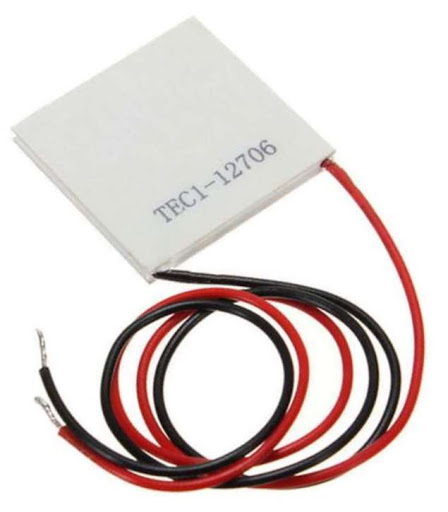
\includegraphics[width=4cm]{pictures/pict/unnamed.jpg}
\label{fig:image}
\caption{Внешний вид}
\end{wrapfigure}
В основе работы элементов Пельтье (рис. 1) лежит контакт двух токопроводящих материалов с разными уровнями энергии электронов в зоне проводимости. При протекании тока через контакт таких материалов электрон должен приобрести энергию, чтобы перейти в более высокоэнергетическую зону проводимости другого полупроводника. При поглощении этой энергии происходит охлаждение места контакта полупроводников. При протекании тока в обратном направлении происходит нагревание места контакта полупроводников, дополнительно к обычному тепловому эффекту.
При контакте металлов эффект Пельтье очень мал на фоне омического нагрева и явлений теплопроводности. Поэтому при практическом применении используются контакты двух полупроводников.

\begin{wrapfigure}[15]{l}{0.5\linewidth}
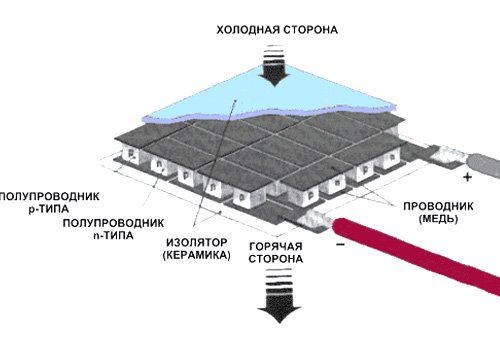
\includegraphics[width=8cm]{pictures/Cooler-Peltier-03.jpg}
\label{fig:image}
\caption{Внутреннее устройство}
\end{wrapfigure}

Единичный элемент термоэлектрического модуля – это термопара, представляющая собой объединение p- и n-проводника. Если последовательно соединить несколько подобных элементов, то поглощение теплоты будет происходить на n-p-контакте, а выделение на p-n-контакте. Элемент Пельтье состоит из одной или более пар полупроводниковых параллелепипедов (рис. 2). Пары параллелепипедов соединяются, образуя последовательное соединение многих пар полупроводников с разным типом проводимости так, чтобы вверху были одни последовательности соединений, а снизу противоположные. 

\begin{wrapfigure}[15]{r}{0.35\linewidth}
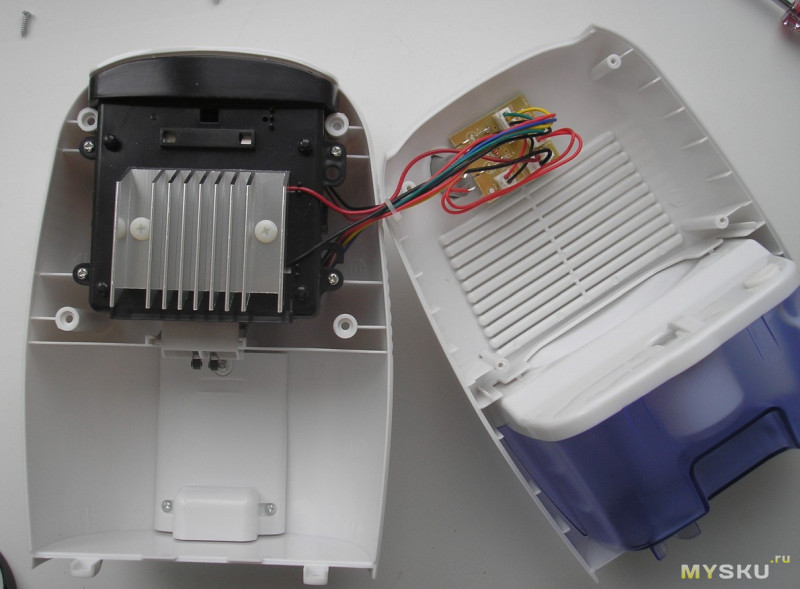
\includegraphics[width=6cm]{pictures/dry.jpg}
\label{fig:image}
\caption{XRow-600A осушитель на элементе Пельтье}
\end{wrapfigure}
Электрический ток протекает последовательно через все параллелепипеды. В зависимости от направления тока верхние контакты охлаждаются, а нижние нагреваются, или наоборот. Таким образом, электрический ток переносит тепло с одной стороны элемента Пельтье на противоположную и создаёт разность температур. Если охлаждать нагревающуюся сторону элемента Пельтье, то температура холодной становится ещё ниже.

Большинство осушителей выпускается компрессионного типа. Принцип действия основан на конденсации водяного пара, содержащегося в воздухе, на поверхностях испарителя с низкой температурой. По сути осушитель воздуха представляет собой кондиционер, в котором отвод тепла происходит в то же помещение. На рис. 3 фото разобранного осушителя заводского производства.


\newpage

%3
%=======================================================================================

\section{Схема и собранная модель}

Собранная модель представляет из себя конструкцию, показанную на рис. 4. Электрическая схема и фото процесса представлены на рис. 5. Дополнительные фото вынесены в приложения.

Источником электроэнергии служит блок питания компьютера на 12В. Система охлаждения горячей стороны элемента Пельтье состоит из вентилятора от того же компьютера. Радиаторы являются предупредителями перегрева и переохлаждения элемента. Для улучшения процесса теплопередачи использовалась термопаста.

\begin{figure}[h!]
	\centering
	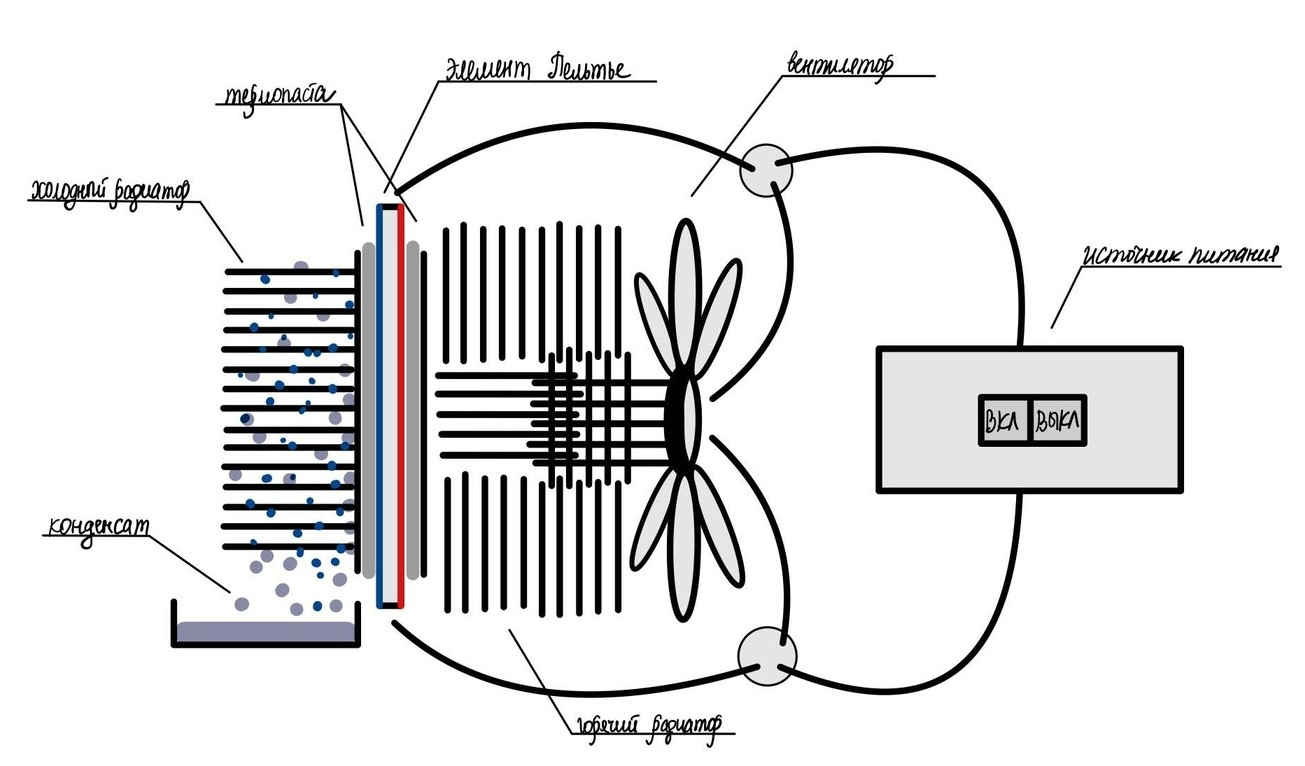
\includegraphics[scale=0.4]{pic.jpg}
	\caption{Схема сборки}
\end{figure}

\begin{figure}[ht]\center
\begin{tabular}{cc}
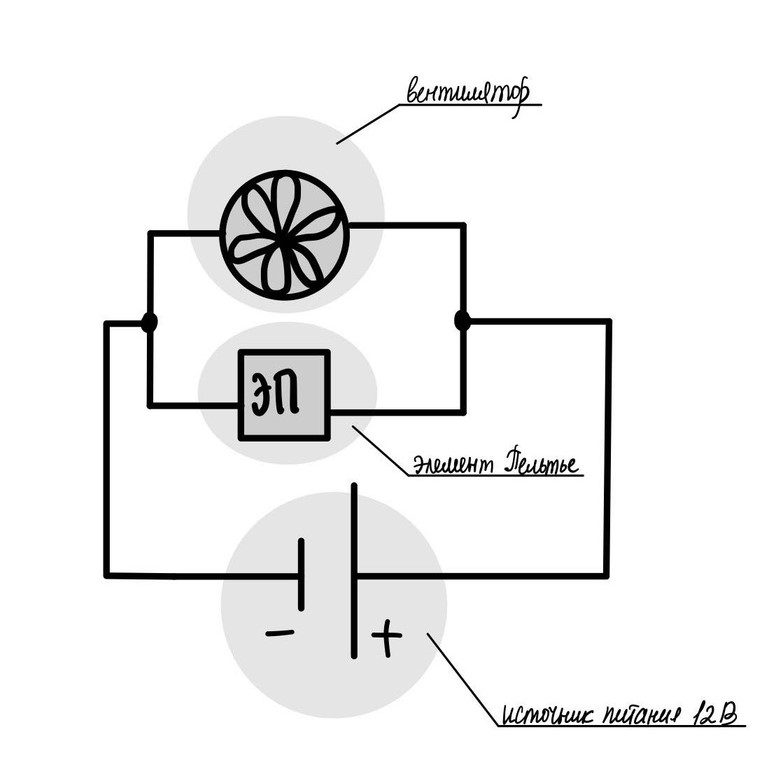
\includegraphics[width=75mm]{ch.jpg}
&
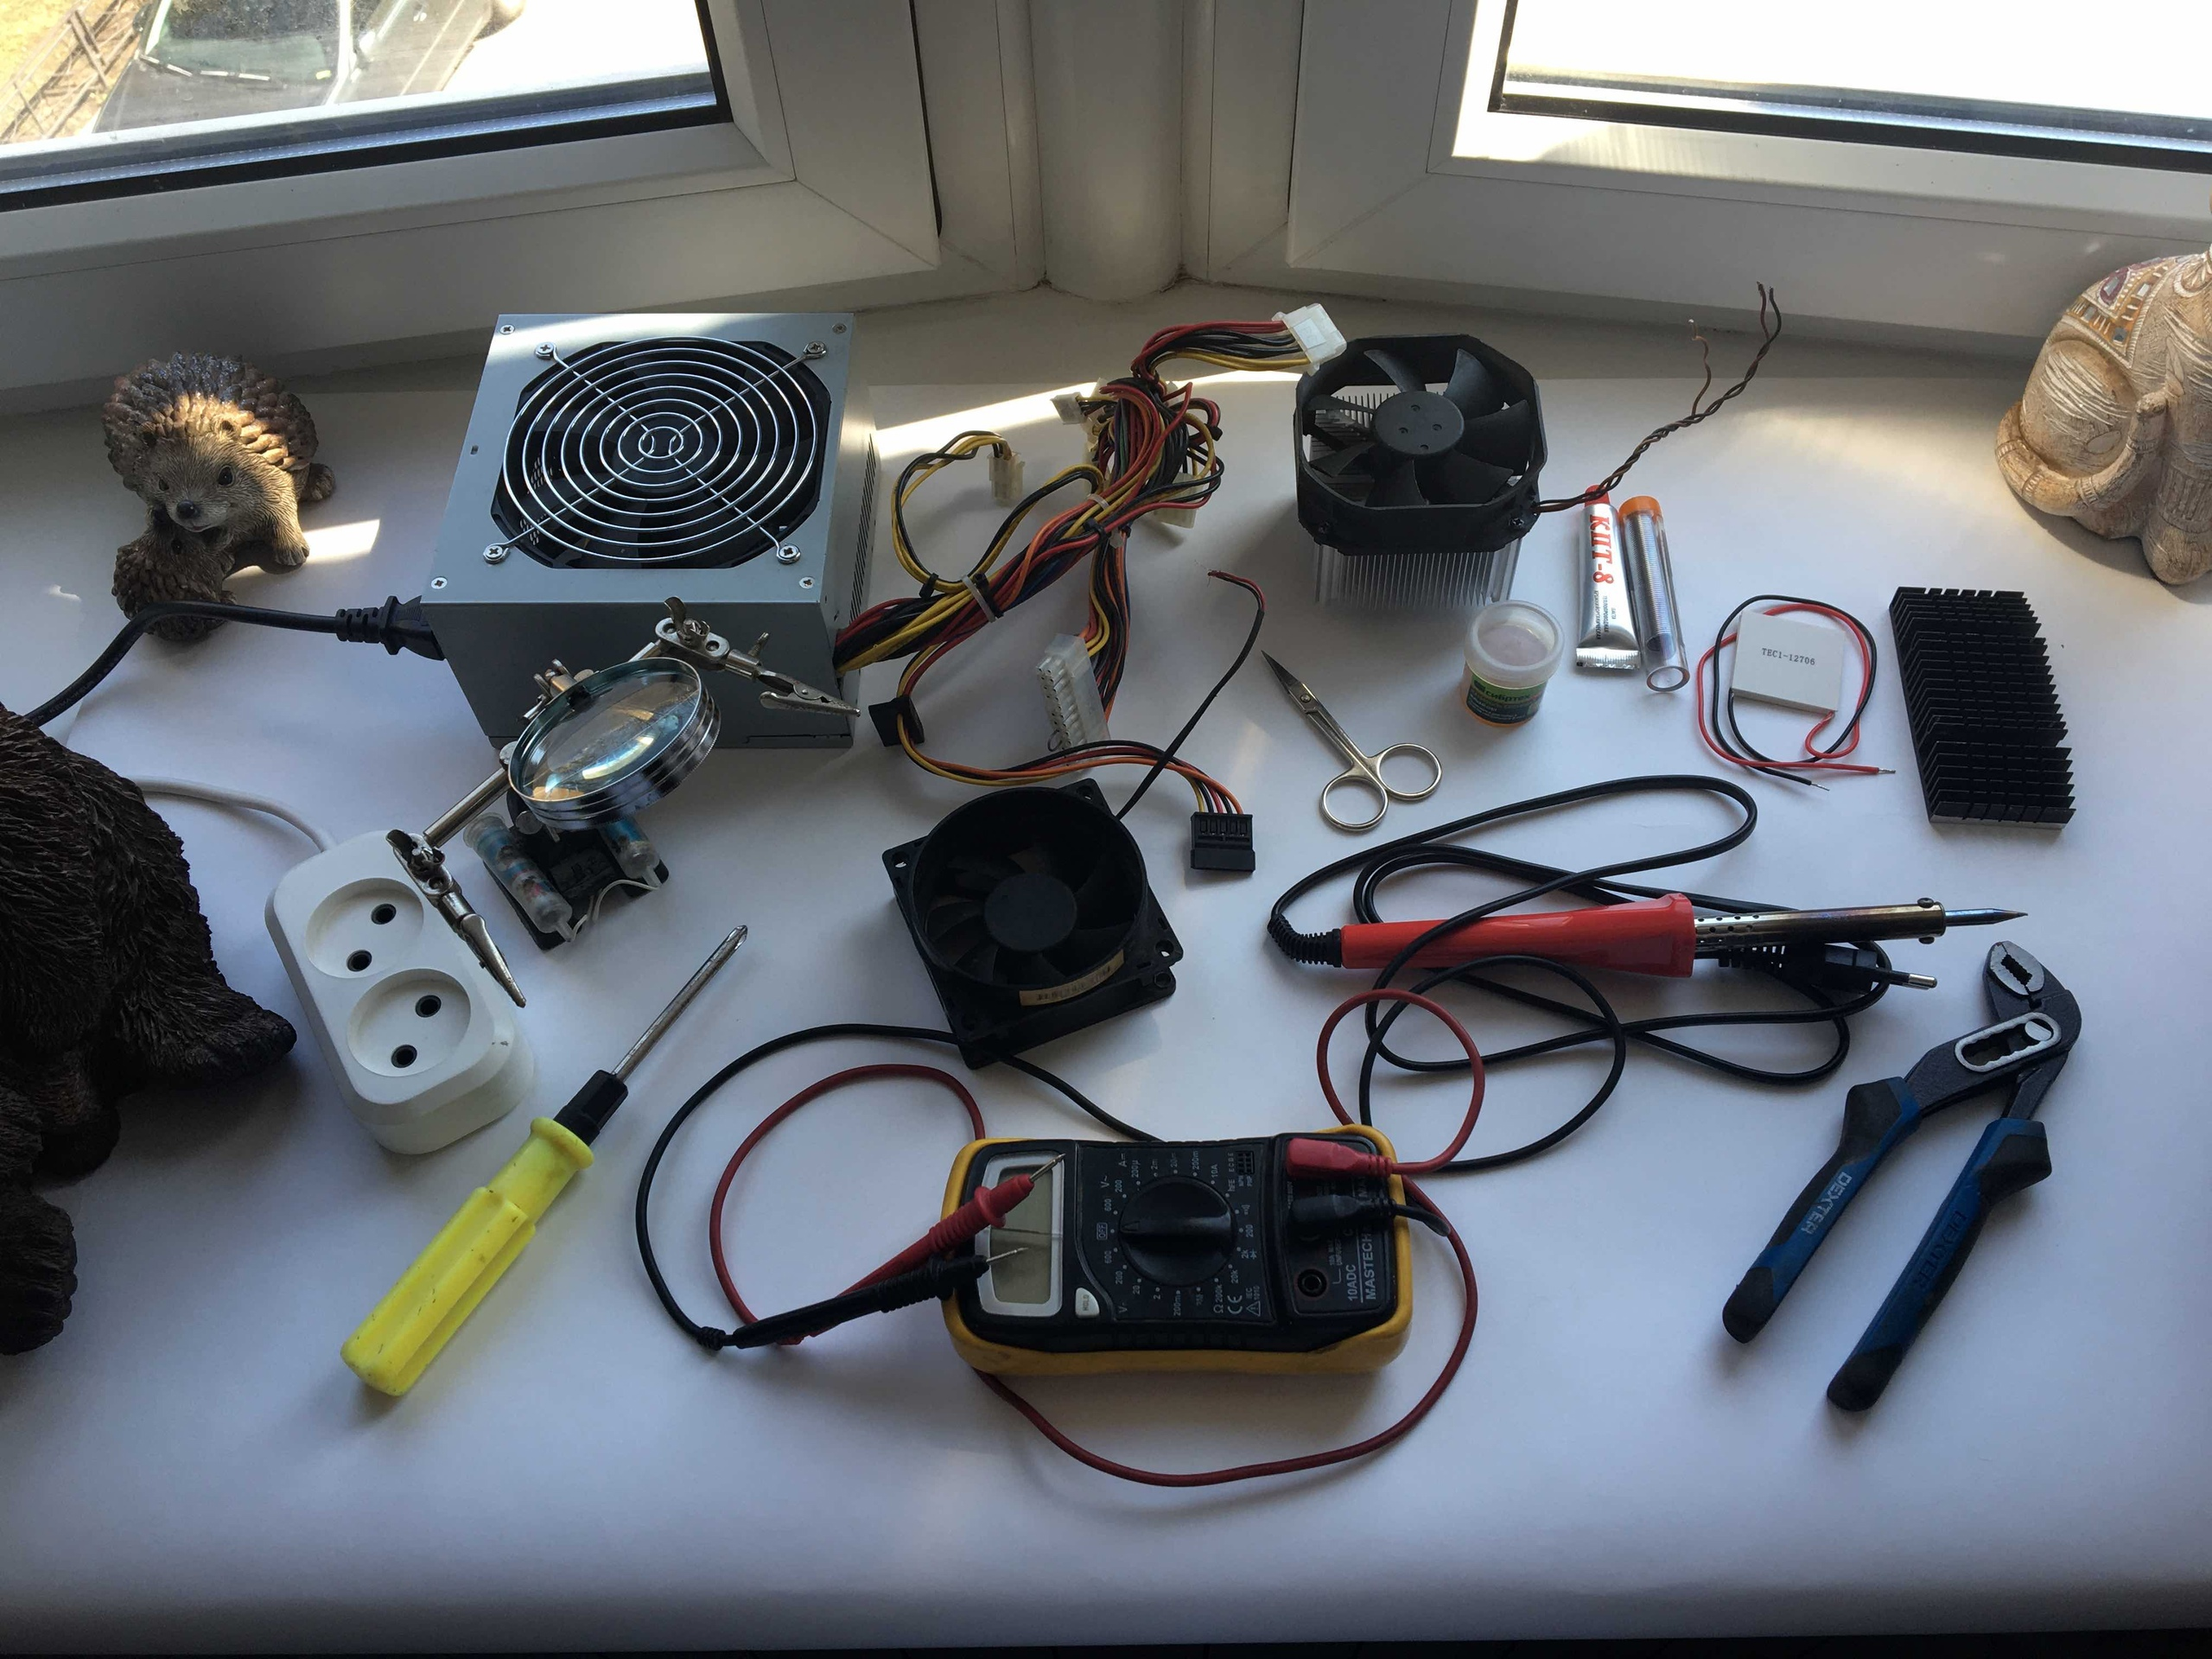
\includegraphics[width=90mm]{xex.jpg}
\end{tabular}
\caption{Электрическая схема и процесс сборки}
\end{figure}

\newpage

%4
%=======================================================================================

\section{Преимущества и недостатки}

К достоинствам осушителя на элементе Пельтье можно отнести:

\hspace{5mm}
1. Отсутствие механически движущихся частей, газов, жидкостей.

\hspace{5mm}
2. Бесшумную работу (если не учитывать звук охлаждающей системы).

\hspace{5mm}
3. Небольшие размеры.

\vspace{5mm}

Недостатки заключаются в следующем:

\hspace{5mm}
1. Весьма низкий коэффициент полезного действия.

\hspace{5mm}
2. Необходимость в источнике питания.

\hspace{5mm}
3. Высокая стоимость мощных модулей Пельтье.

\hspace{5mm}
4. Неизбежность дополнительной терморегуляции для контроля работоспособности устройства и продолжения срока его службы.


\newpage

%5
%=======================================================================================

\section{Эксперимент}

В основу эксперимента была положена следующая теоретическая модель: 

\vspace{2mm}
{\it Если измерить концентрации водяных паров в помещении в начале и в конце эксперимента, то можно вычислить гипотетический объём конденсата и сравнить его с реальной величиной.}

\vspace{2mm}
В качестве помещения была взята коробка из-под газонокосилки (пропорционально масштабам и мощности осушителя, далее --- помещение $\equiv$ коробка). Температура на холодном радиаторе измерялась термопарой, температура и концентрация водных паров в помещении отслеживались с помощью психрометрического гигрометра ВИТ-2 (жидкость в стеклянном питателе - дистиллированная вода).

Обозначим  $T_0$ температуру в помещении, $n_0, n_1$ --- концентрации водяных паров в начале и в конце эксперимента соответственно. В течение опыта температура помещения поддерживается постоянной. Запишем выражение для массы конденсата: $$\Delta m = m_0 - m_1 = (n_0 - n_1 )Vm_{mol},$$ где $V$ и $m_{mol}$ - объем помещения и масса одной молекулы соответственно. Тогда $$\Delta m = (\rho_0 - \rho_1 )V,$$ где $\rho_0$ и ${\rho_1$ - плотности водяных паров в начале и в конце эксперимента (г/м^3). 

$$\Delta m = \rho (T_0)(\varphi_0 - \varphi_1)V,$$ где $\varphi_0$ и $\varphi_1$ - относительные влажности в начале и в конце опыта. 

\vspace{2mm}
Температура $T_0$ в процессе эксперимента: \approx 23,5$^\circ$С

Объем помещения: ($l$) 0,79 м $\times$ ($w$) 0,51 м $\times$ ($h$) 0,62 м

Плотность $\rho (T_0)$: \approx 20,8 $ г/м^3$

$\varphi_0$ (психрометрическая таблица): 91\%

$\varphi_1$ (психрометрическая таблица): \approx 65,5\%

Теоретическое значение $\Delta m$ $\approx 20,8\cdot(0,91 - 0,655)\cdot0,79\cdot0,51\cdot0,62 \approx 1,32$ г, тогда объём сконденсировавшейся жидкости равен $\Delta v$ $\approx 1,32$ мл.
\begin{figure}[h!]
\center
\begin{tabular}{cc}
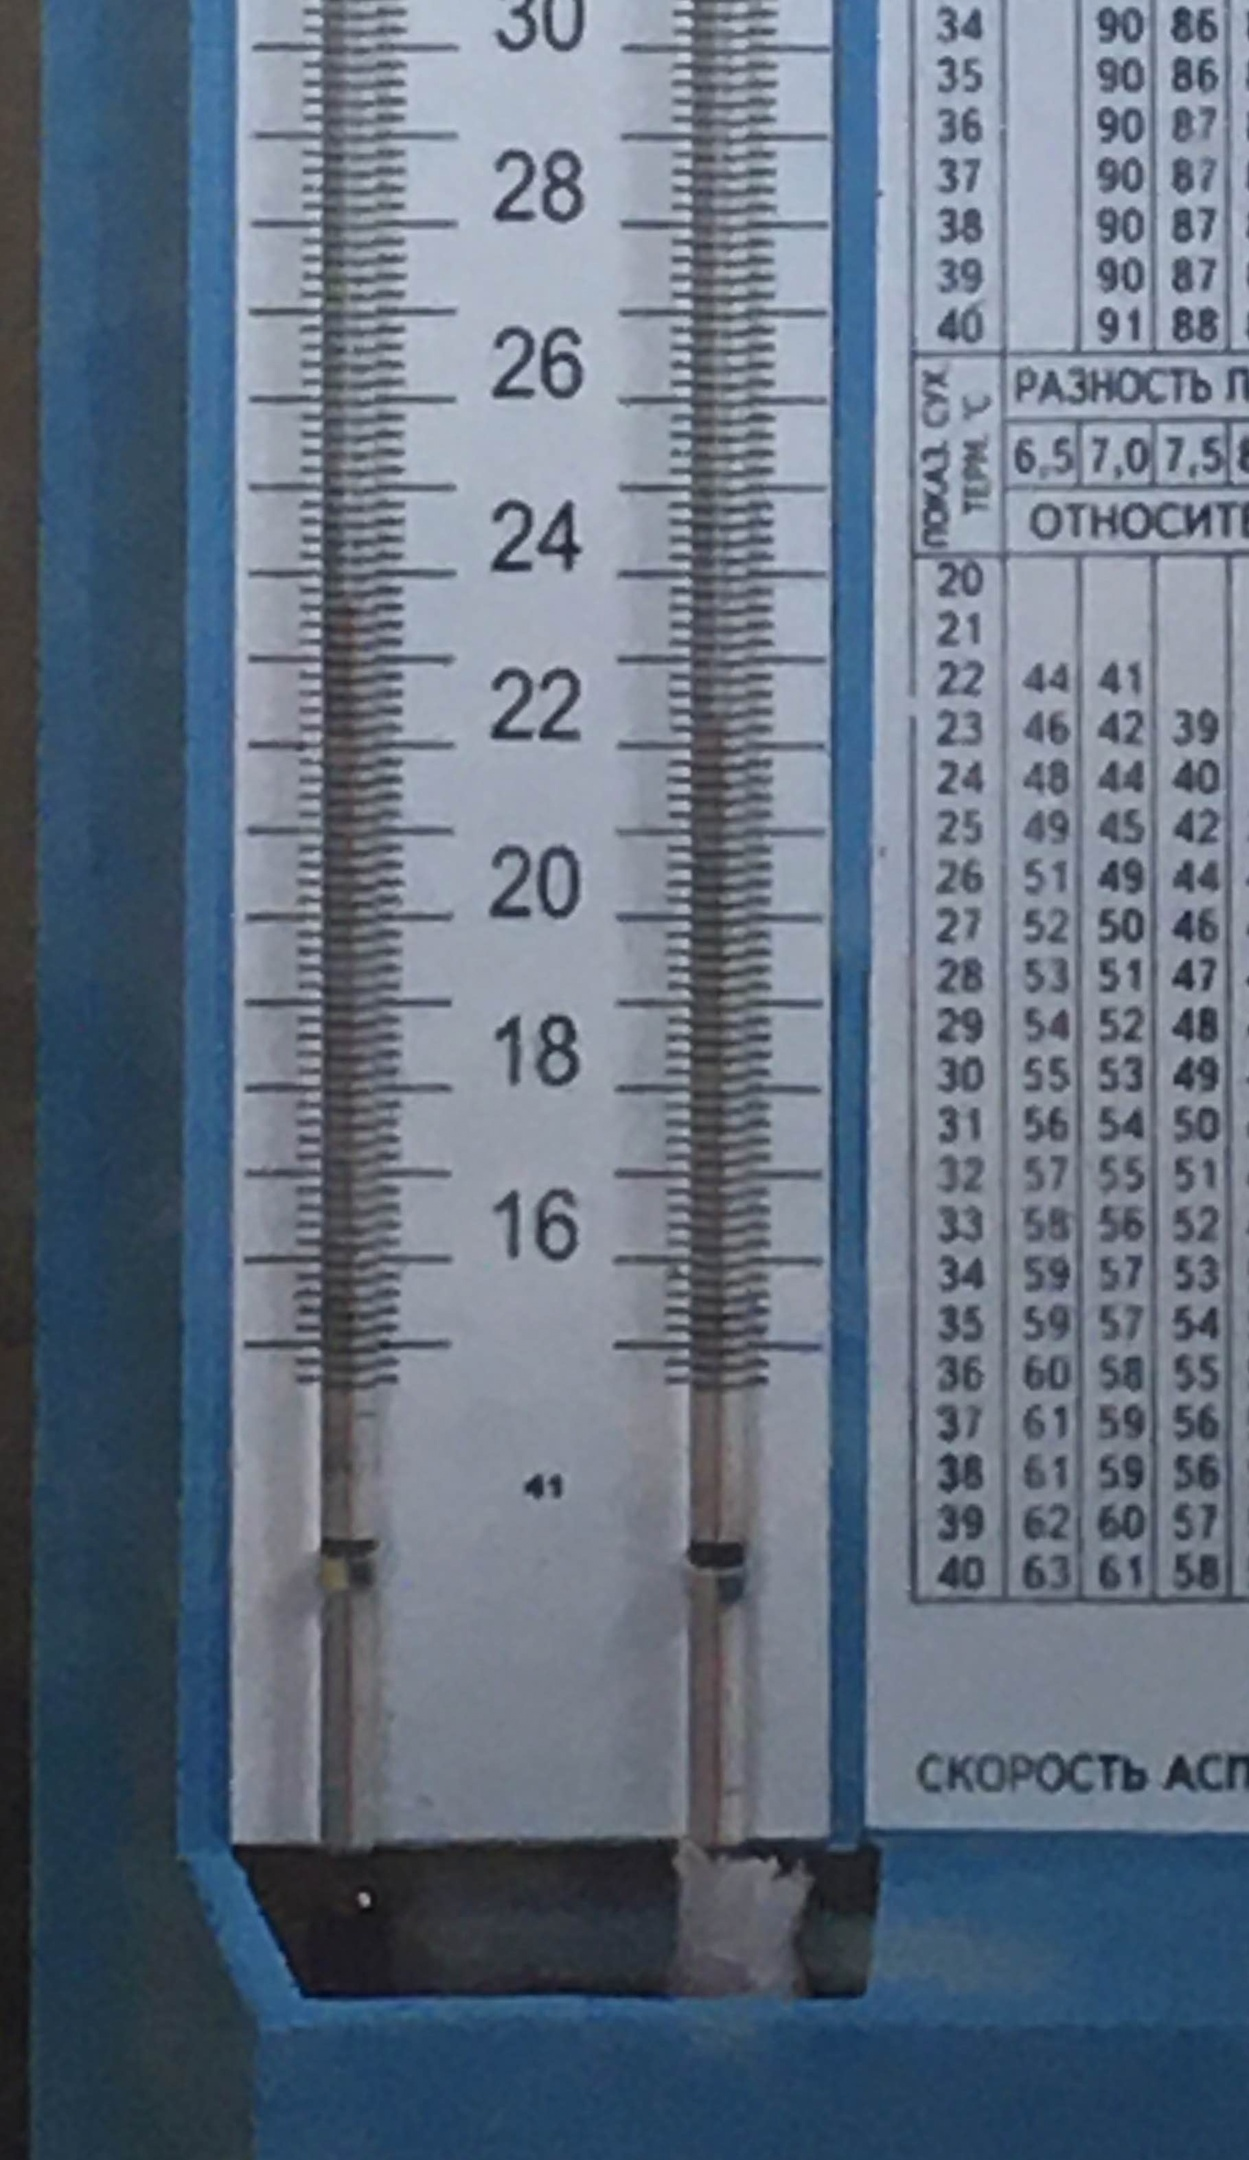
\includegraphics[width=40mm]{start.jpg}
&
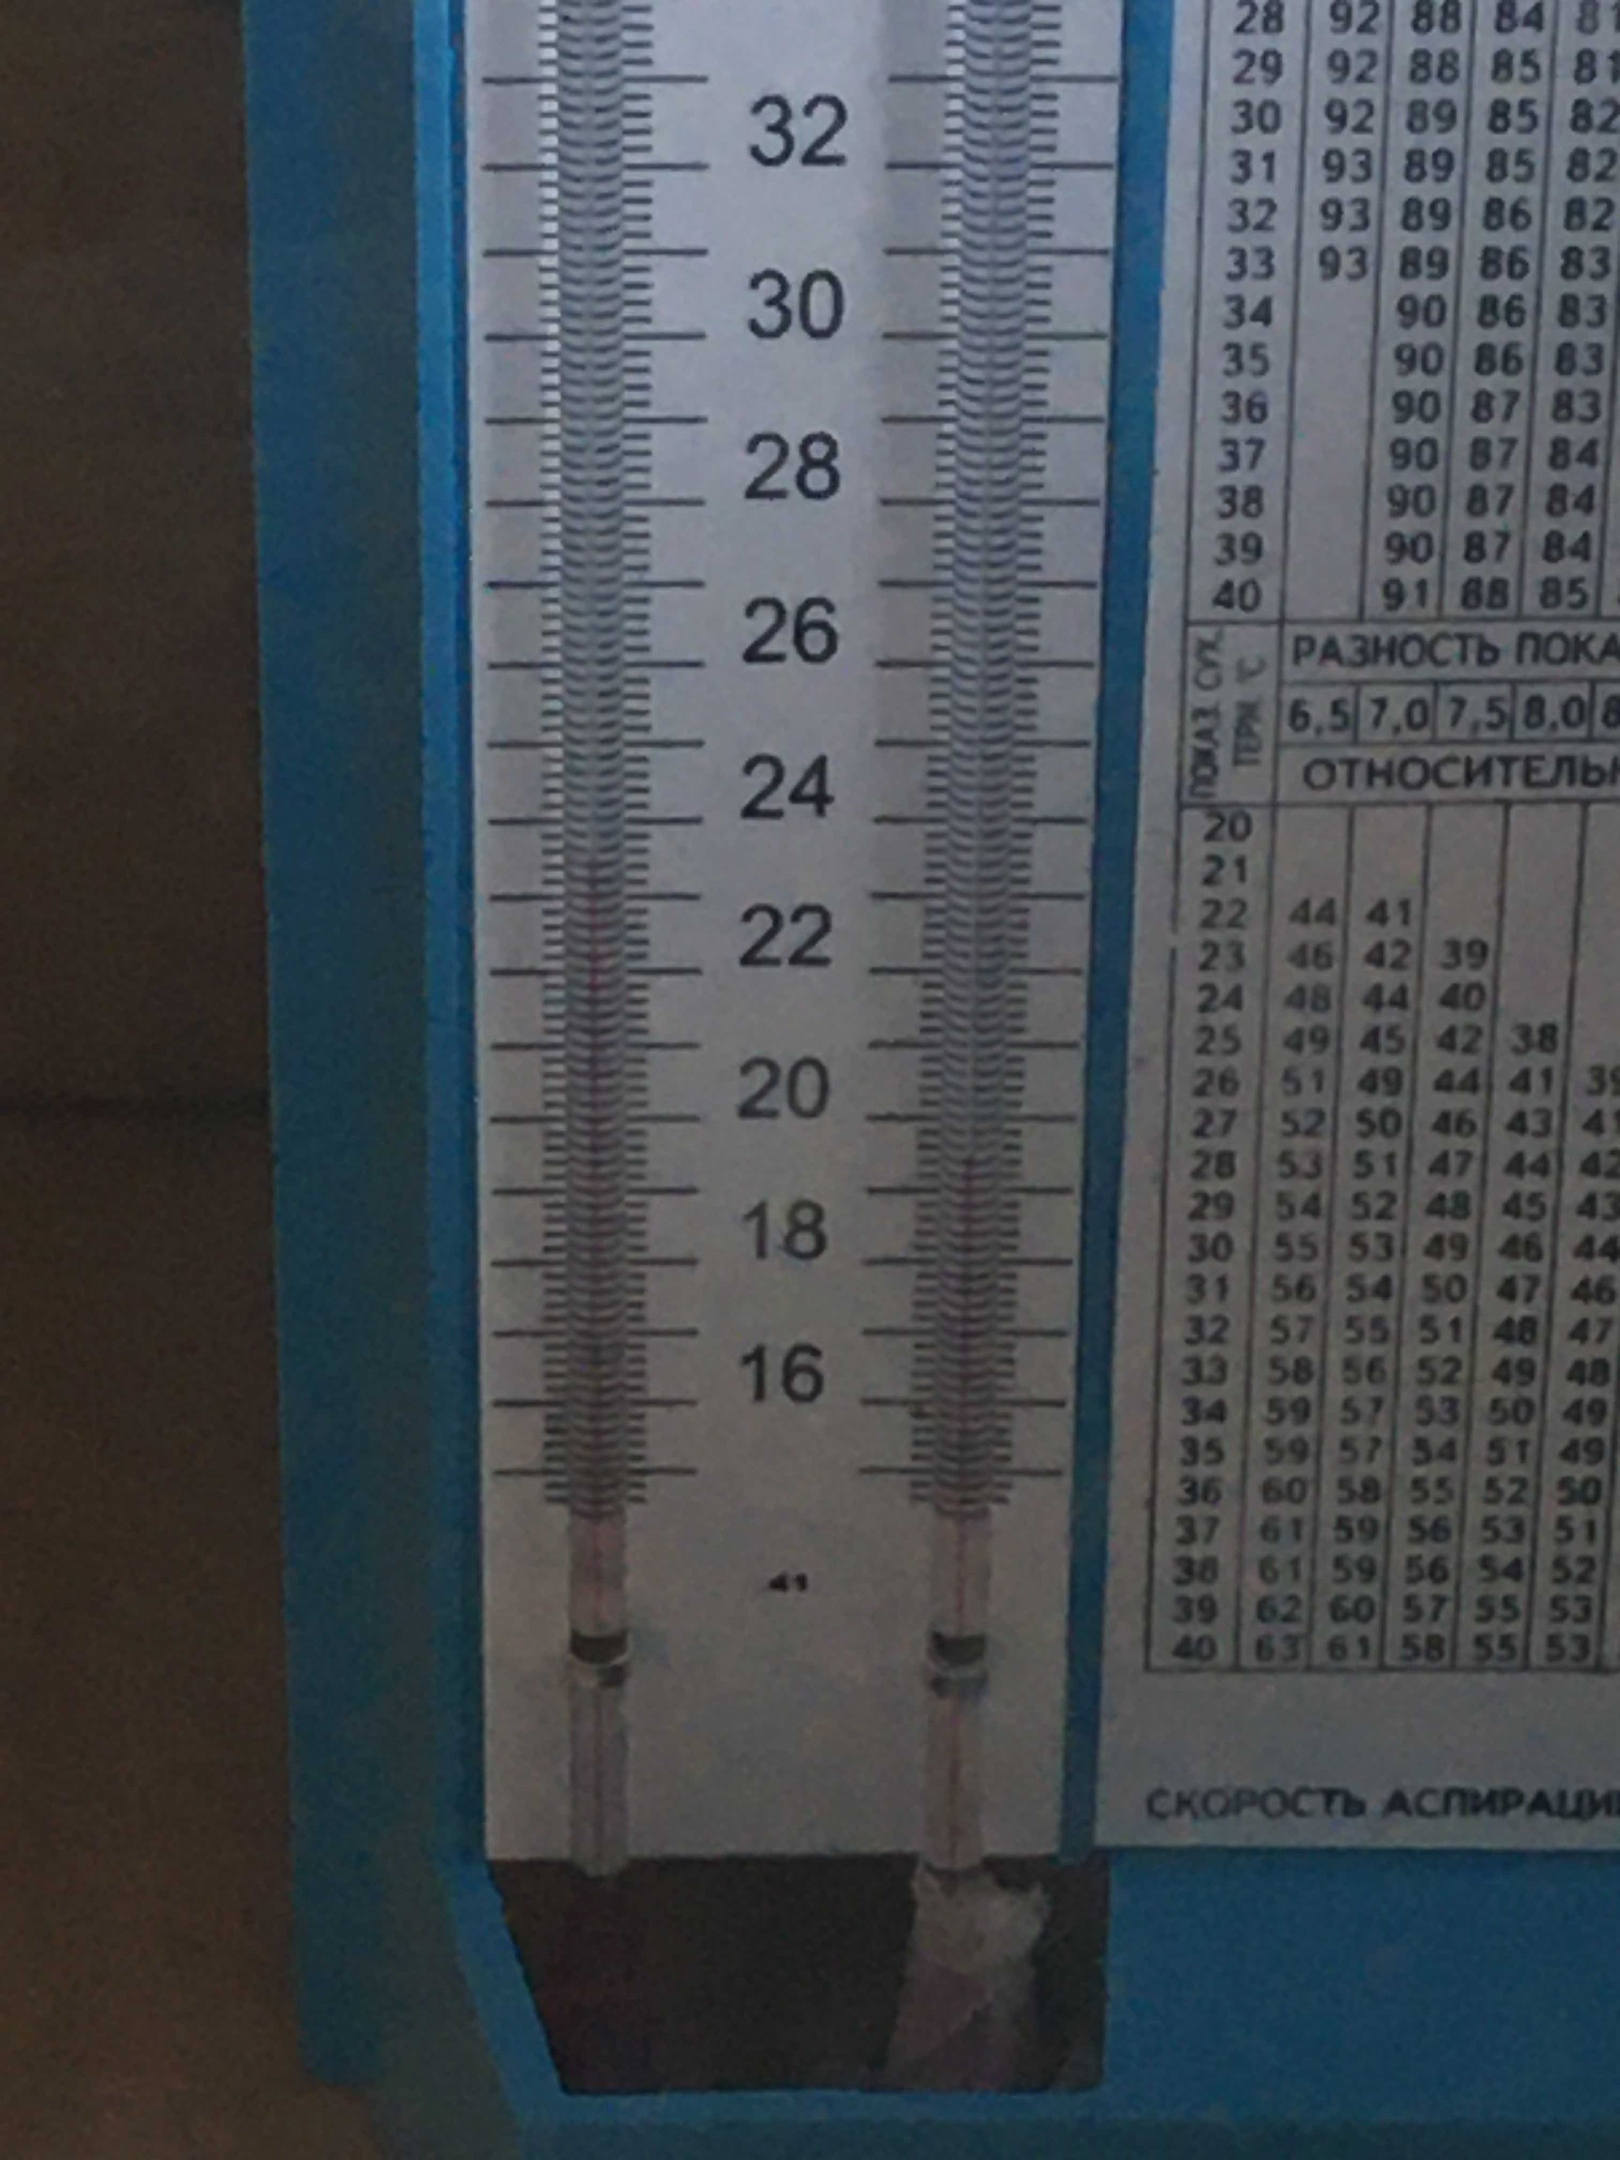
\includegraphics[width=51.8mm]{finish.jpg}
\end{tabular}
\caption{Состояния гигрометра в начале и в конце эксперимента}
\end{figure}

Оценим погрешность найденной величины (плотность - табличное значение, относительная влажность по психрометру постоянна в пределах одного-двух градусов, а погрешность температуры - пятая часть градуса, поэтому в финальную формулу решено было включить только измерения параметров помещения): $$\varepsilon = \sqrt{\left(\dfrac{\delta h}{h}\right)^2 + \left(\dfrac{\delta w}{w}\right)^2 + \left(\dfrac{\delta l}{l}\right)^2} = \sqrt{\left(\dfrac{0,005}{0,62}\right)^2 + \left(\dfrac{0,005}{0,51}\right)^2 + \left(\dfrac{0,005}{0,79}\right)^2} \approx 0,014 = 1,4\%.$$

\begin{figure}[ht]\center
\begin{tabular}{cc}
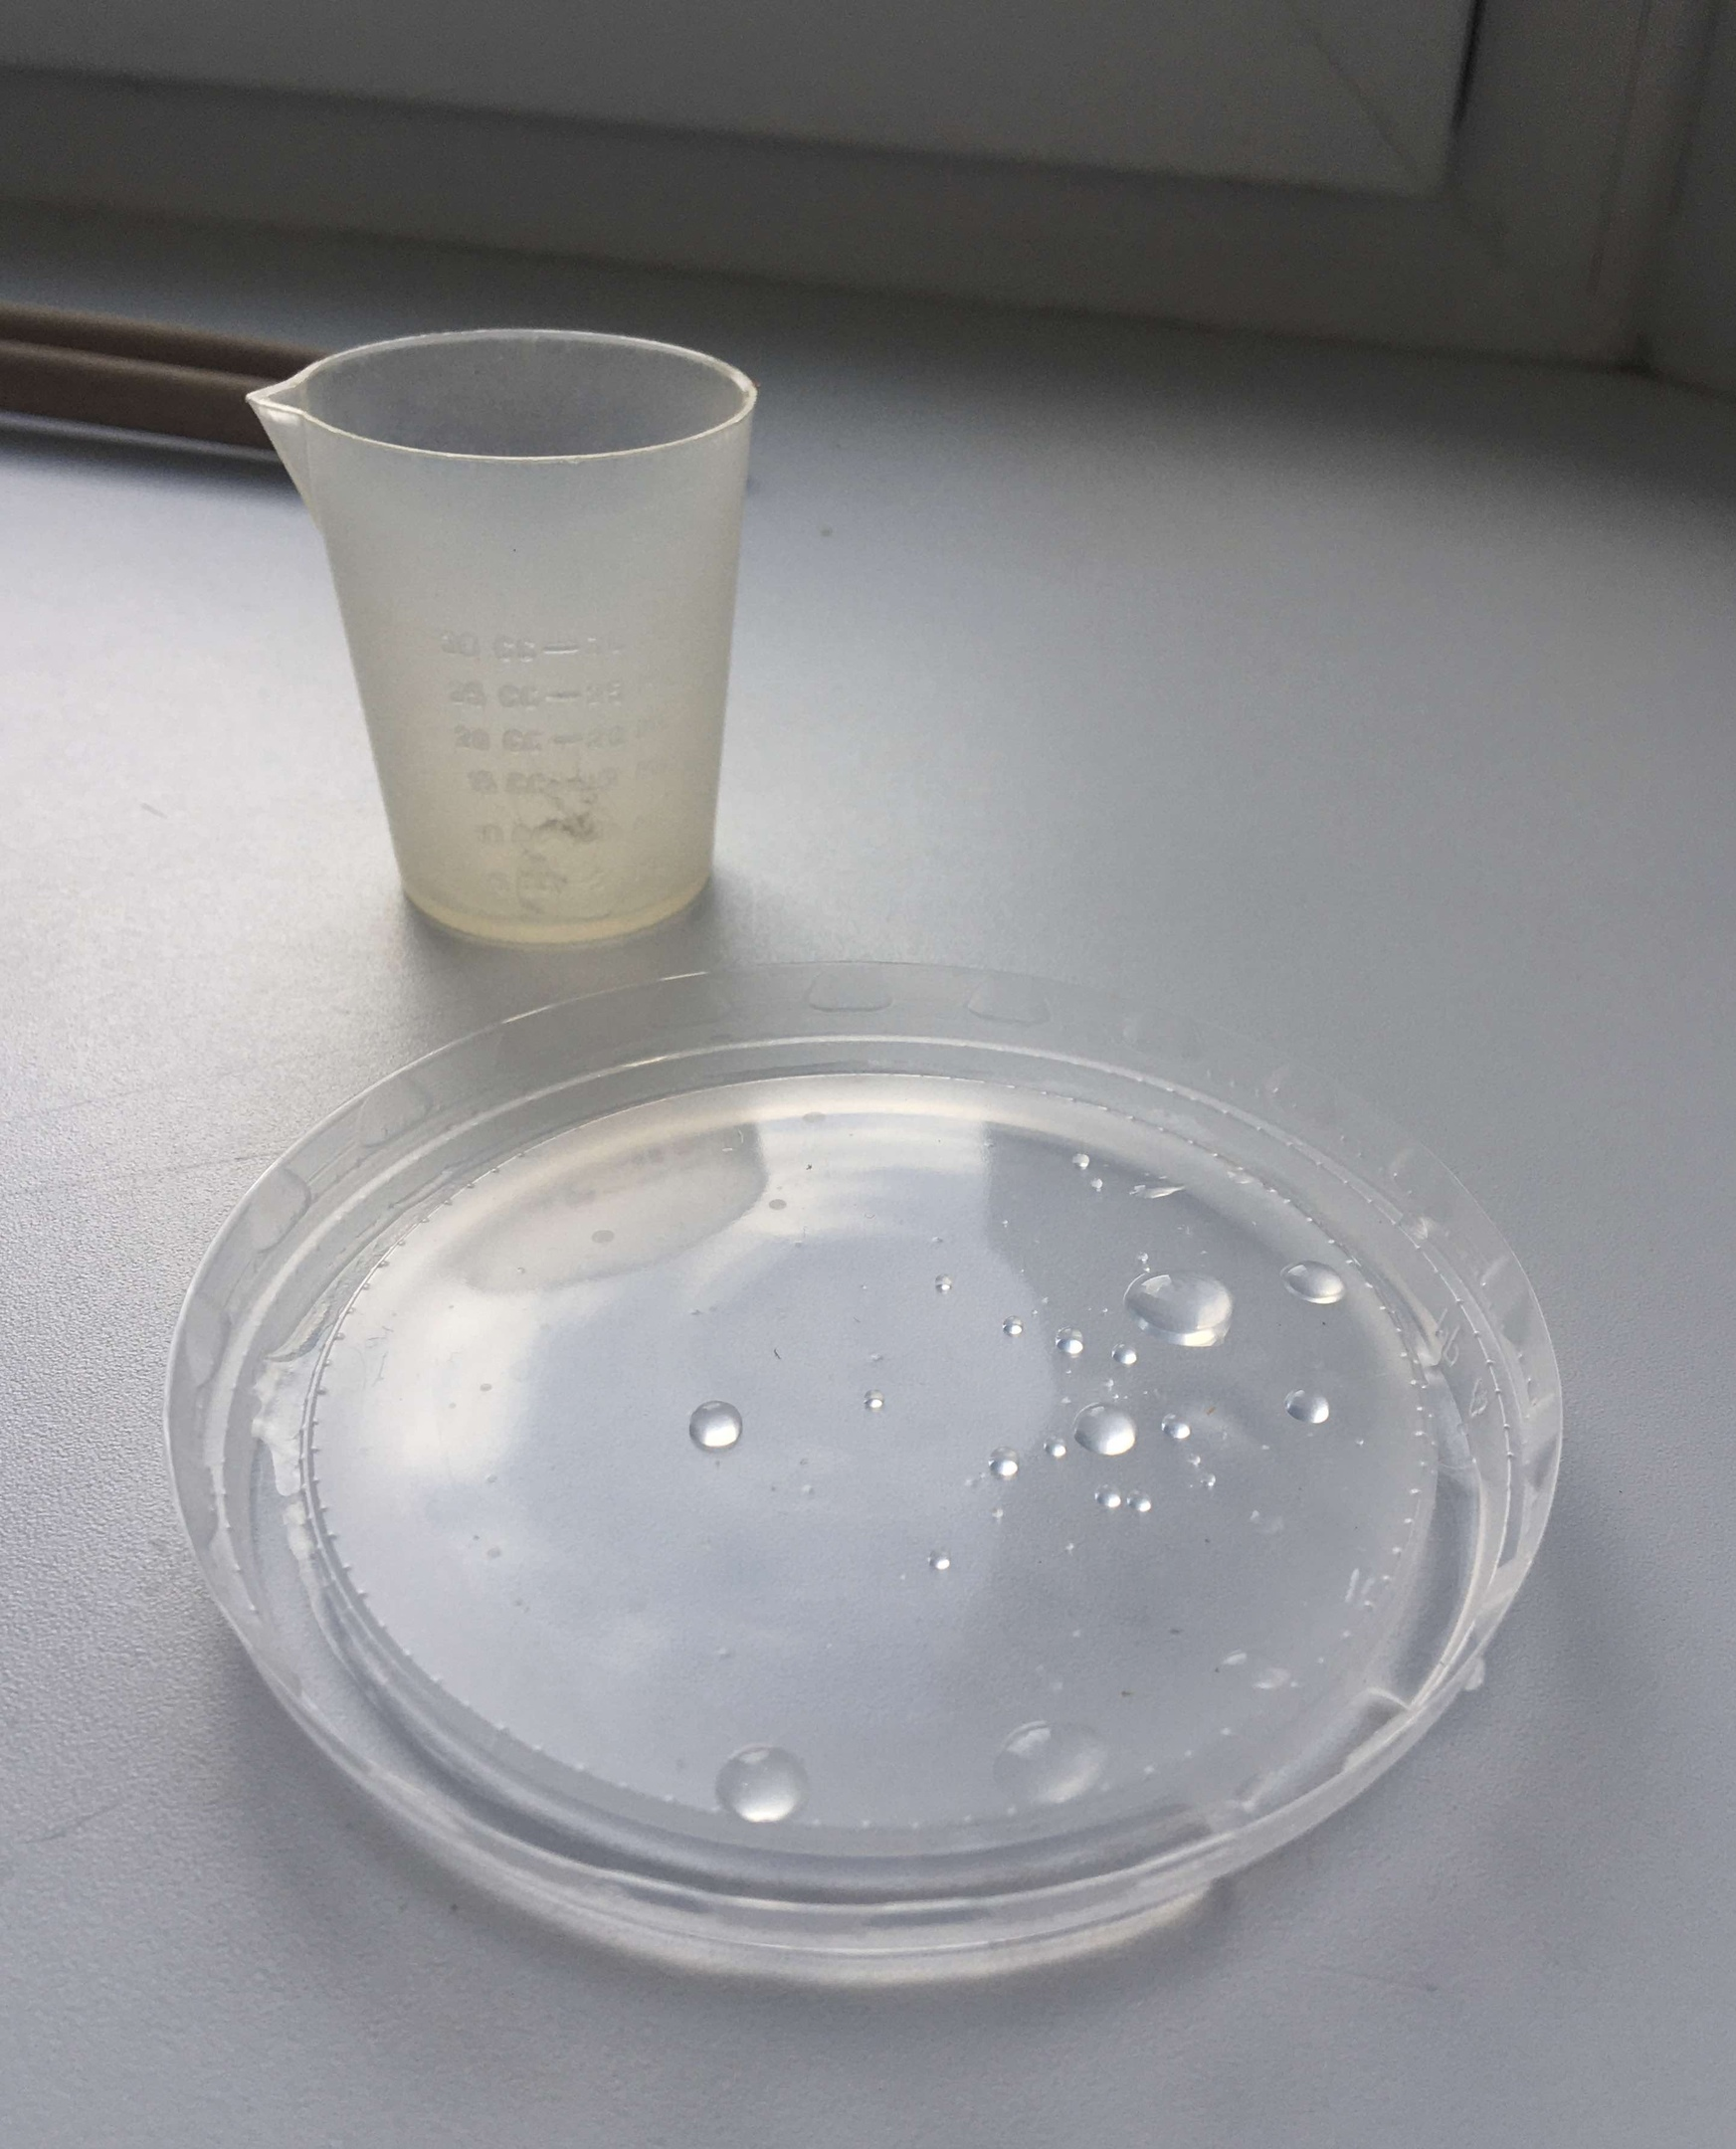
\includegraphics[width=65mm]{xexek.jpg}
&
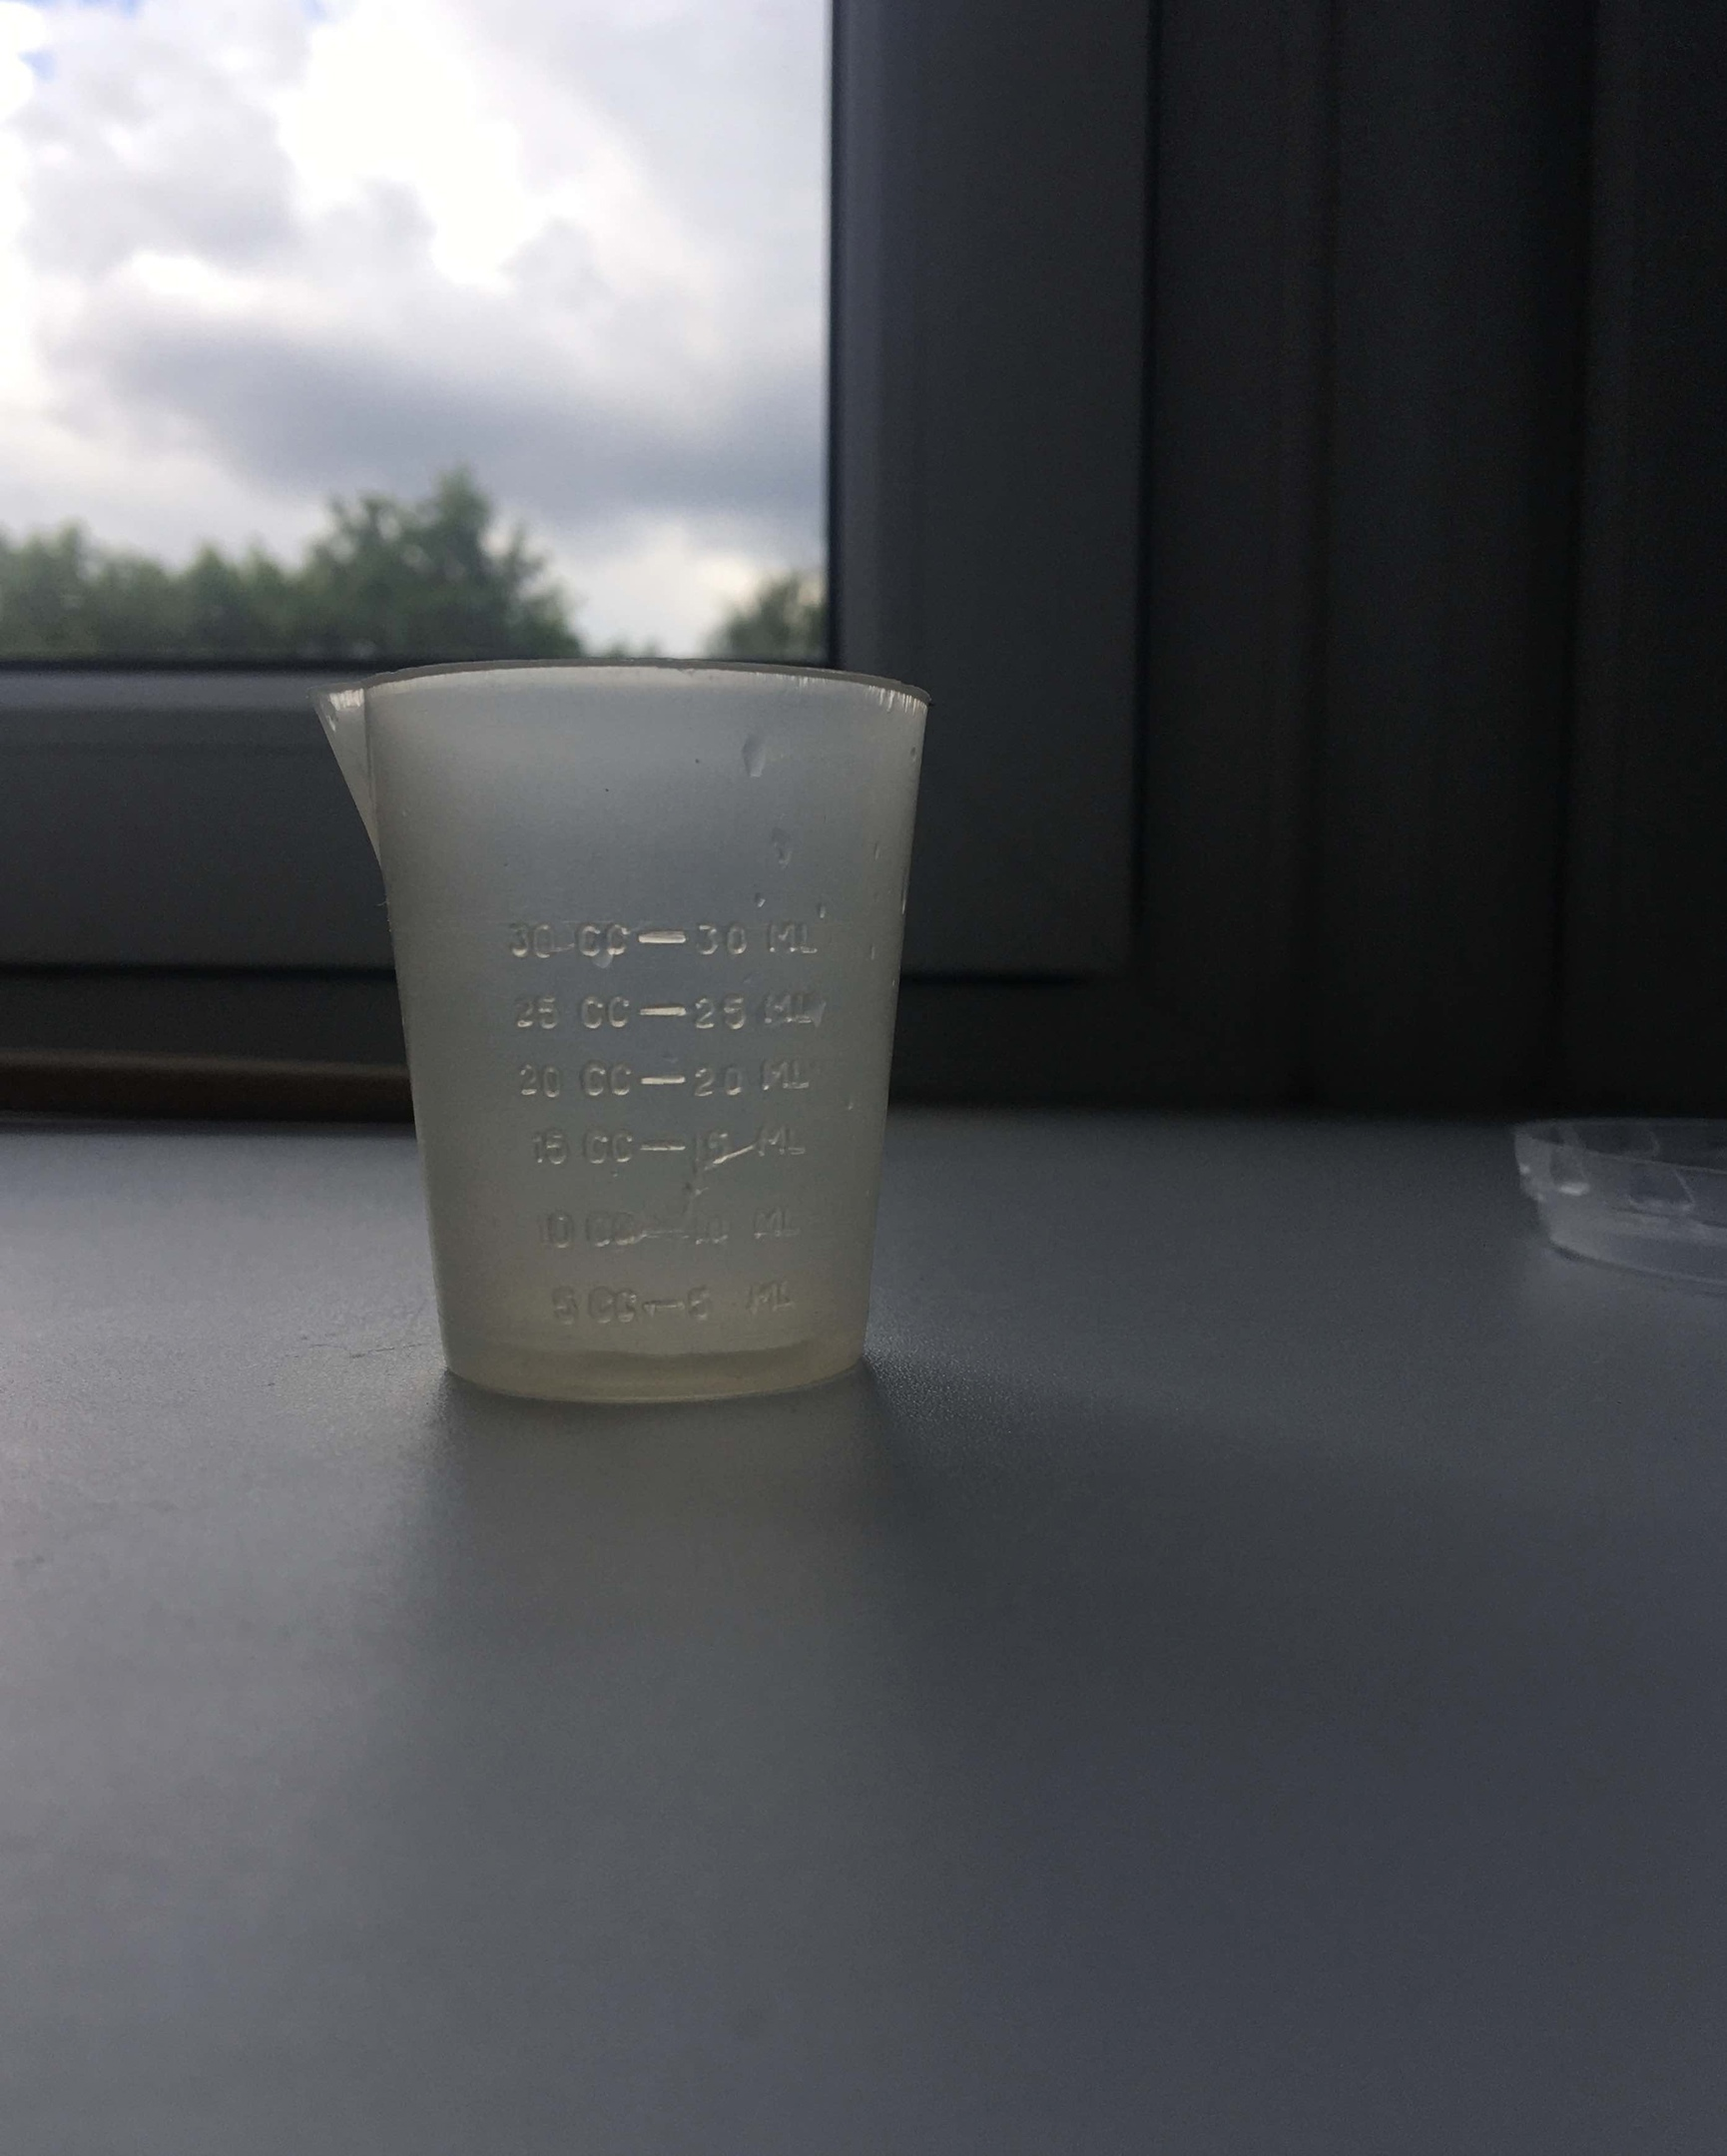
\includegraphics[width=65mm]{xexe.jpg}
\end{tabular}
\caption{Конденсат}
\end{figure}

На рис. 7 представлен конденсат. На фото справа он перелит из ёмкости для сбора жидкости в измерительный стакан. Практическое значение $\Delta v \approx$ 2 мл (погрешность можно оценить лишь условно в пределах точности глазомера ($\pm$ 0,5 мл), так как цена деления измерительного стакана больше объёма конденсата), что примерно в полтора раза превышает численную оценку. Это обусловлено недостаточной герметичностью коробки и техническими несовершенствами установки, поэтому вследствие проникновения новых порций воздуха в выбранный объем истинная величина сконденсировавшейся воды оказалась выше.


\newpage

%6
%=======================================================================================

\section{Идеи для дальнейшего исследования}
При работе осушителя влажность помещения падает. В теории, при стремлении времени к бесконечности концентрация водяных паров в помещении сравняется с концентрацией насыщенного пара при температуре, равной температуре на холодном радиаторе.

Обозначим $n_0, T_0$ концентрацию и температуру в помещении и $T_1$ --- температуру на холодном радиаторе установки. Пусть $n_1$ --- концентрация насыщенных паров при $T_1$. Пусть также $t$ --- время эксперимента. Тогда:
$$\lim\limits_{t \to \infty} n_0 = n_1$$
Как уже отмечалось, изоляция установки от внешних факторов далека от идеала, и время снижения показаний влажности в исследовании, рассмотренном выше, замедлялось с каждым делением, поэтому для проверки этого предположения в данных условиях продолжительность эксперимента надо было и вправду устремить к бесконечности, так как разность температур и, соответственно, концентраций велика относительно уловий опыта. Конструкция аппарата, мощность осушителя и недостаточное количество времени не позволили бы проанализировать данное соотношение, поэтому в перспективе можно подумать над принципиальным улучшением герметичности помещения и об увеличении количества элементов Пельтье для создания целой системы осушителей с целью расширения площади поверхности для образования конденсата и модернизации эффективности осушения фиксированного объёма воздуха.

\newpage

%7
%=======================================================================================

\section{Источники и ресурсы}

1. Вестник науки Сибири. 2015. Спецвыпуск (15)

2. https://usamodelkina.ru/11693-samodelnyj-osushitel-vozduha-na-jelemente-pelte.html

3. https://ventkam.ru/vozduh/osushenie/element-pelte

4. http://mypractic.ru/element-pelte-tec1-12706-xarakteristiki-primenenie-usloviya-ekspluatacii.html


\newpage

%8
%=======================================================================================

\section{Приложение}

\begin{figure}[h!]
	\begin{minipage}[h]{0.5\linewidth}
		\center{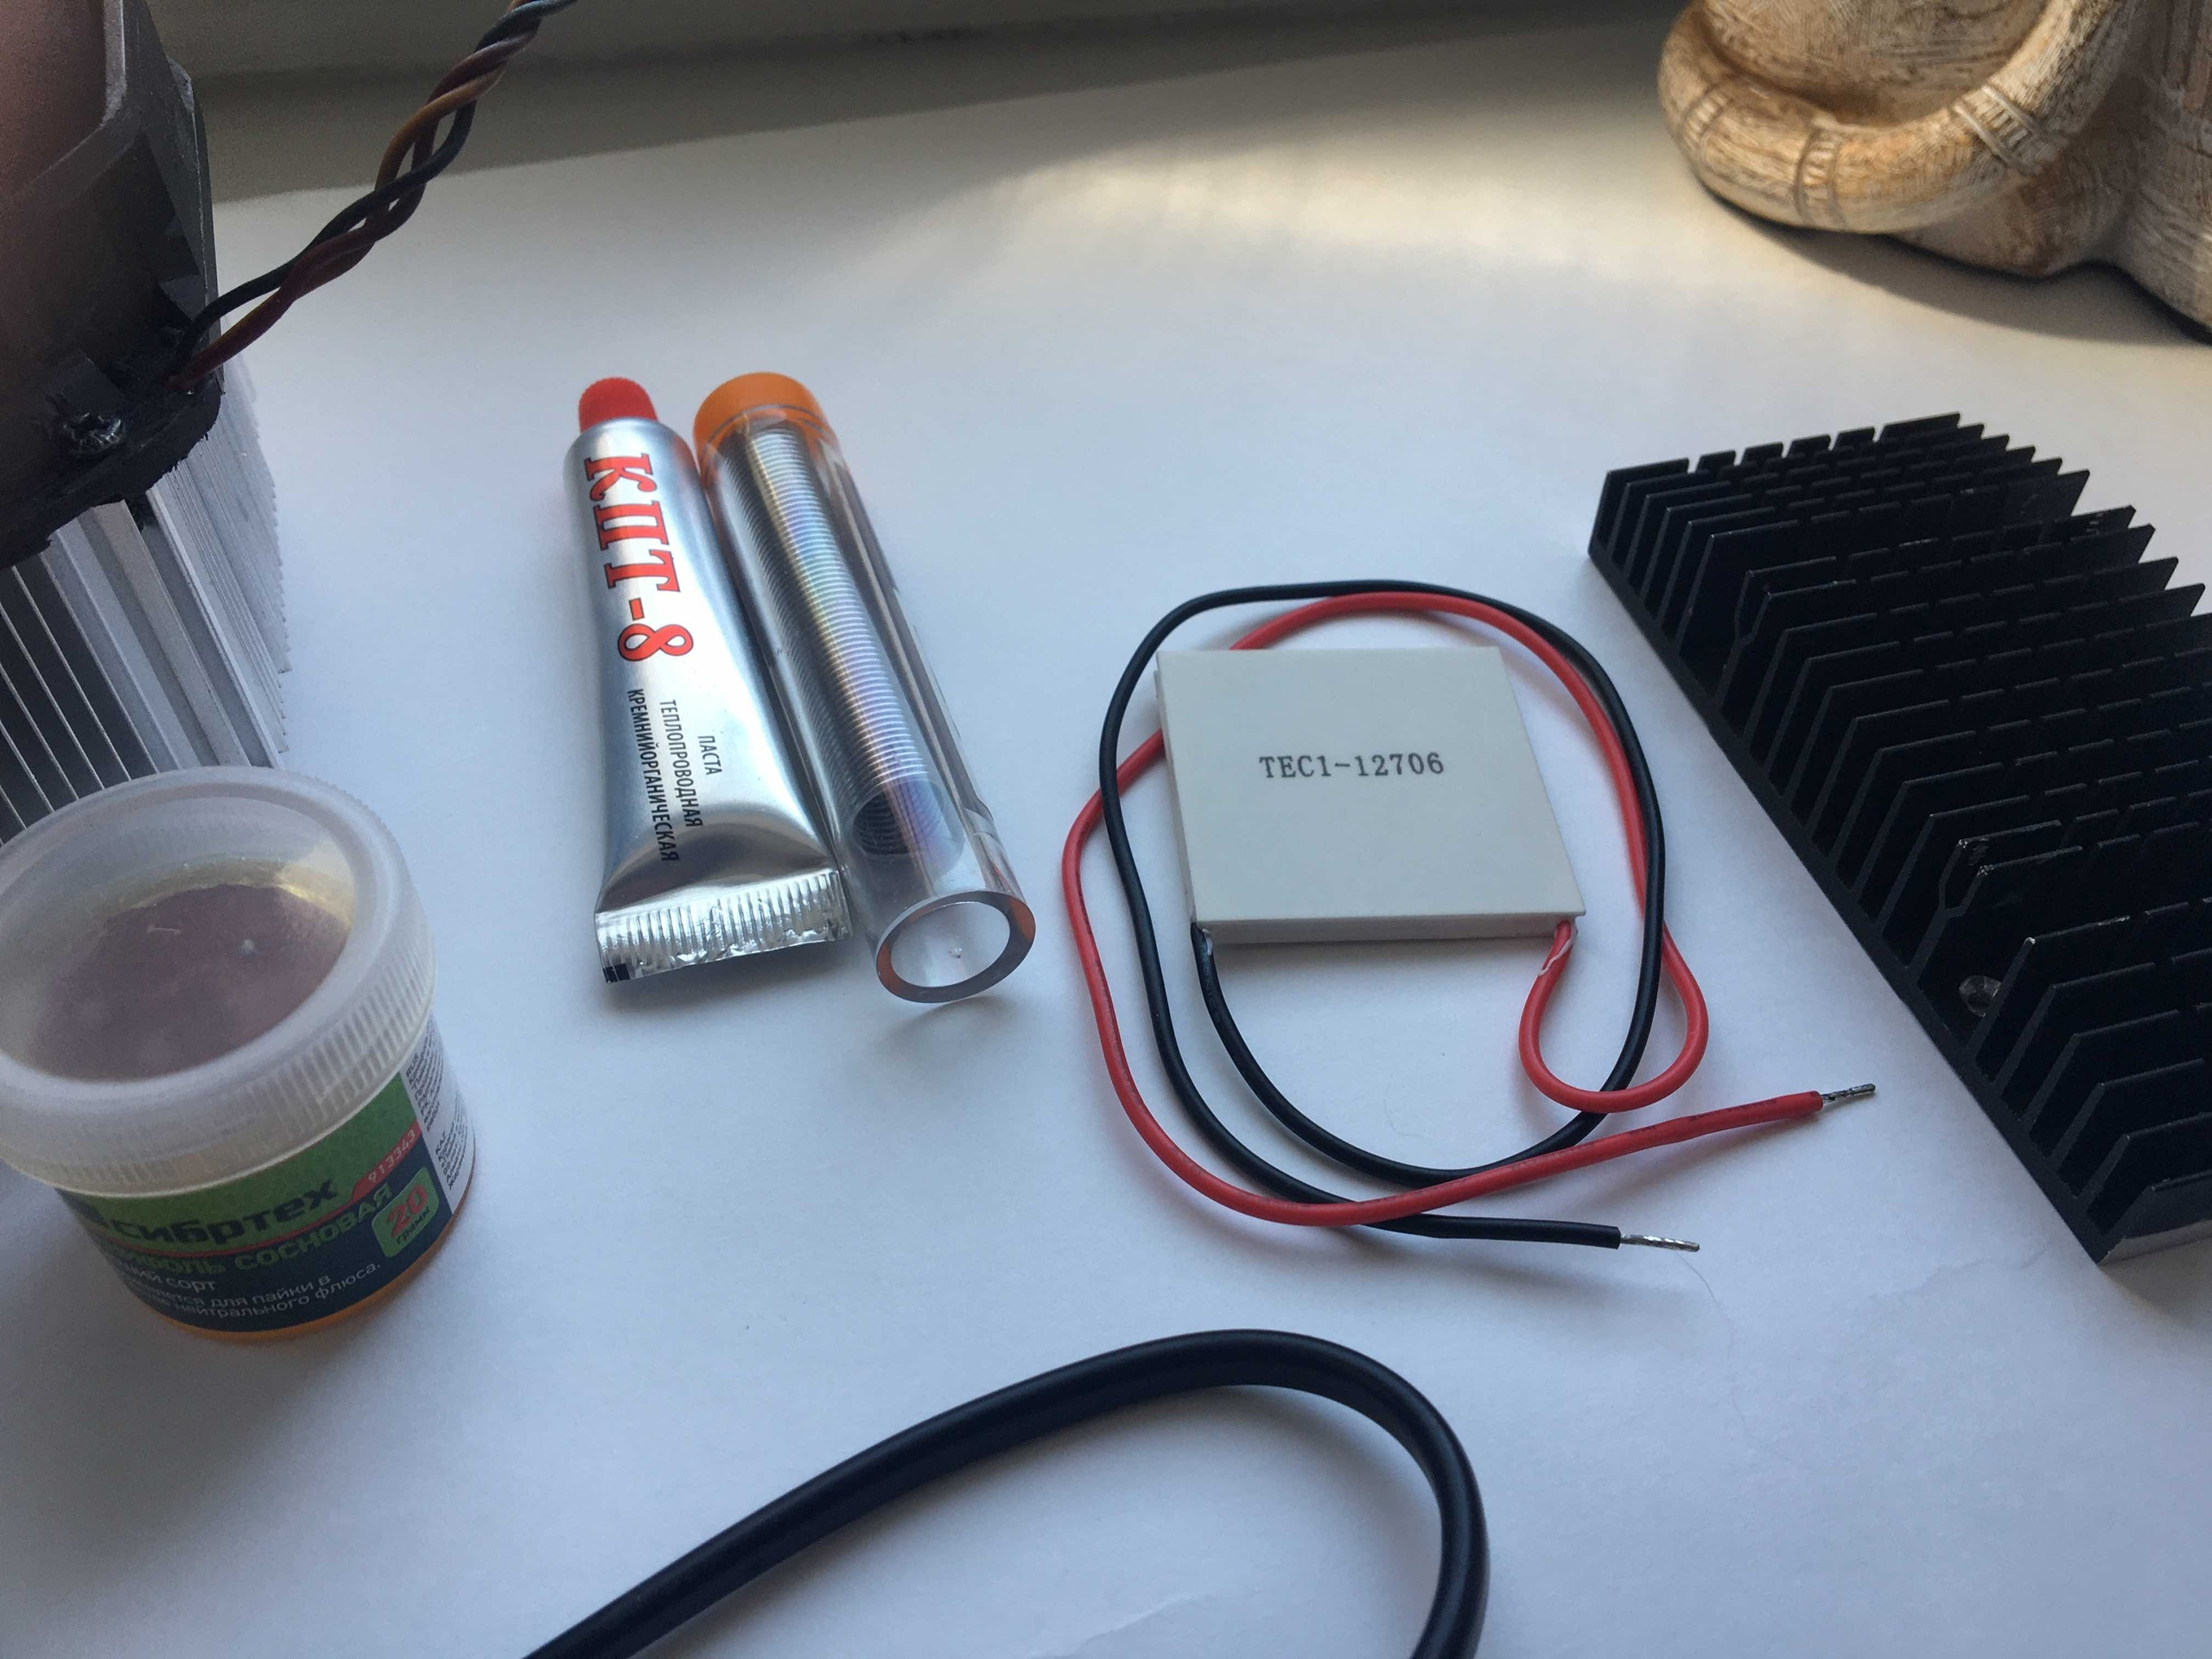
\includegraphics[width = 80mm]{pelt.jpg} \\ Элемент Пельтье}
	\end{minipage}
	\hfill
	\begin{minipage}[h]{0.5\linewidth}
		\center{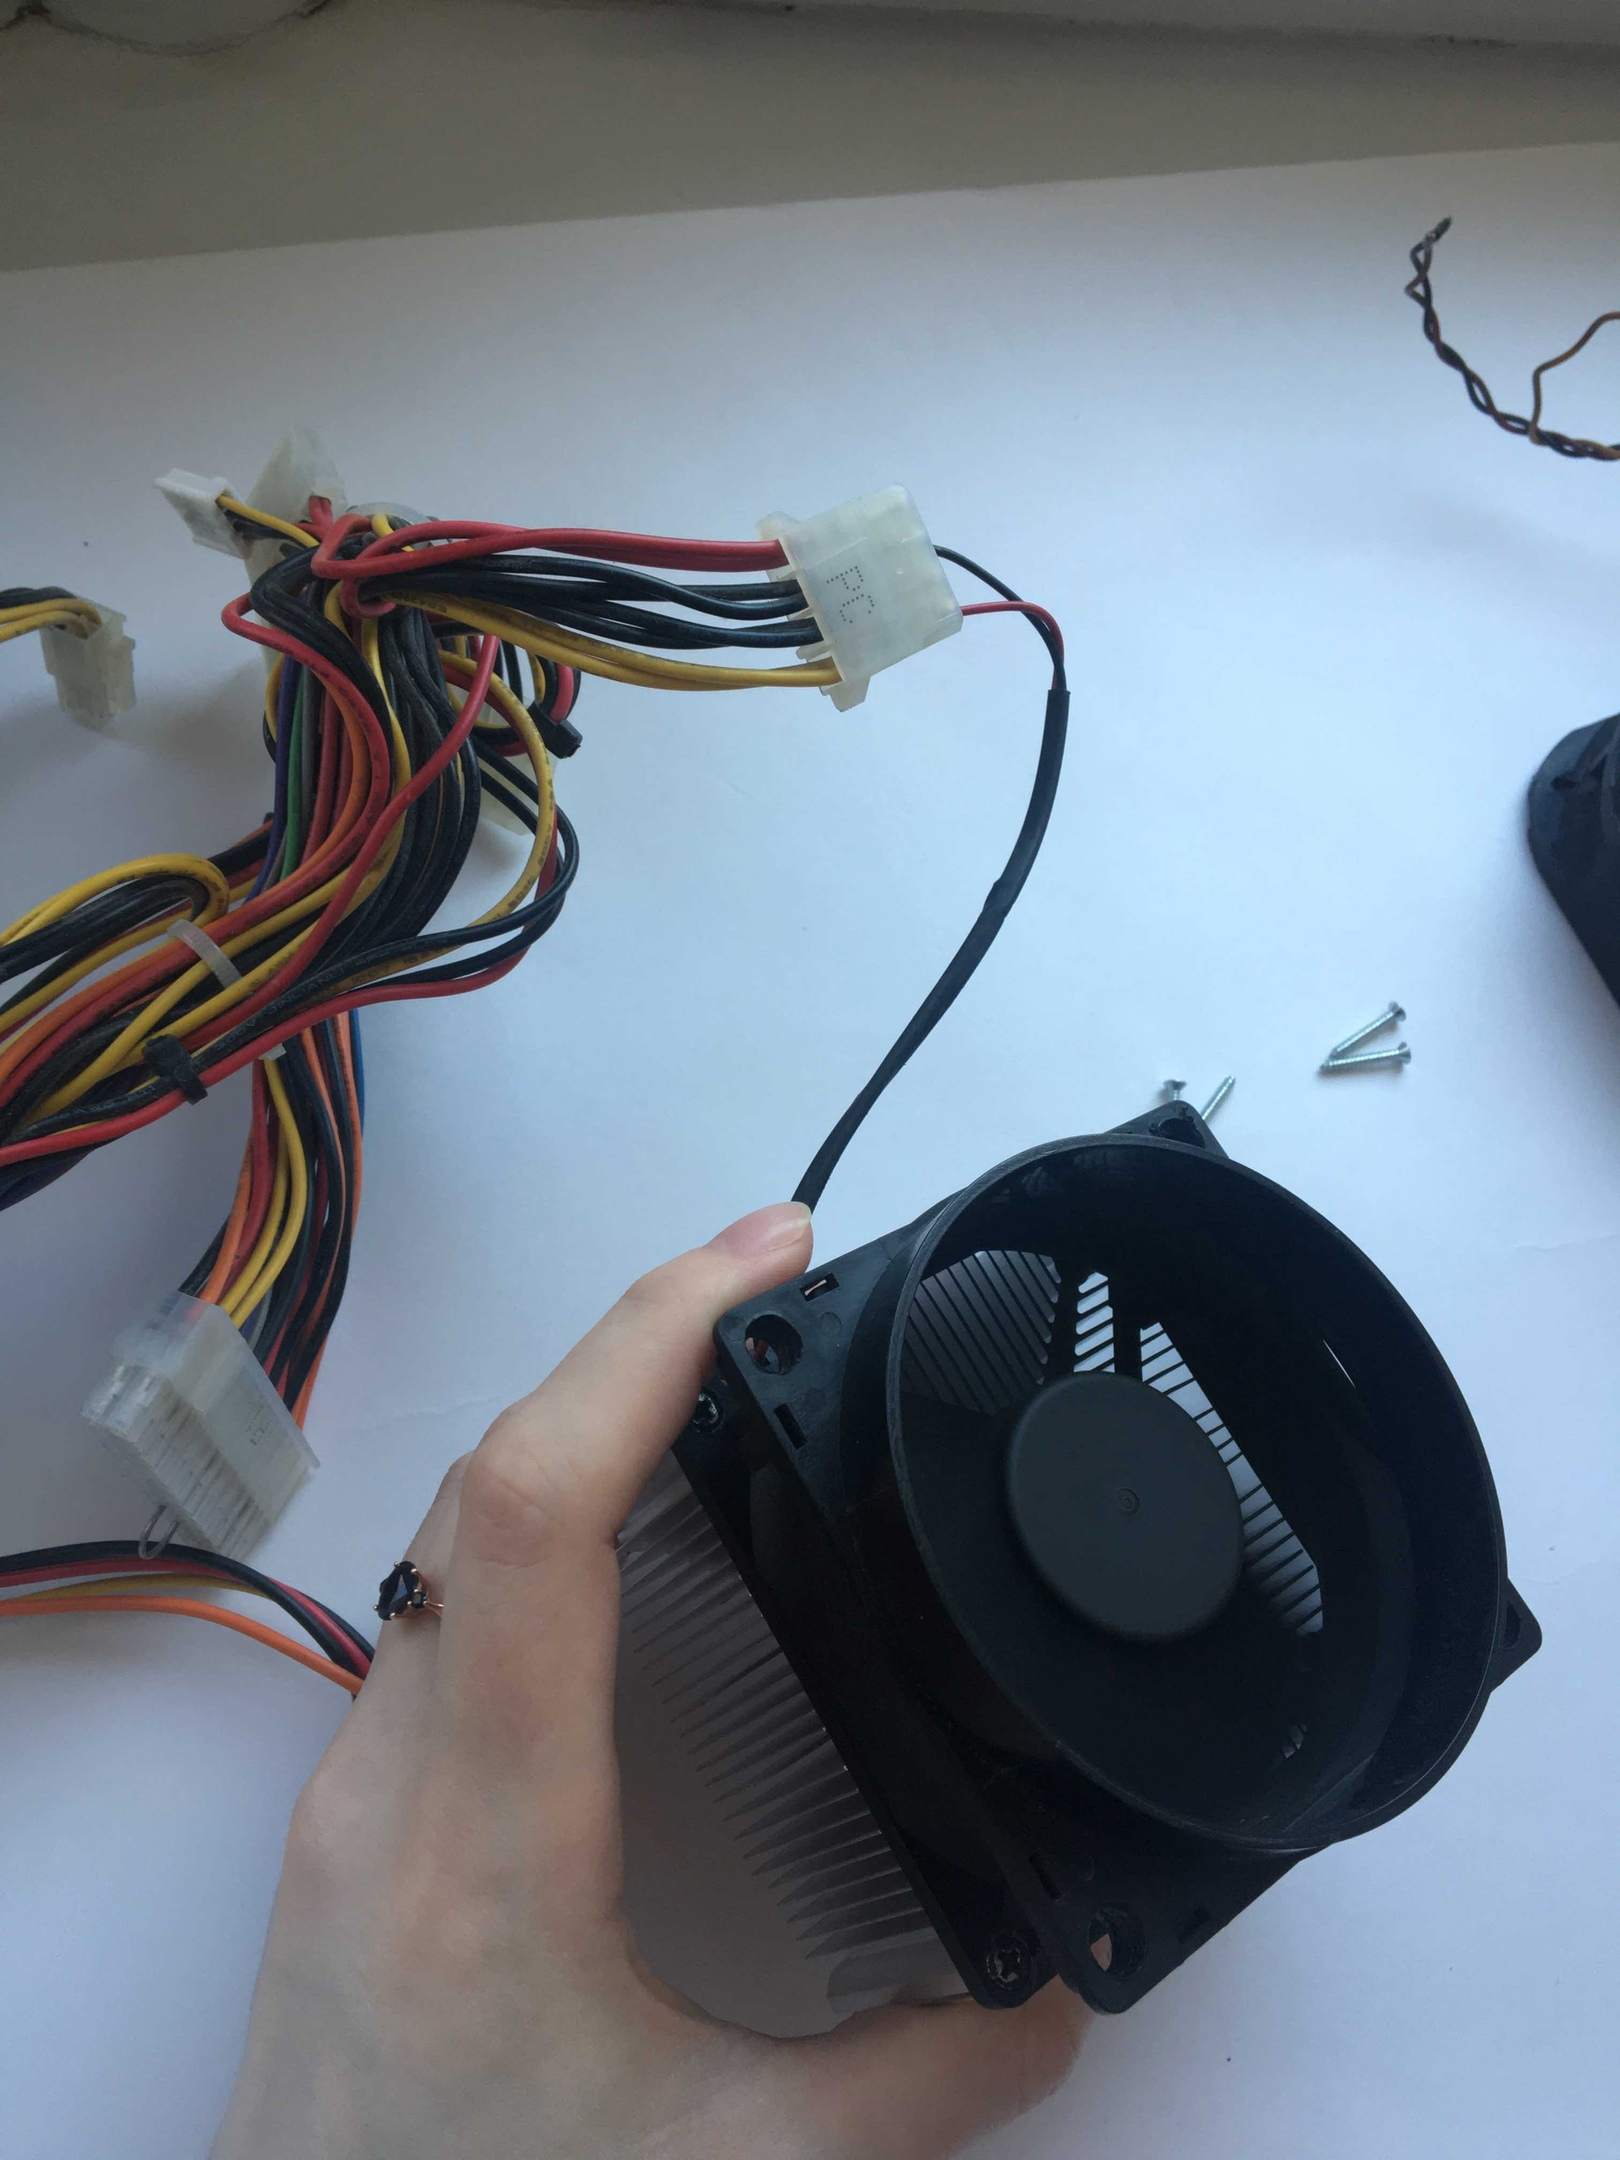
\includegraphics[width = 65mm]{sbor.jpg} \\ Сборка}
	\end{minipage}
\end{figure}

\begin{figure}[h!]
	\begin{minipage}[h]{0.5\linewidth}
		\center{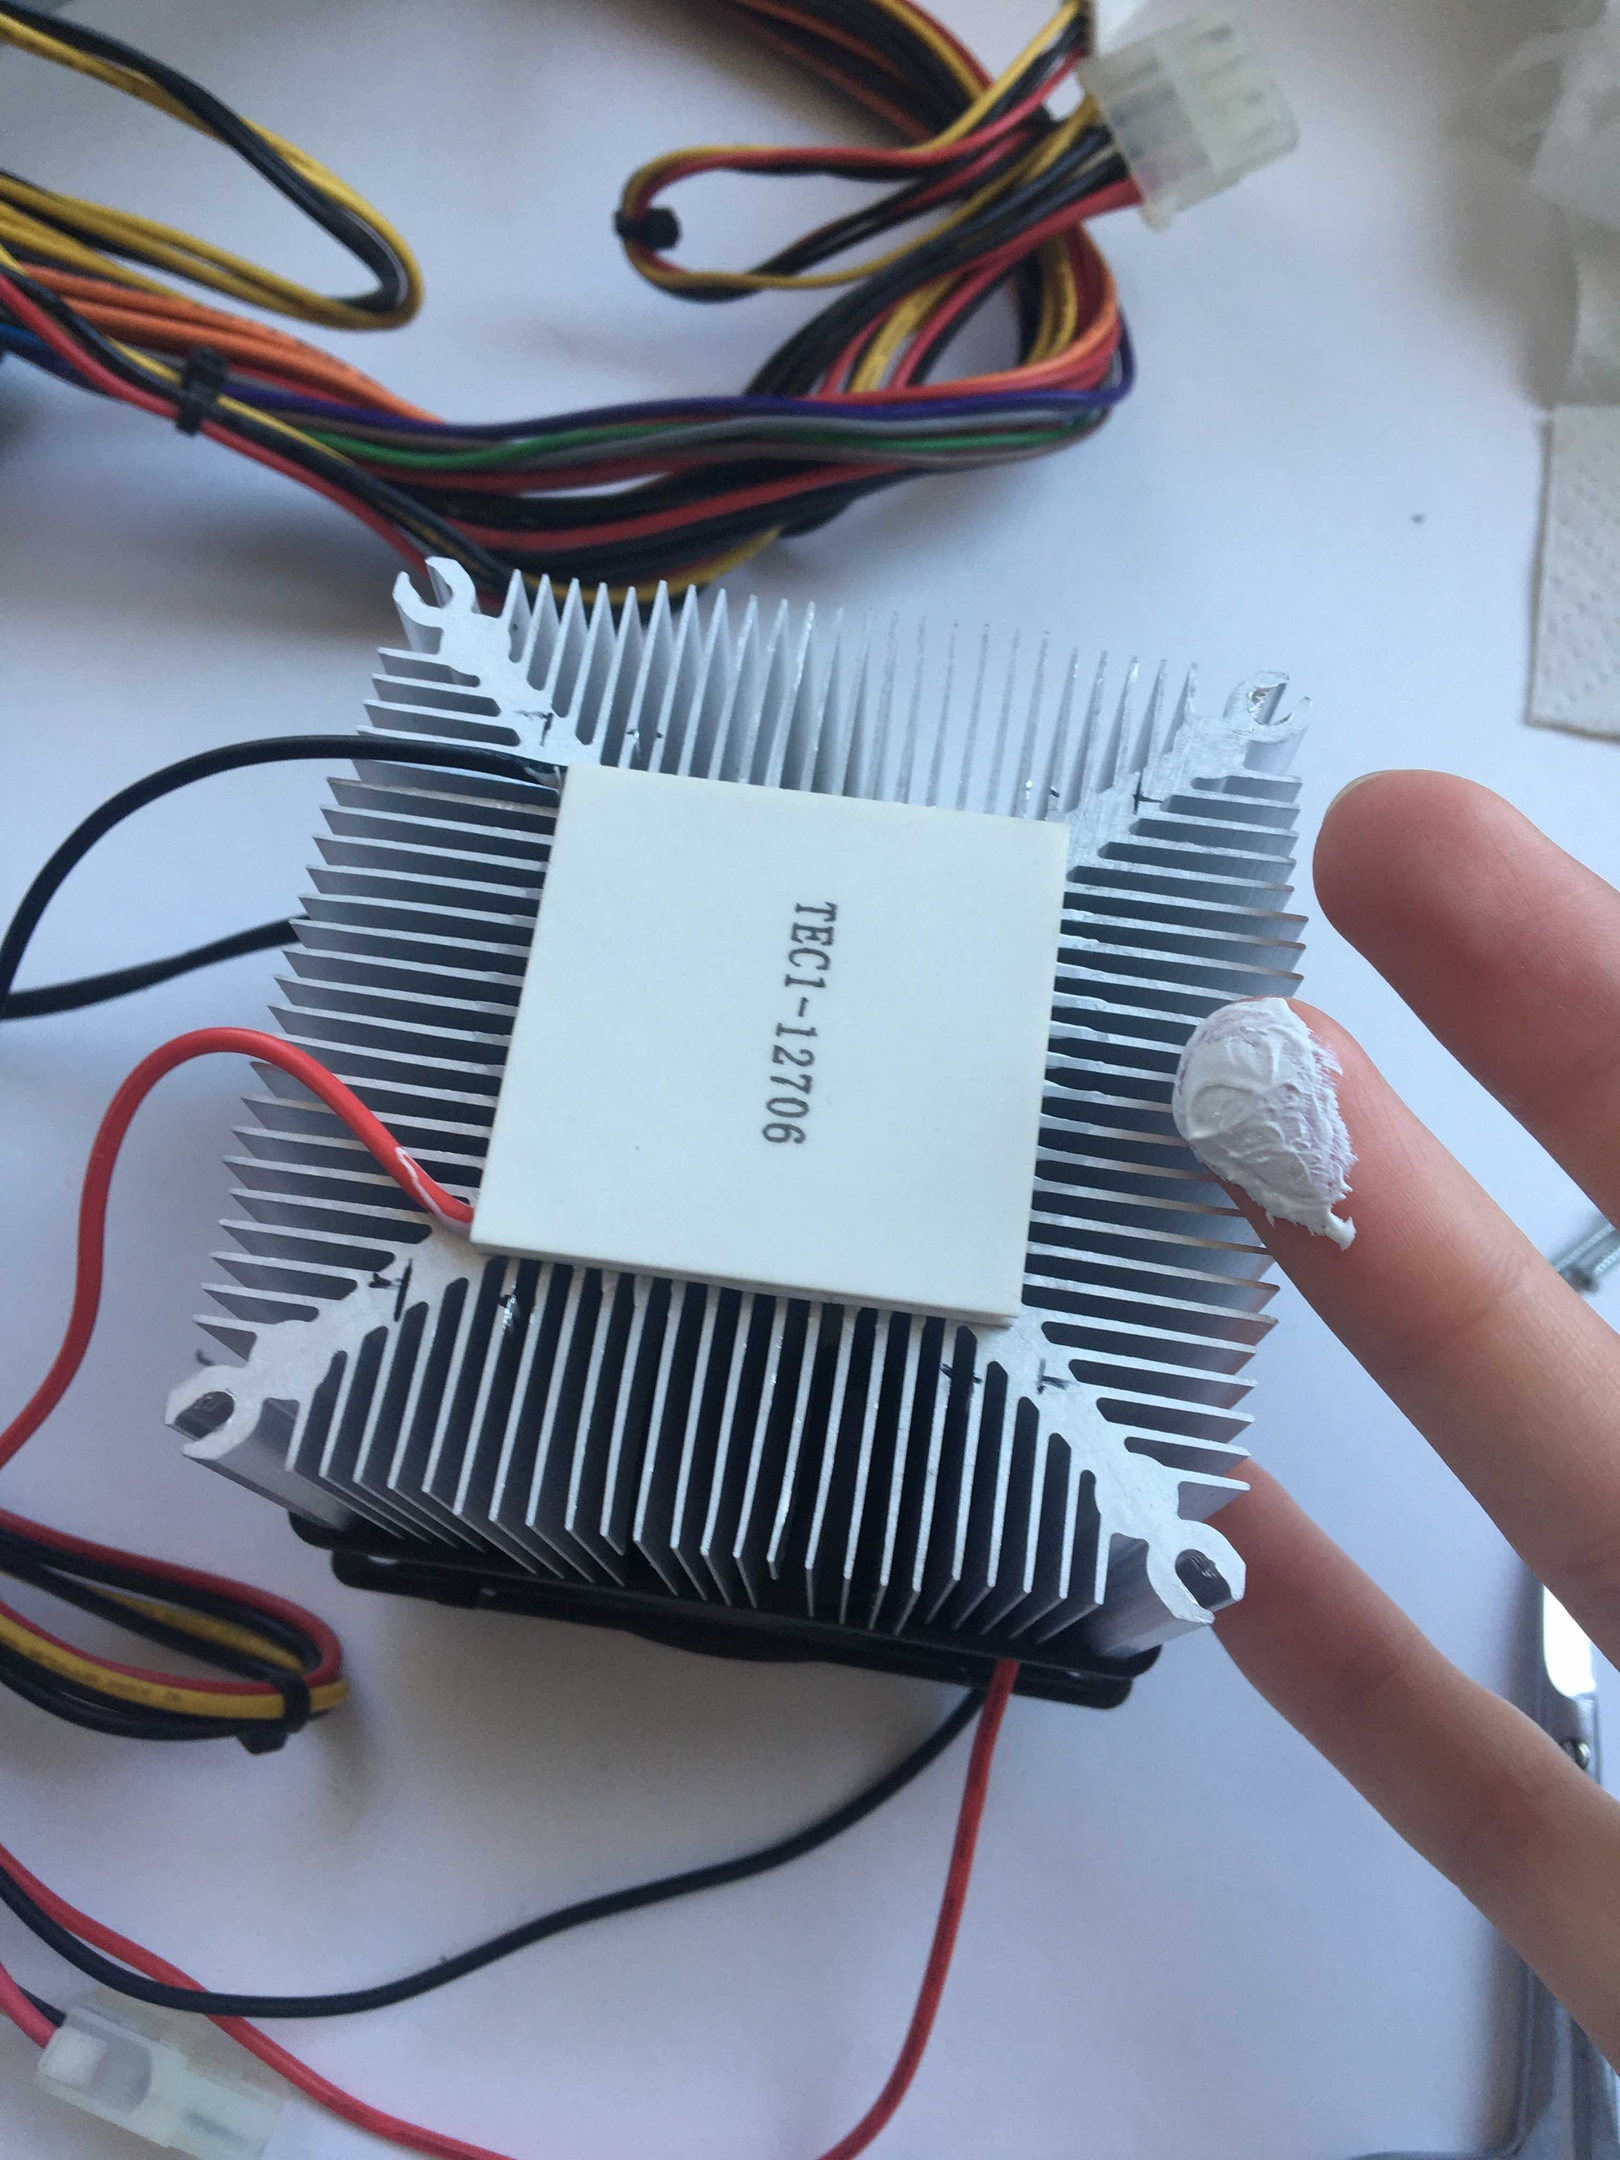
\includegraphics[width = 80mm]{pasta.jpg} \\ Нанесение термопасты}
	\end{minipage}
	\hfill
	\begin{minipage}[h]{0.5\linewidth}
		\center{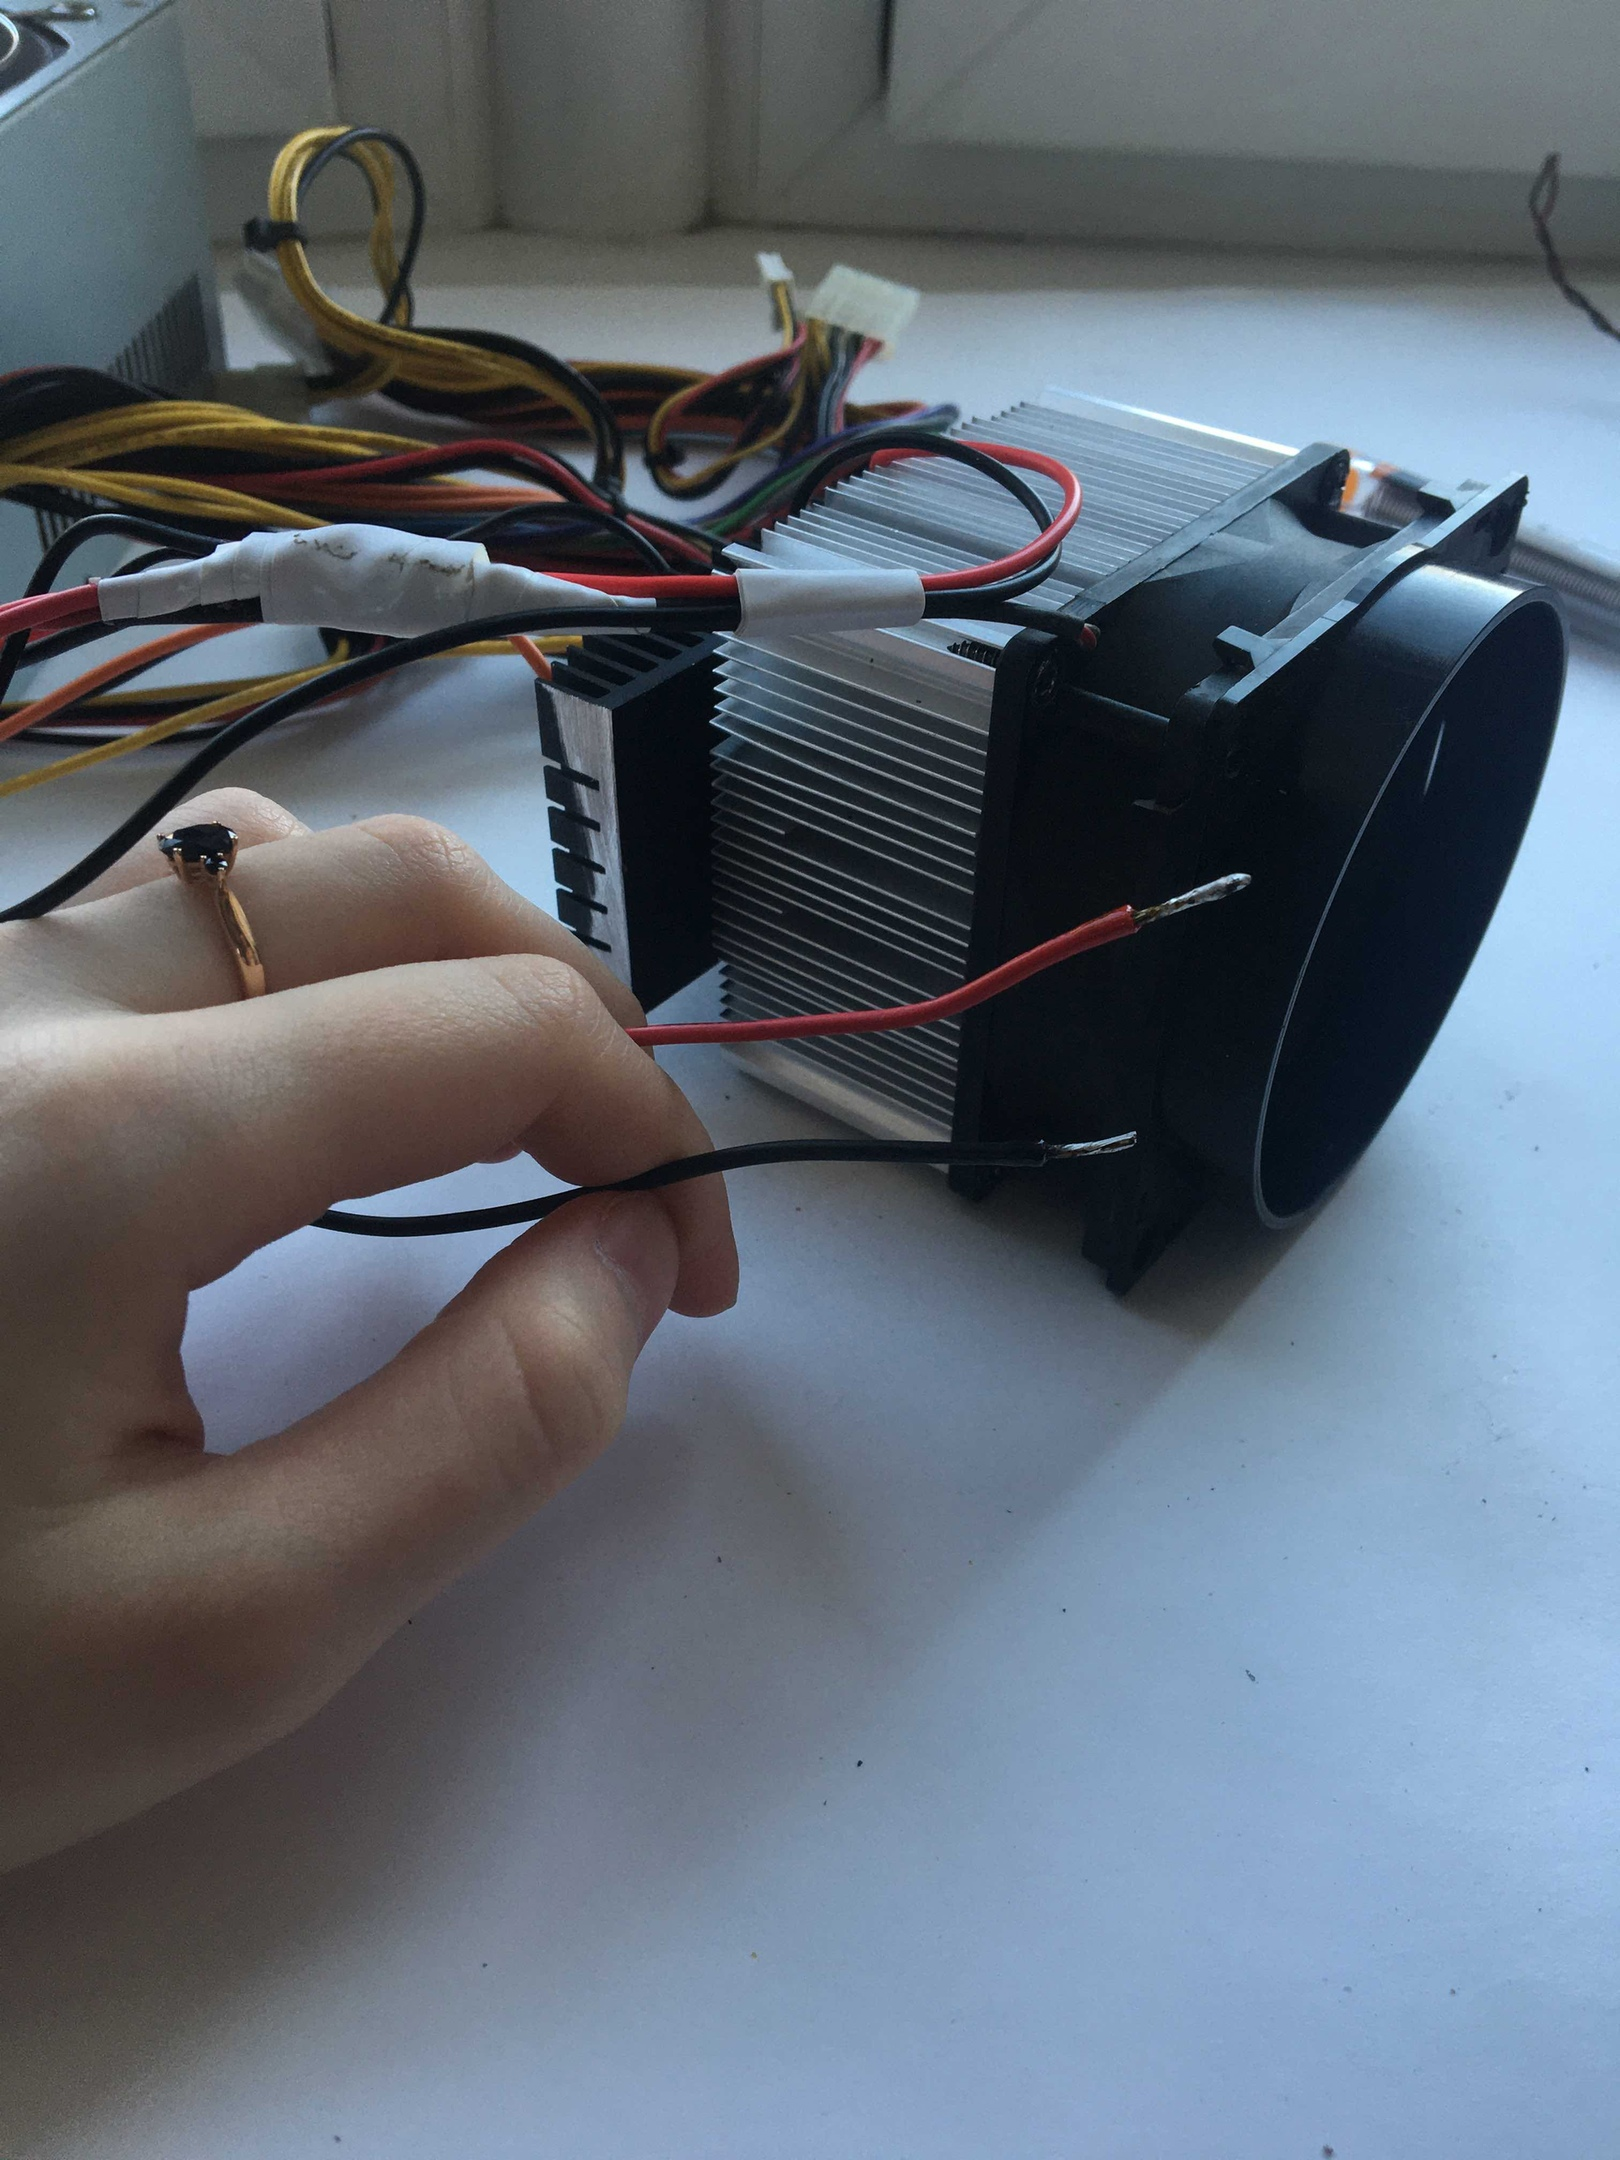
\includegraphics[width = 70mm]{lud.jpg} \\ Лужение}
	\end{minipage}
\end{figure}

\newpage
\begin{figure}[h!]
	\begin{minipage}[h]{0.5\linewidth}
		\center{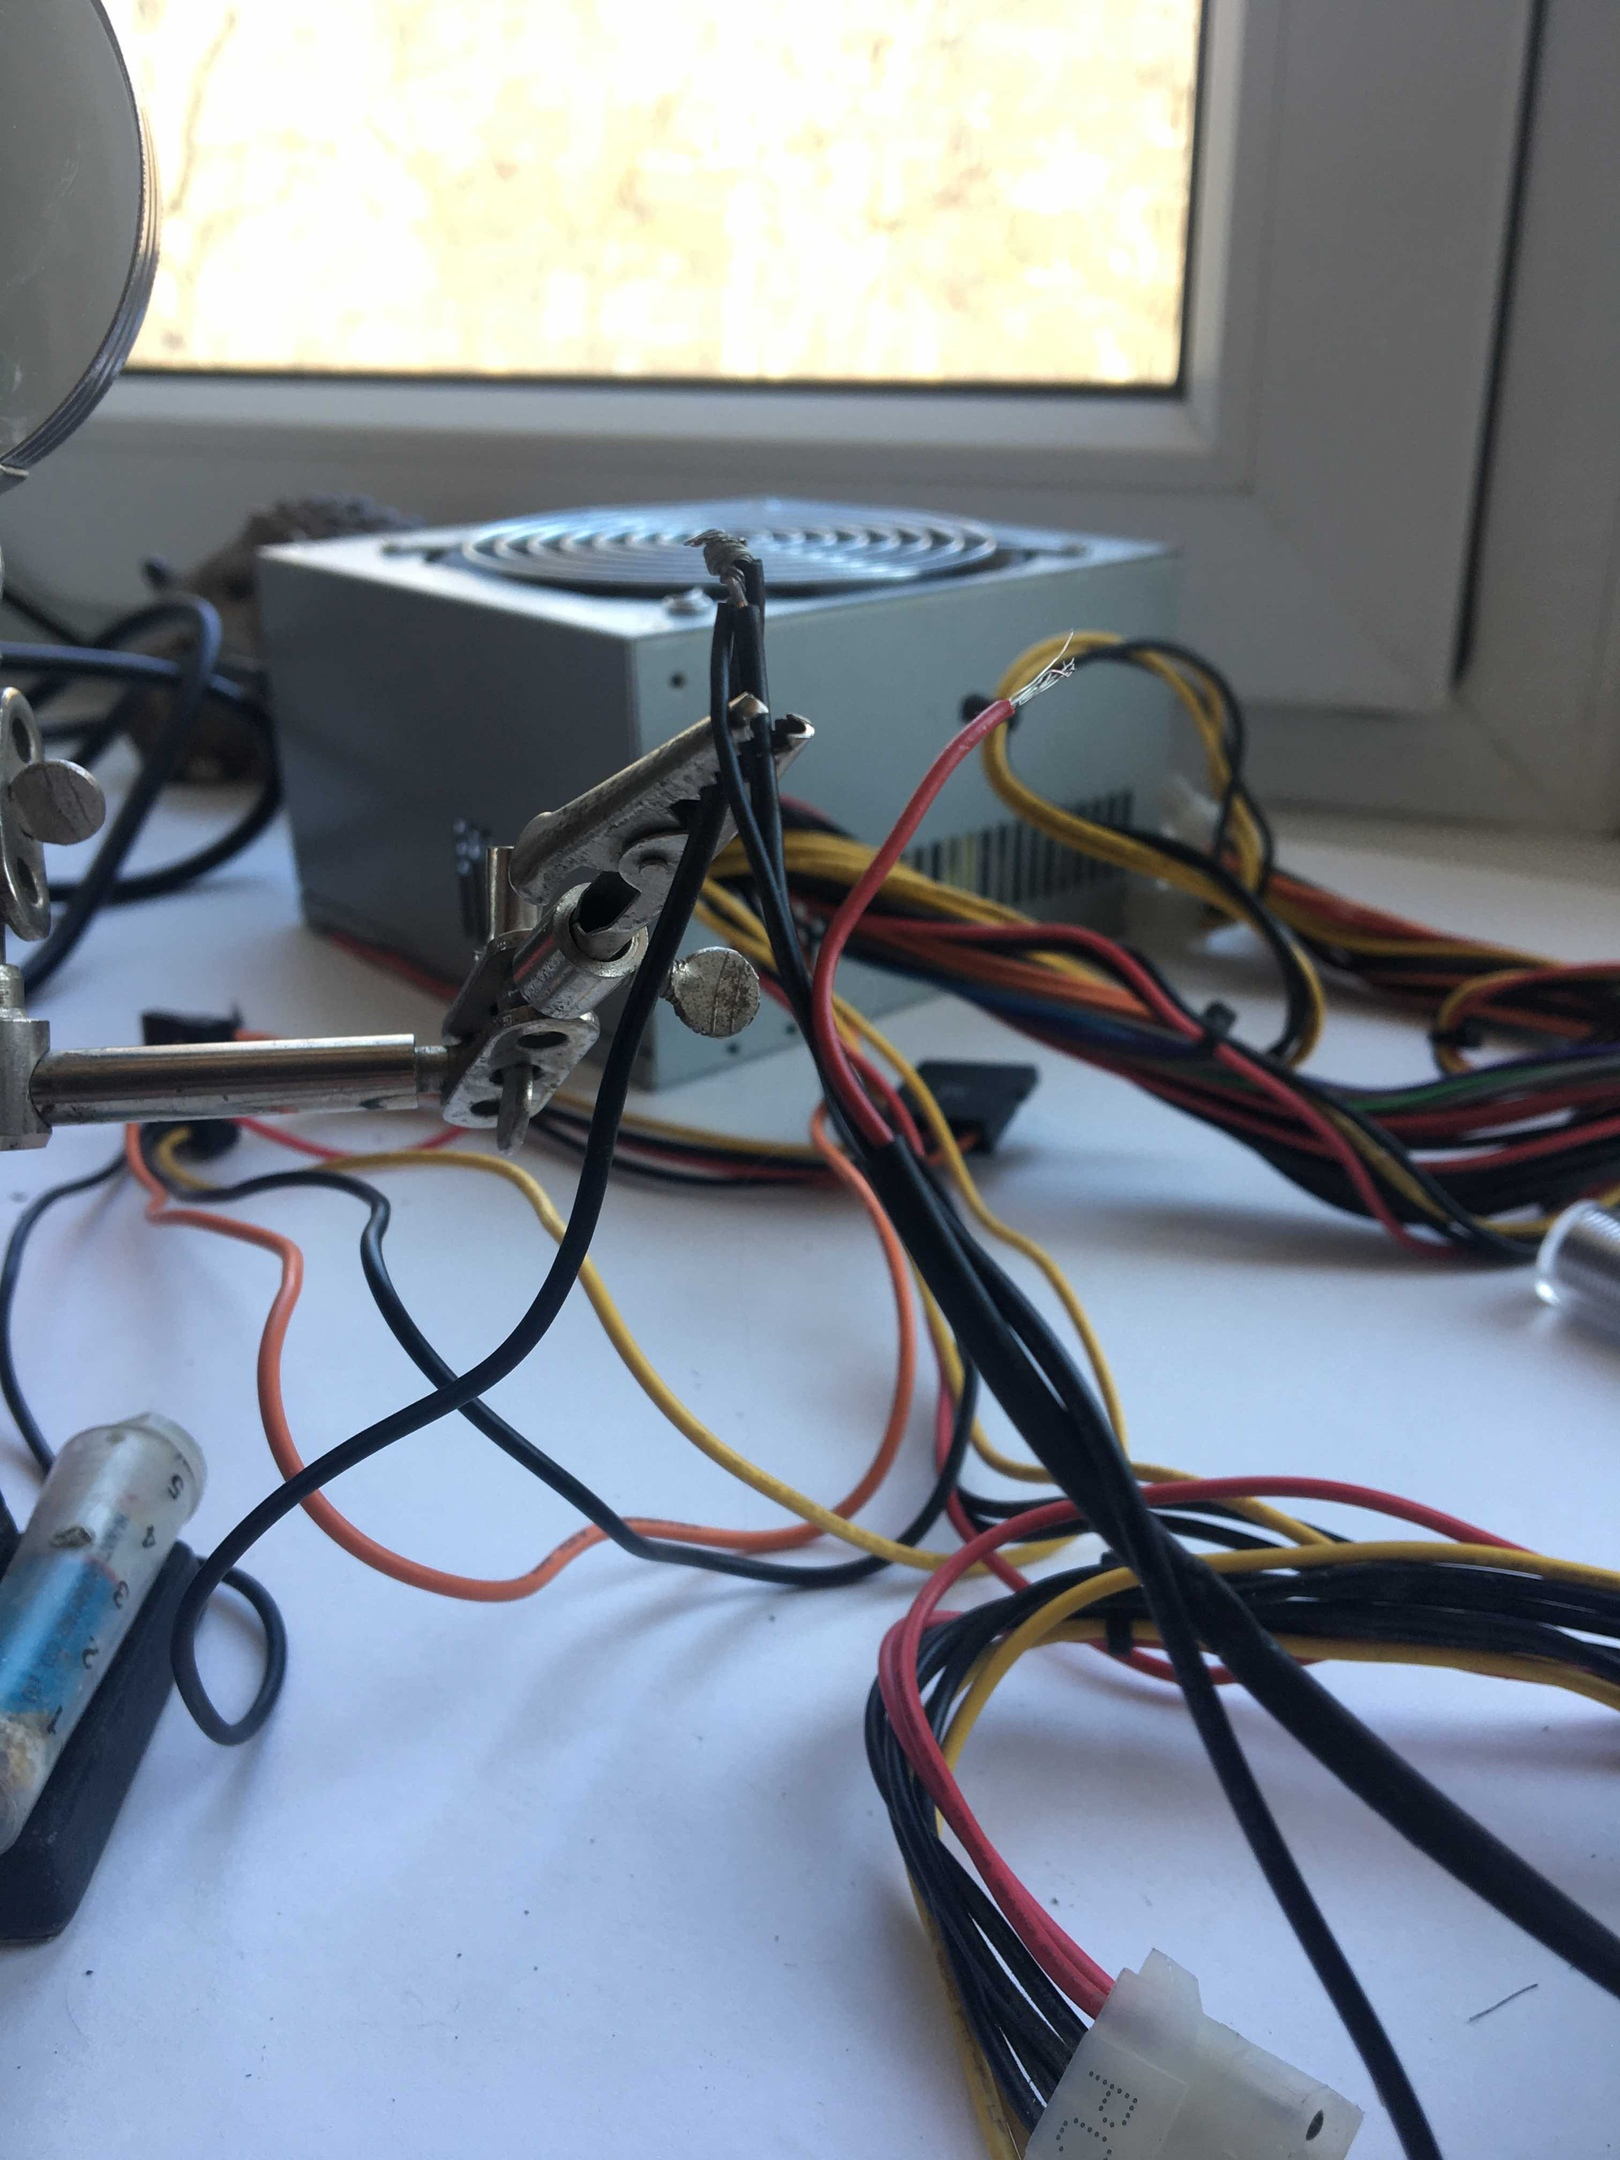
\includegraphics[width = 53mm]{paika1.jpg} \\ Соединение контактов вентилятора и Элемента Пельтье}
	\end{minipage}
	\hfill
	\begin{minipage}[h]{0.5\linewidth}
		\center{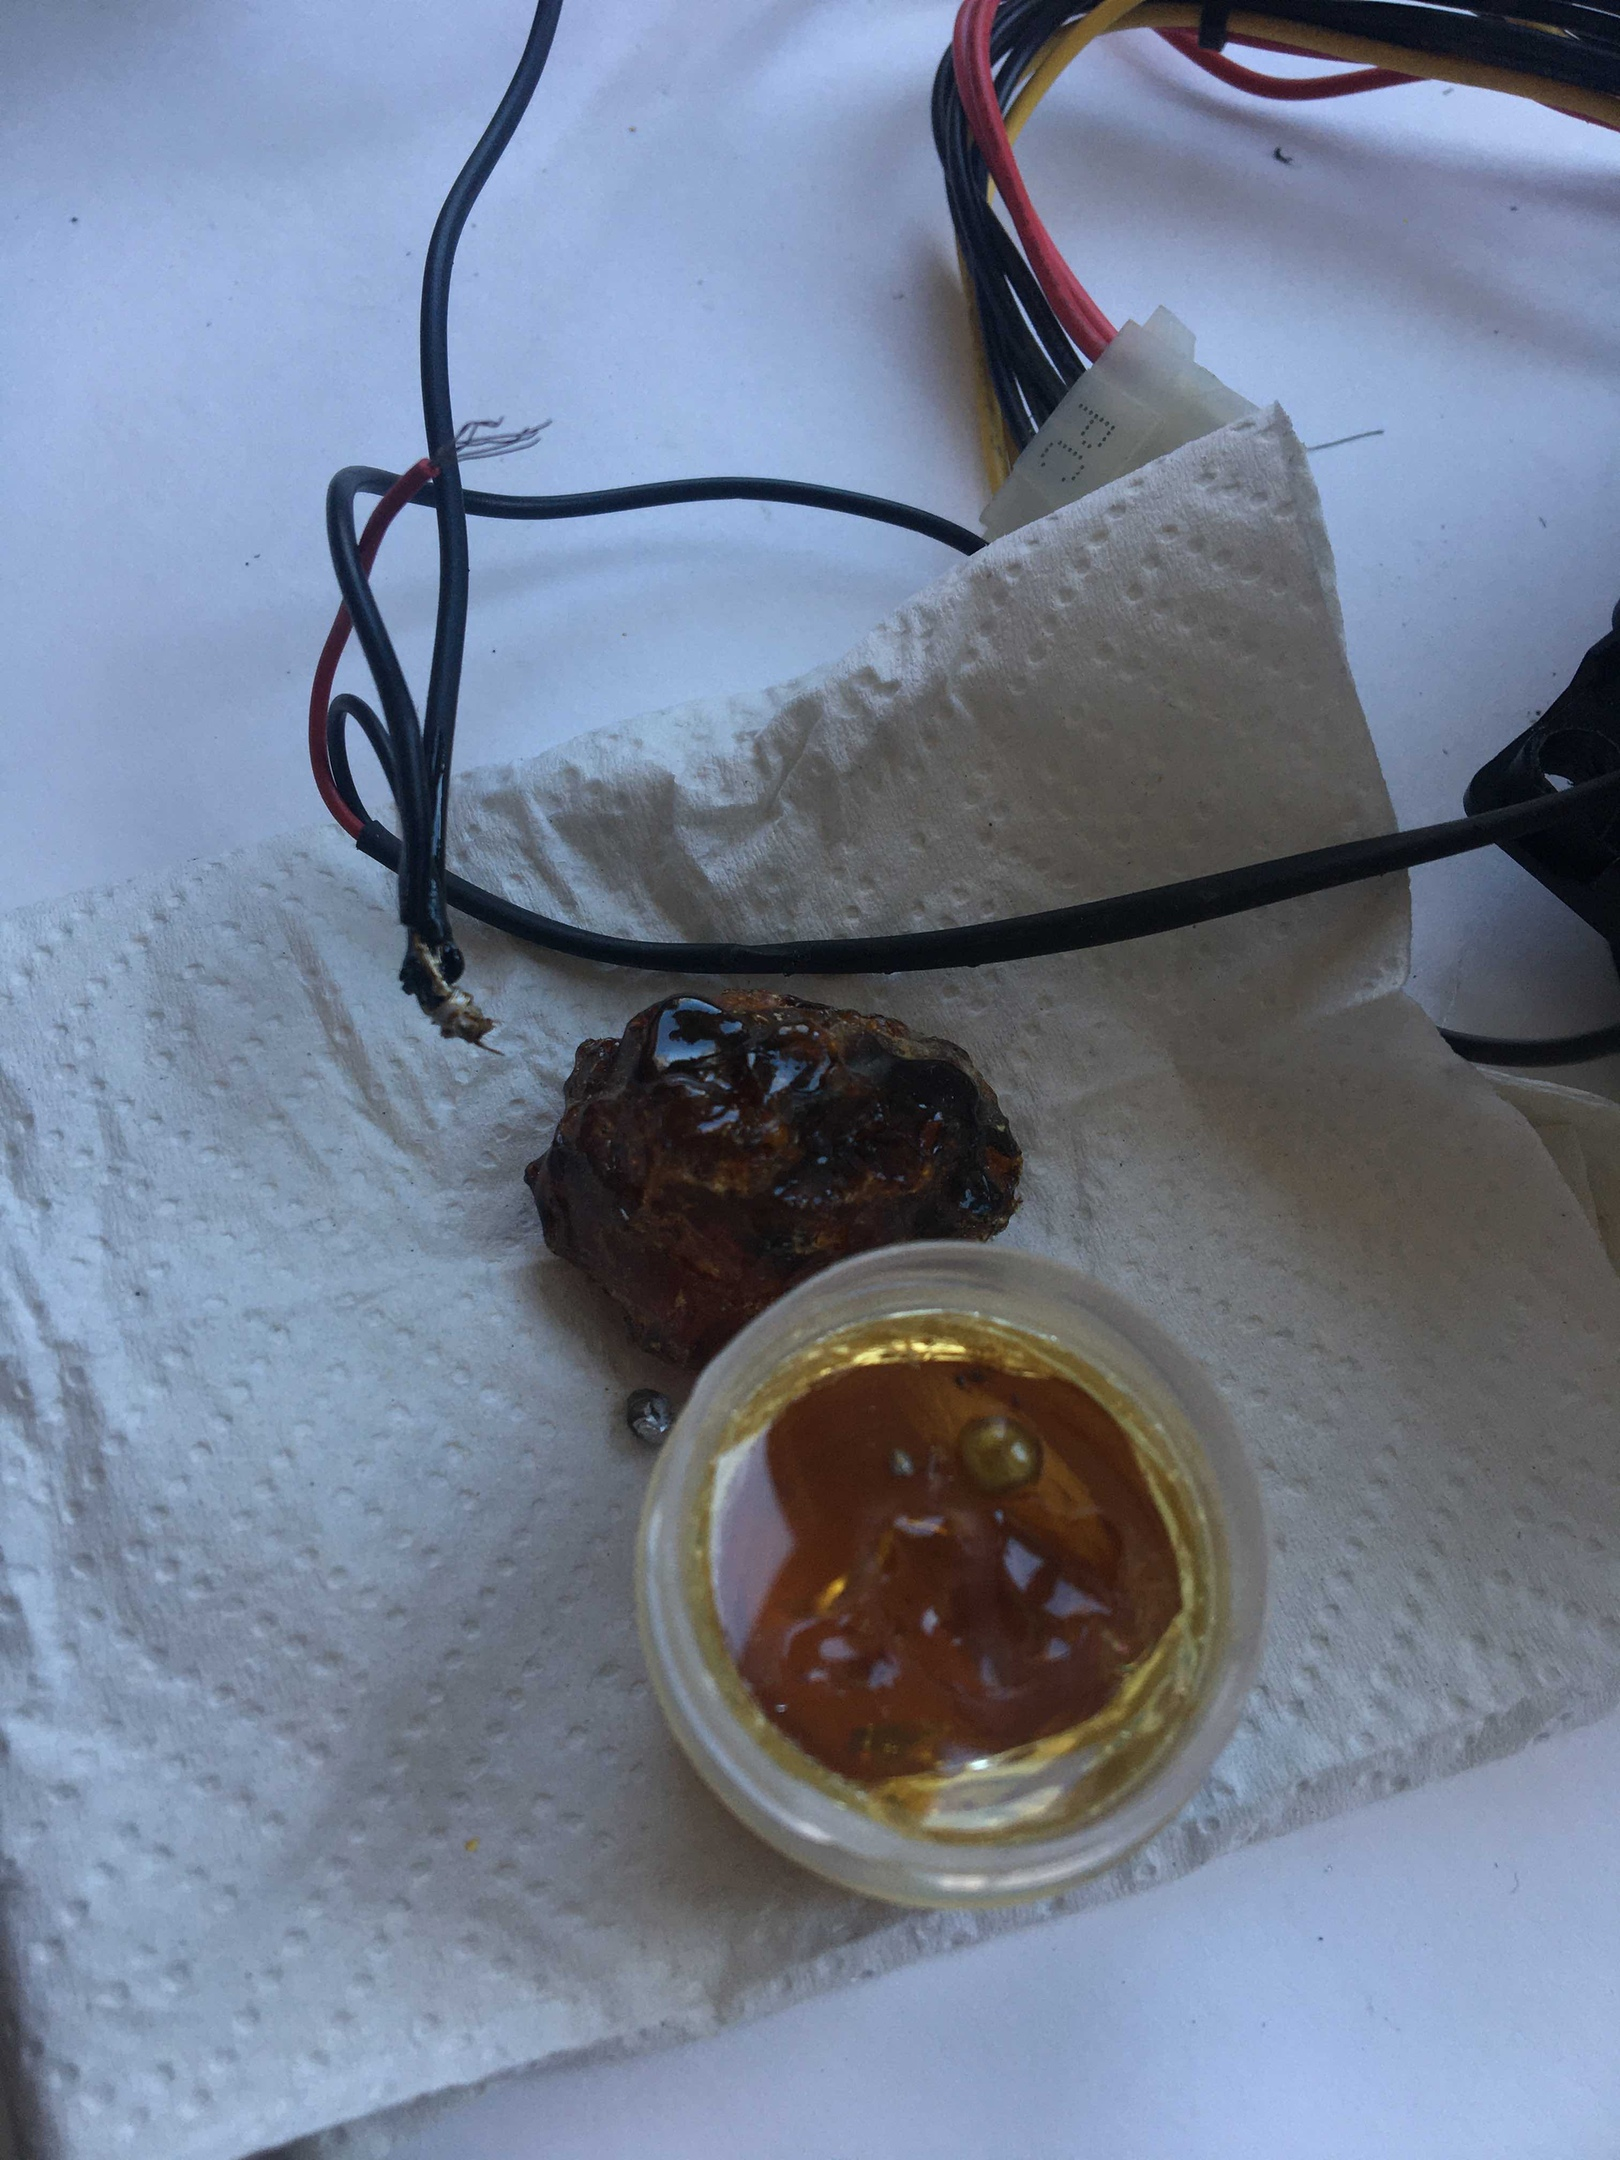
\includegraphics[width = 55mm]{paika2.jpg} \\ Пайка}
	\end{minipage}
\end{figure}

\begin{figure}[h!]
	\begin{minipage}[h]{0.5\linewidth}
		\center{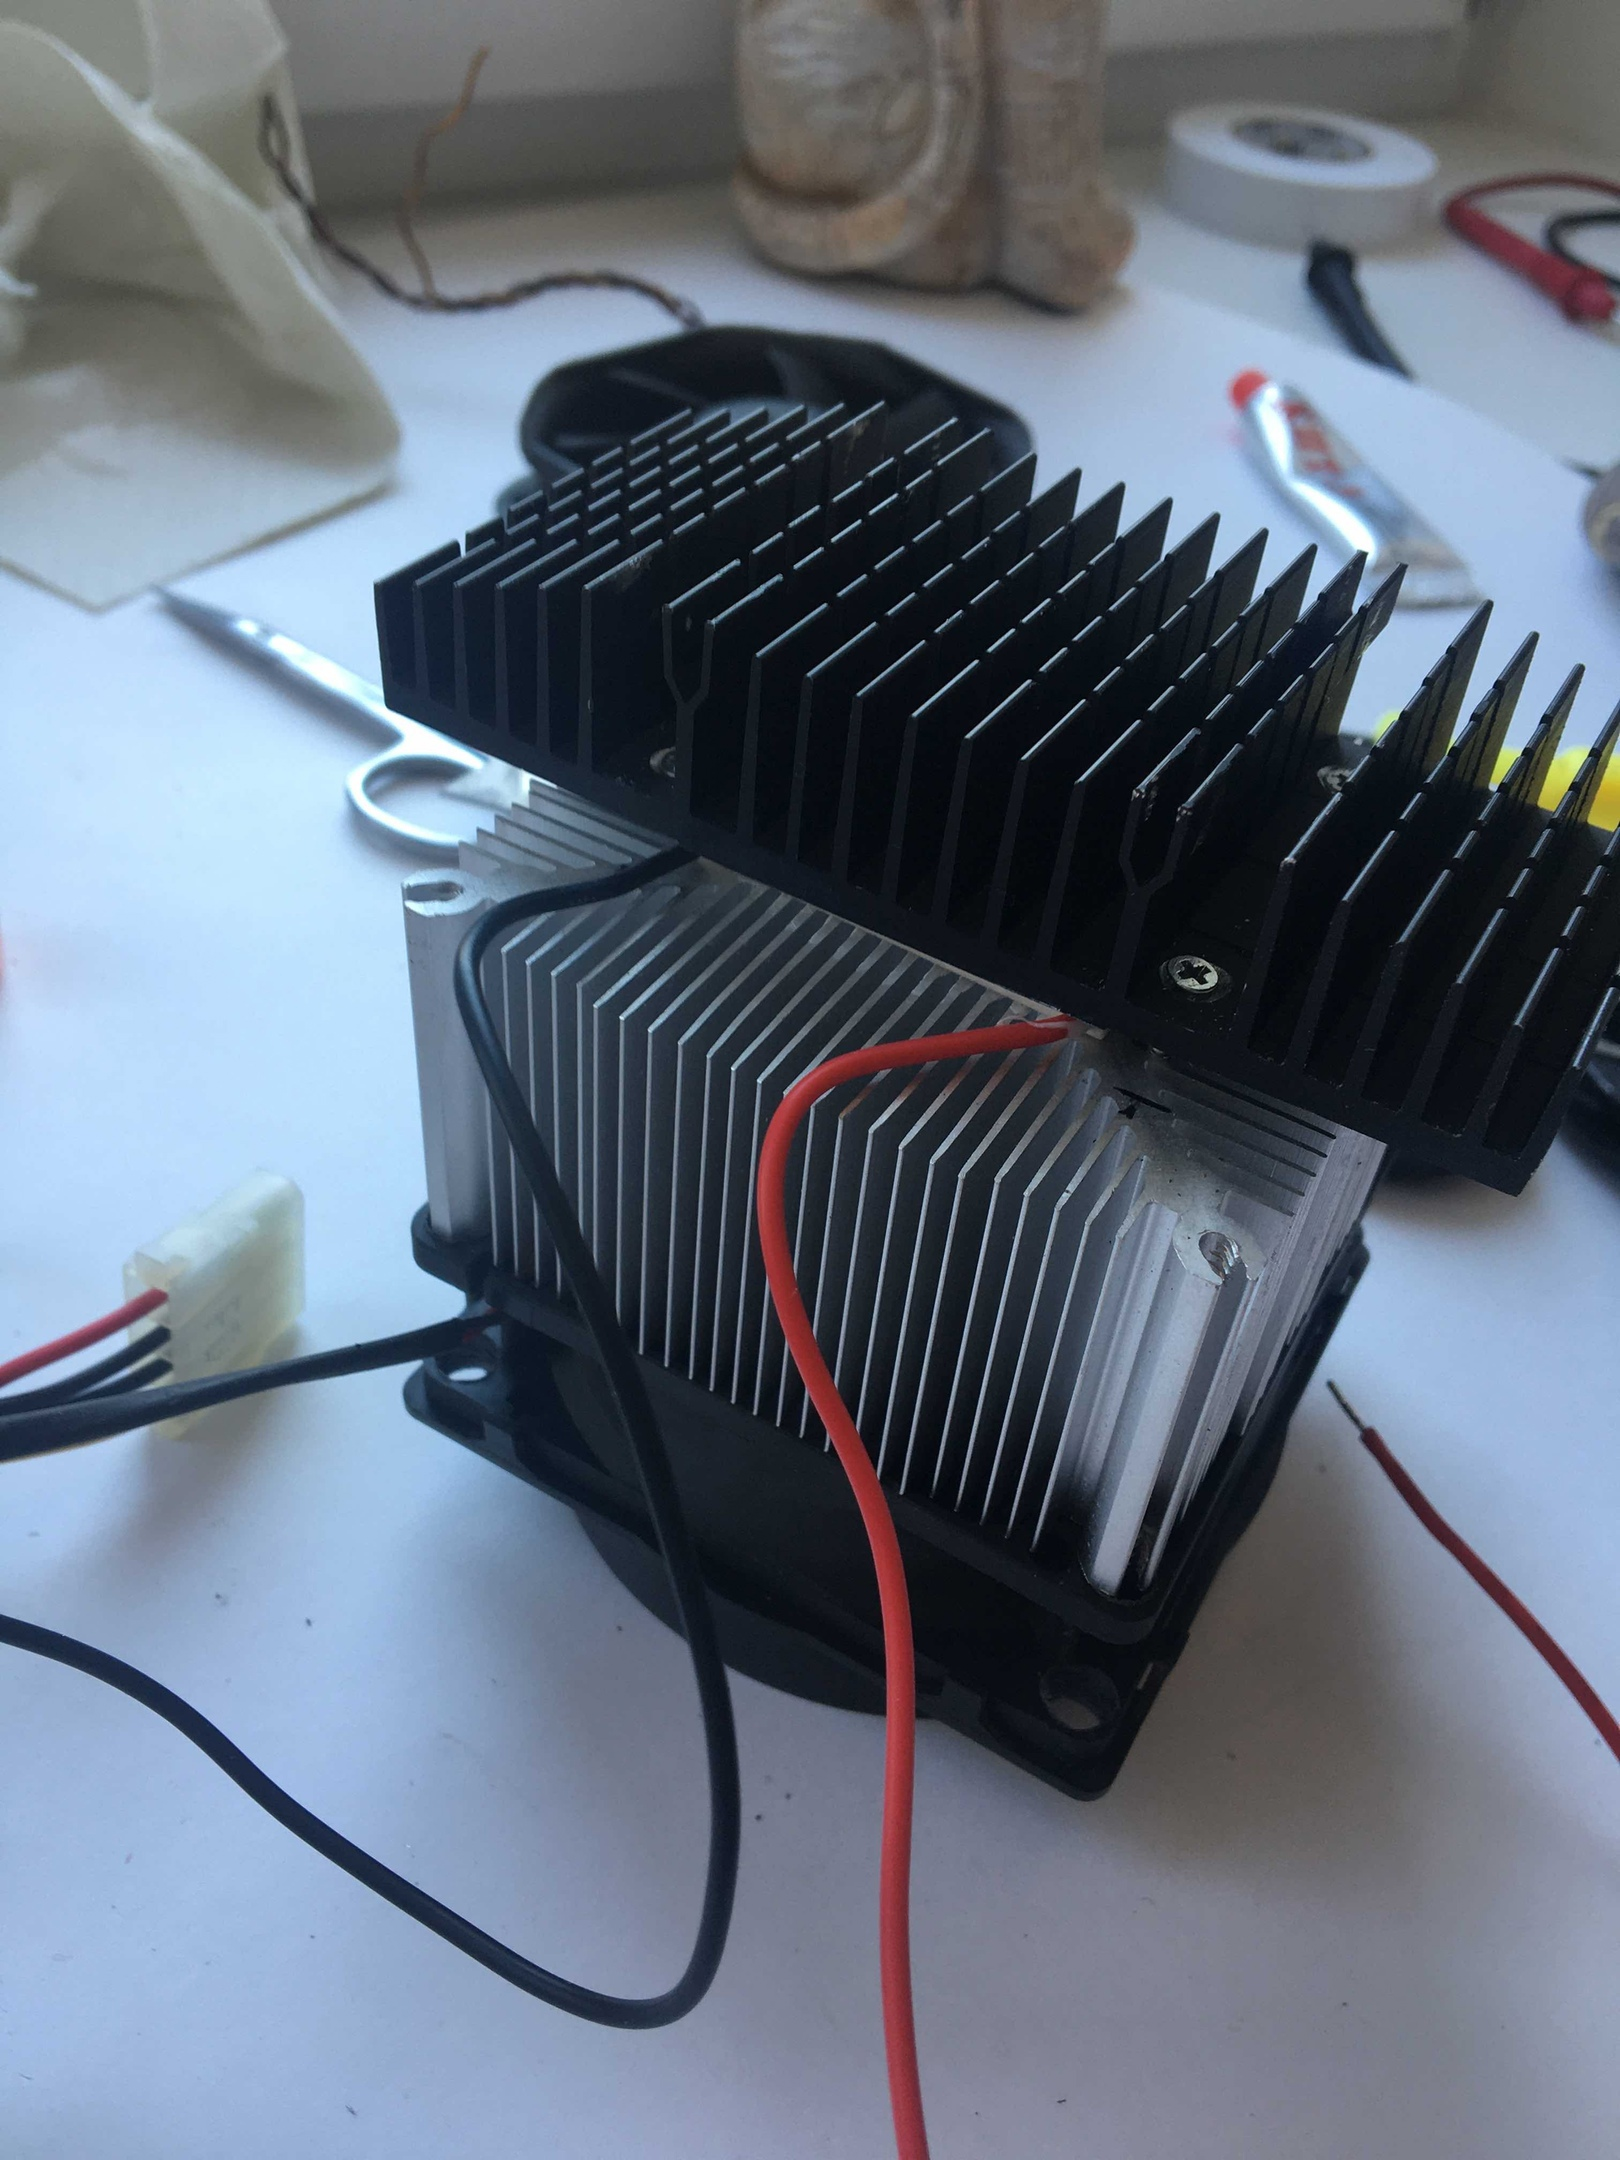
\includegraphics[width = 53mm]{final.jpg} \\ Собранная модель}
	\end{minipage}
	\hfill
	\begin{minipage}[h]{0.5\linewidth}
		\center{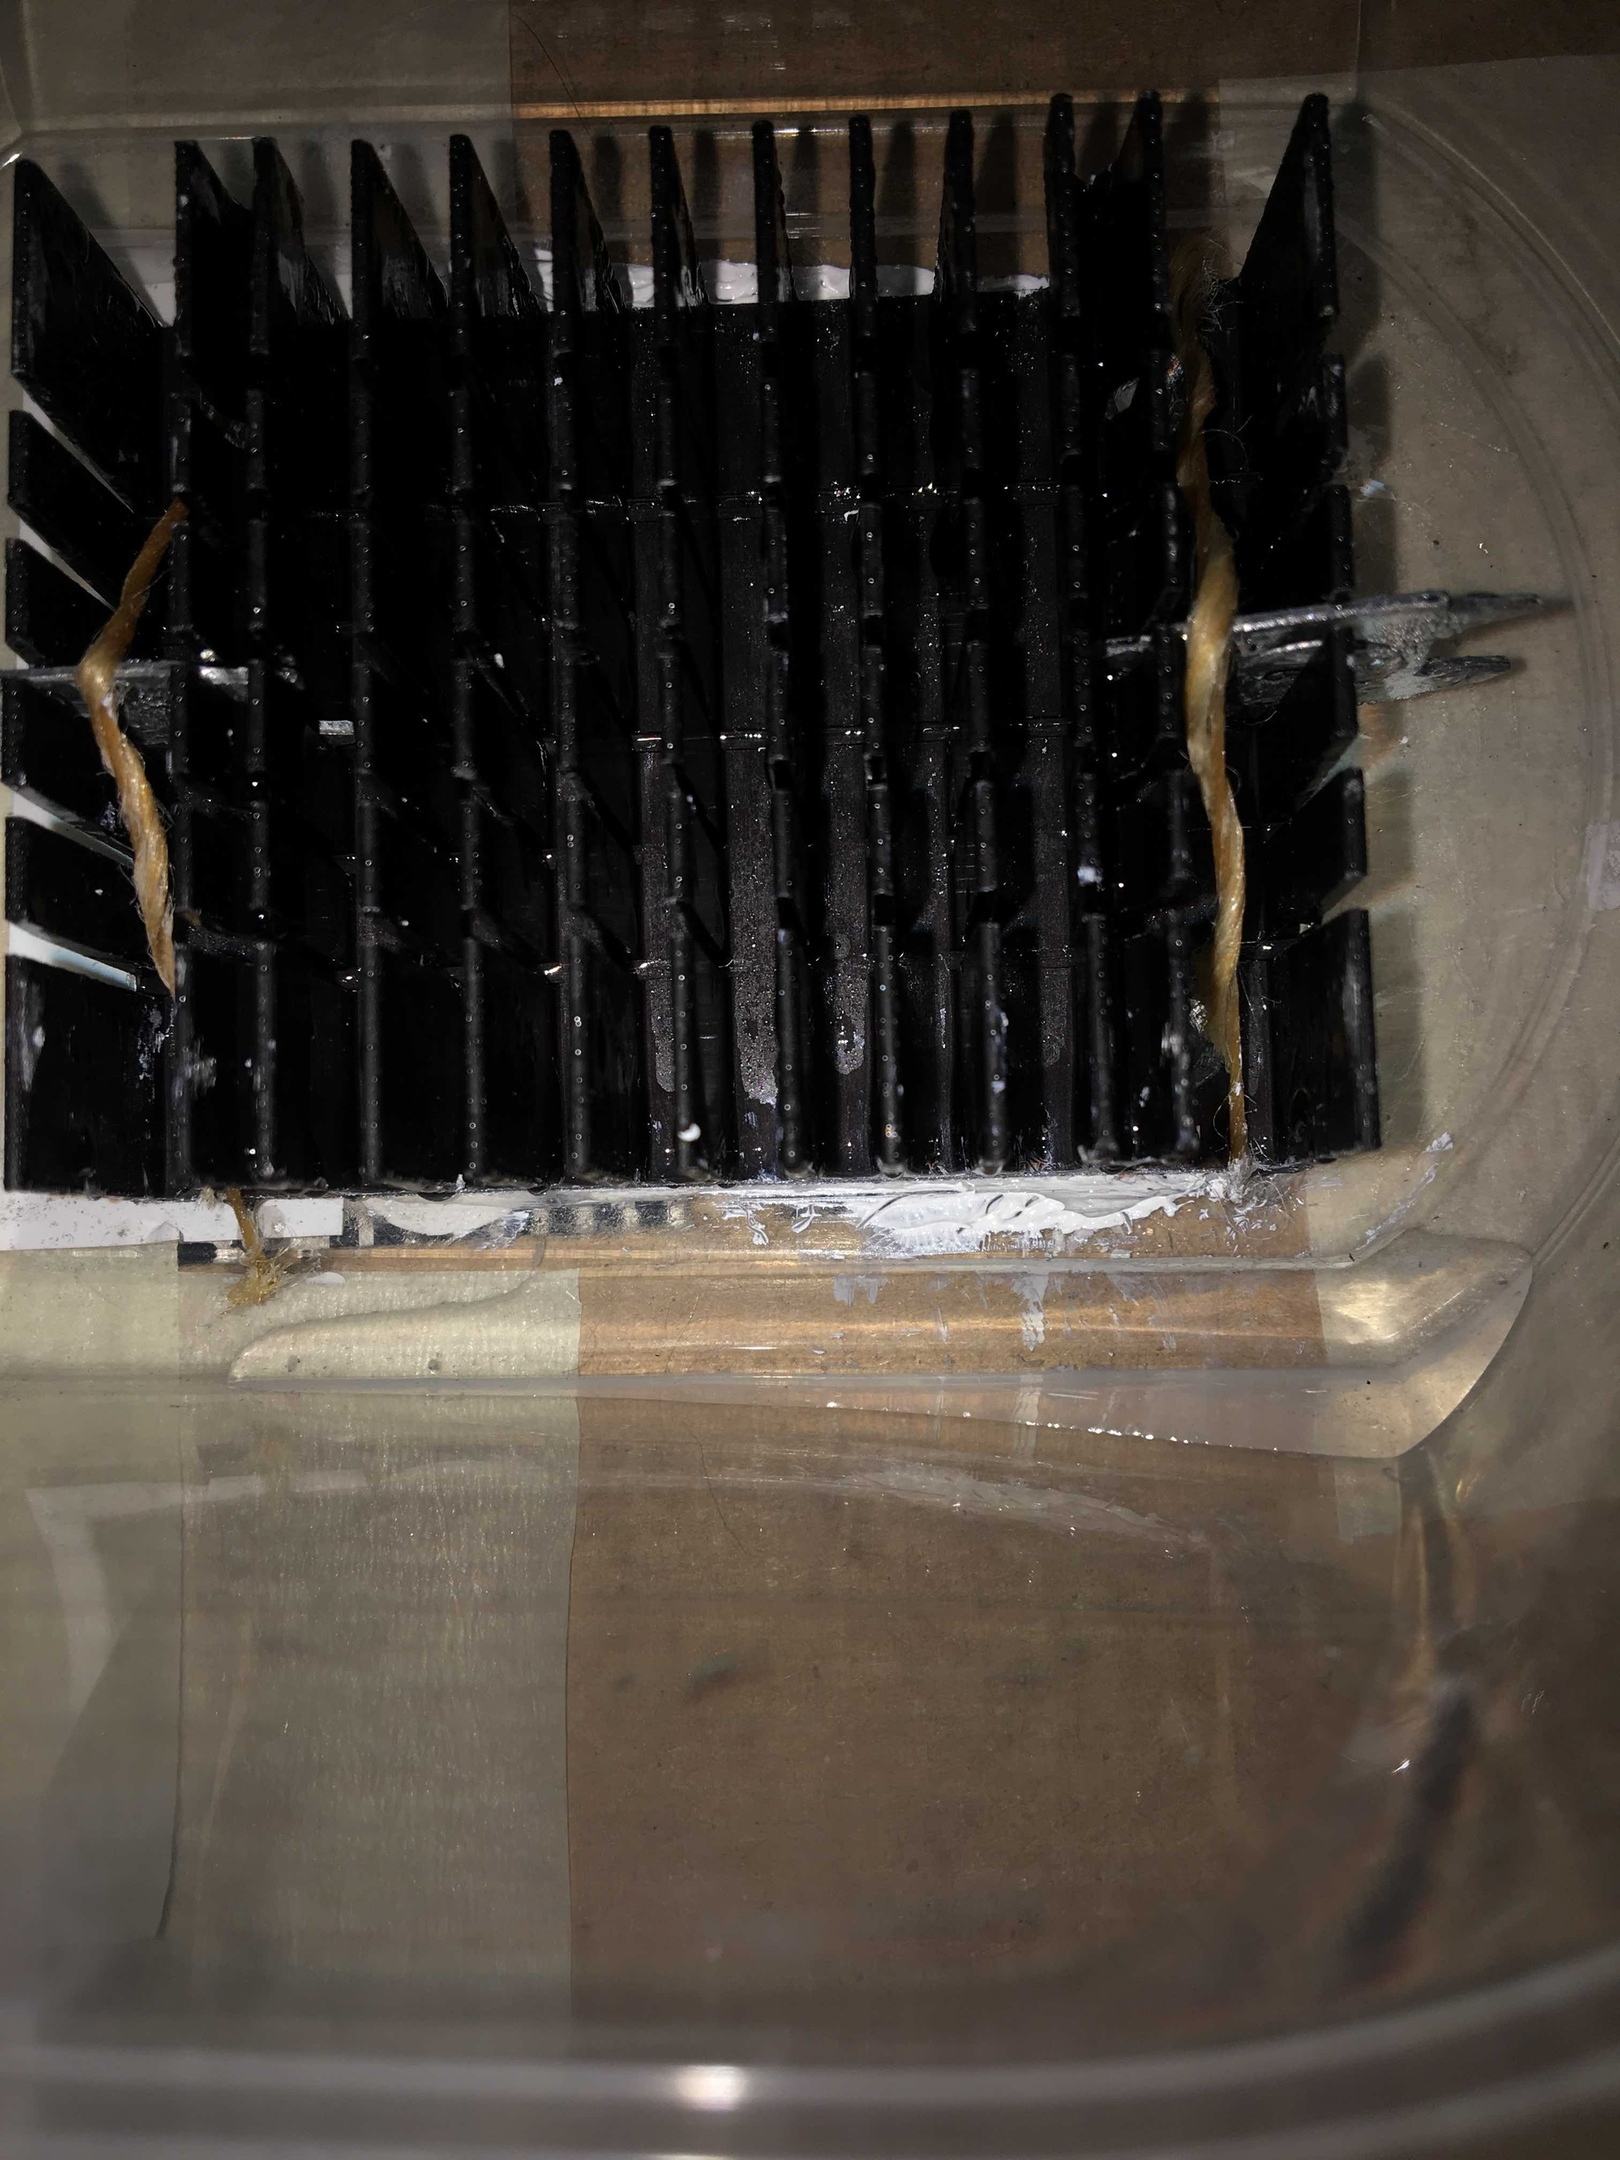
\includegraphics[width = 53mm]{alpha.jpg} \\ Альфа-тестирование}
	\end{minipage}
\end{figure}

\begin{figure}[h!]
	\begin{minipage}[h]{0.5\linewidth}
		\center{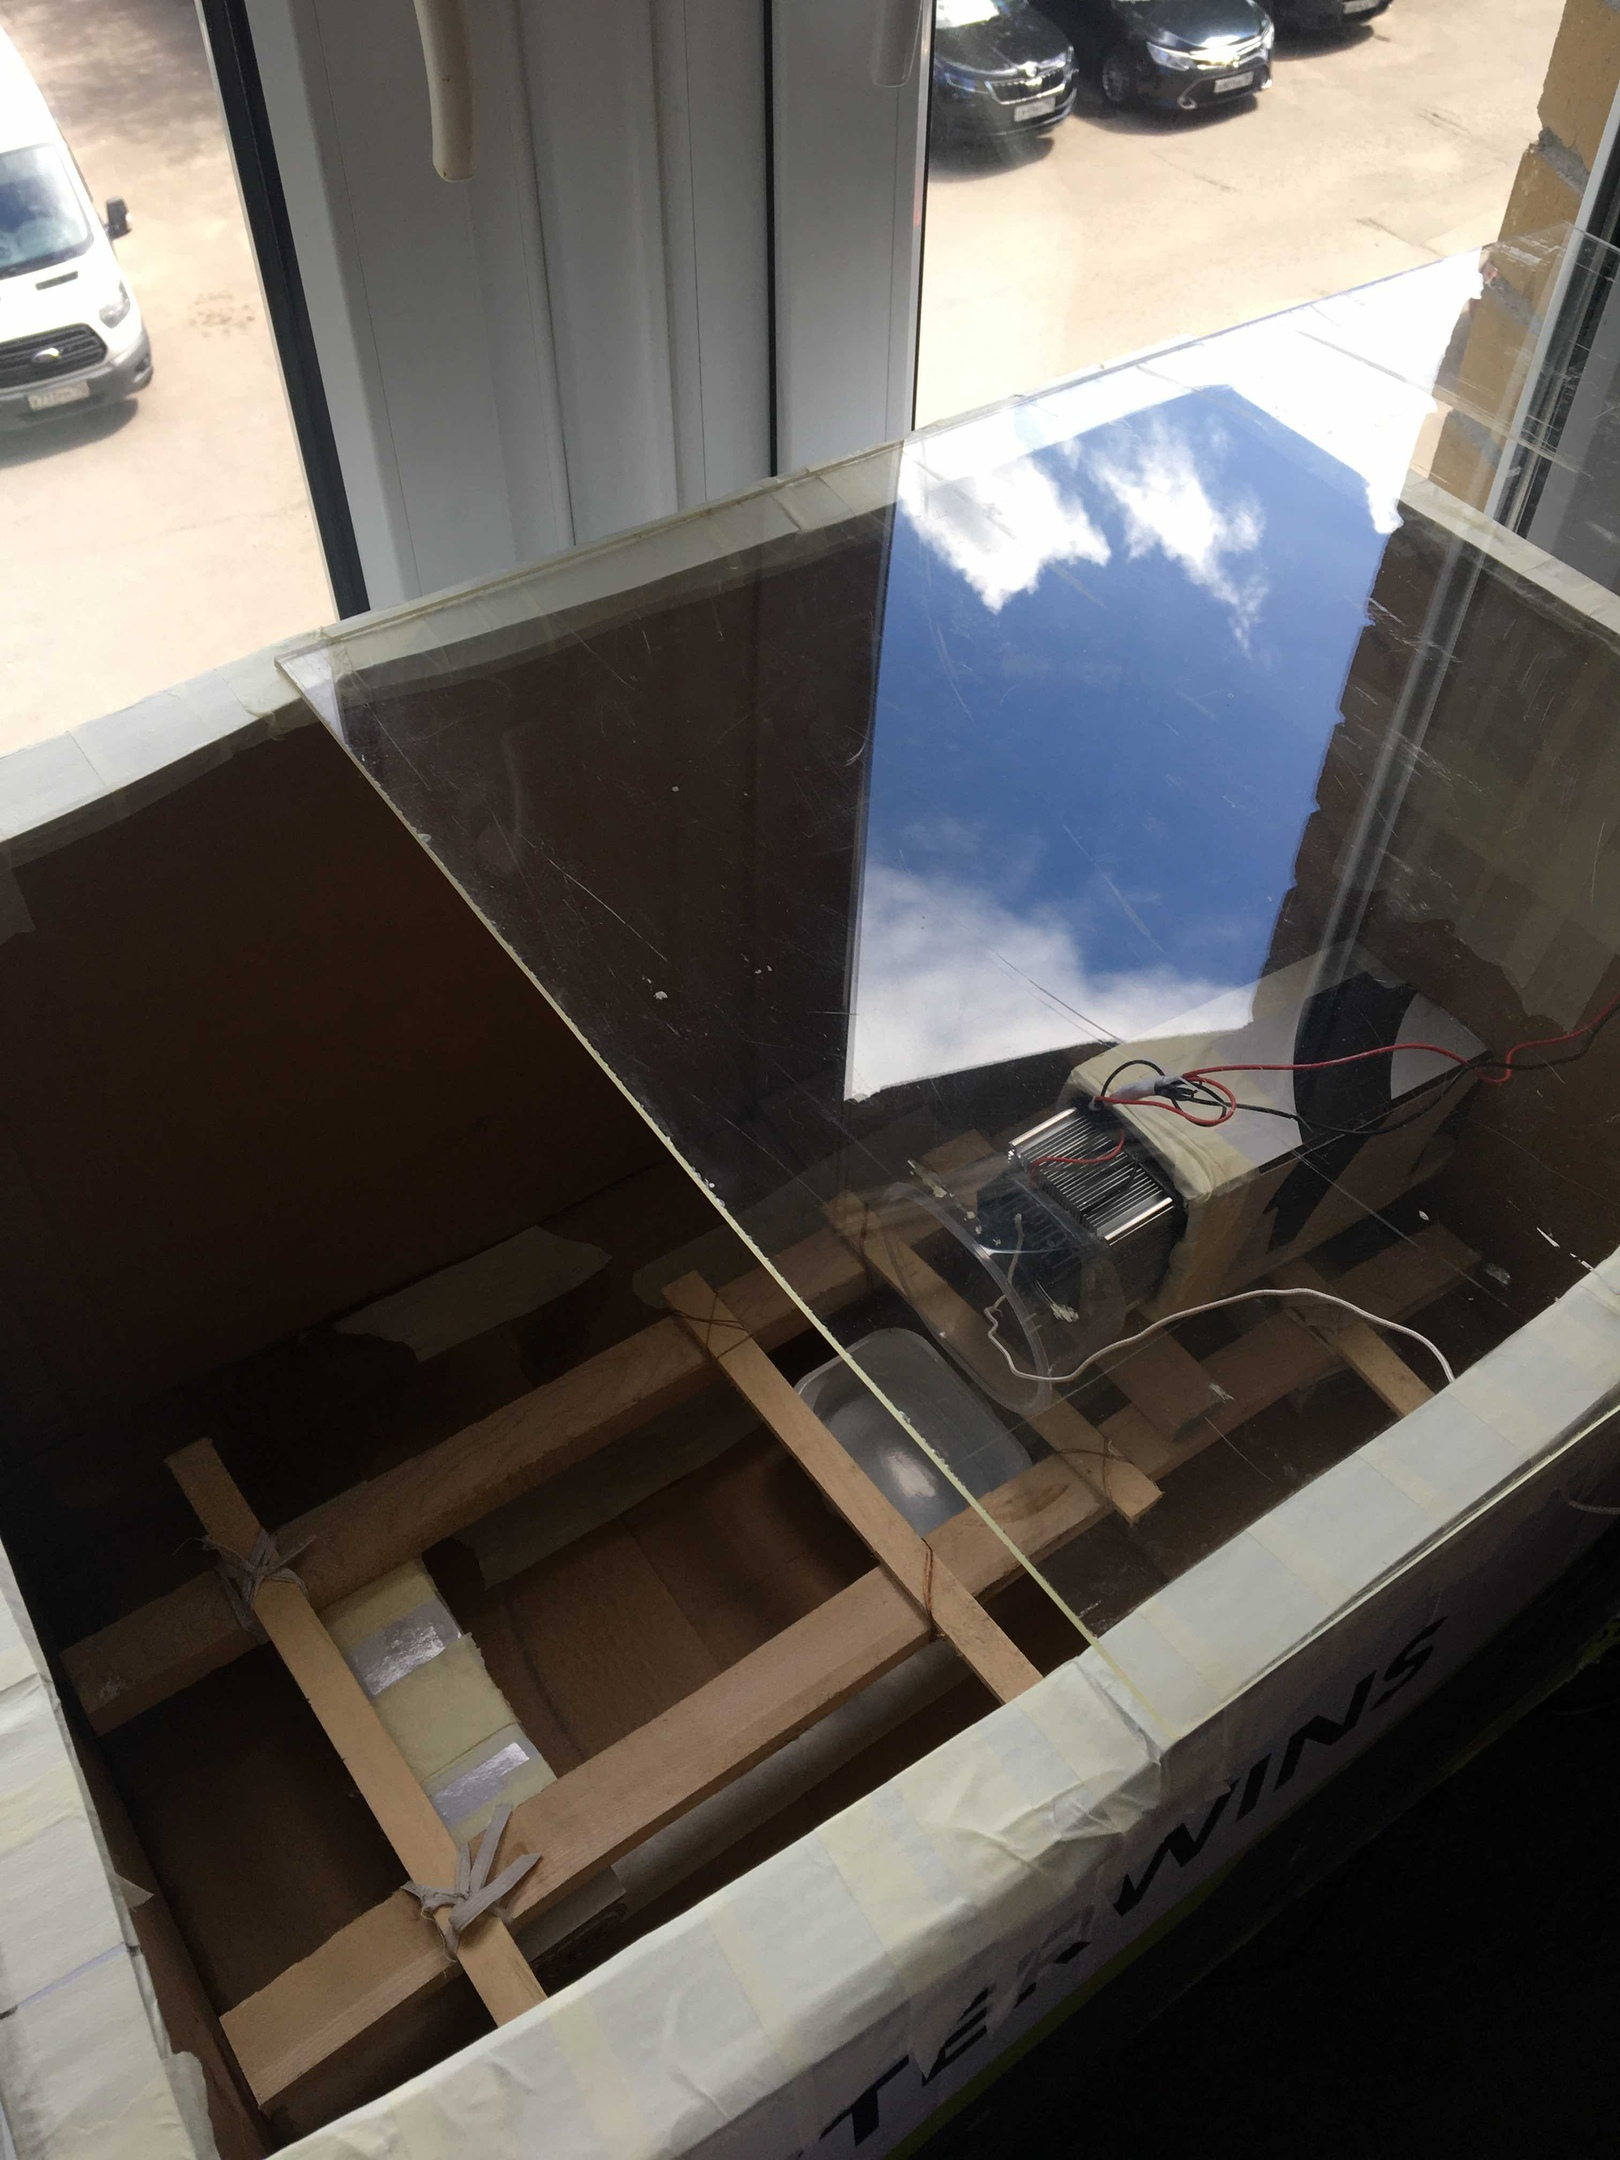
\includegraphics[width = 51mm]{nebo.jpg} \\ Сборка помещения}
	\end{minipage}
	\hfill
	\begin{minipage}[h]{0.5\linewidth}
		\center{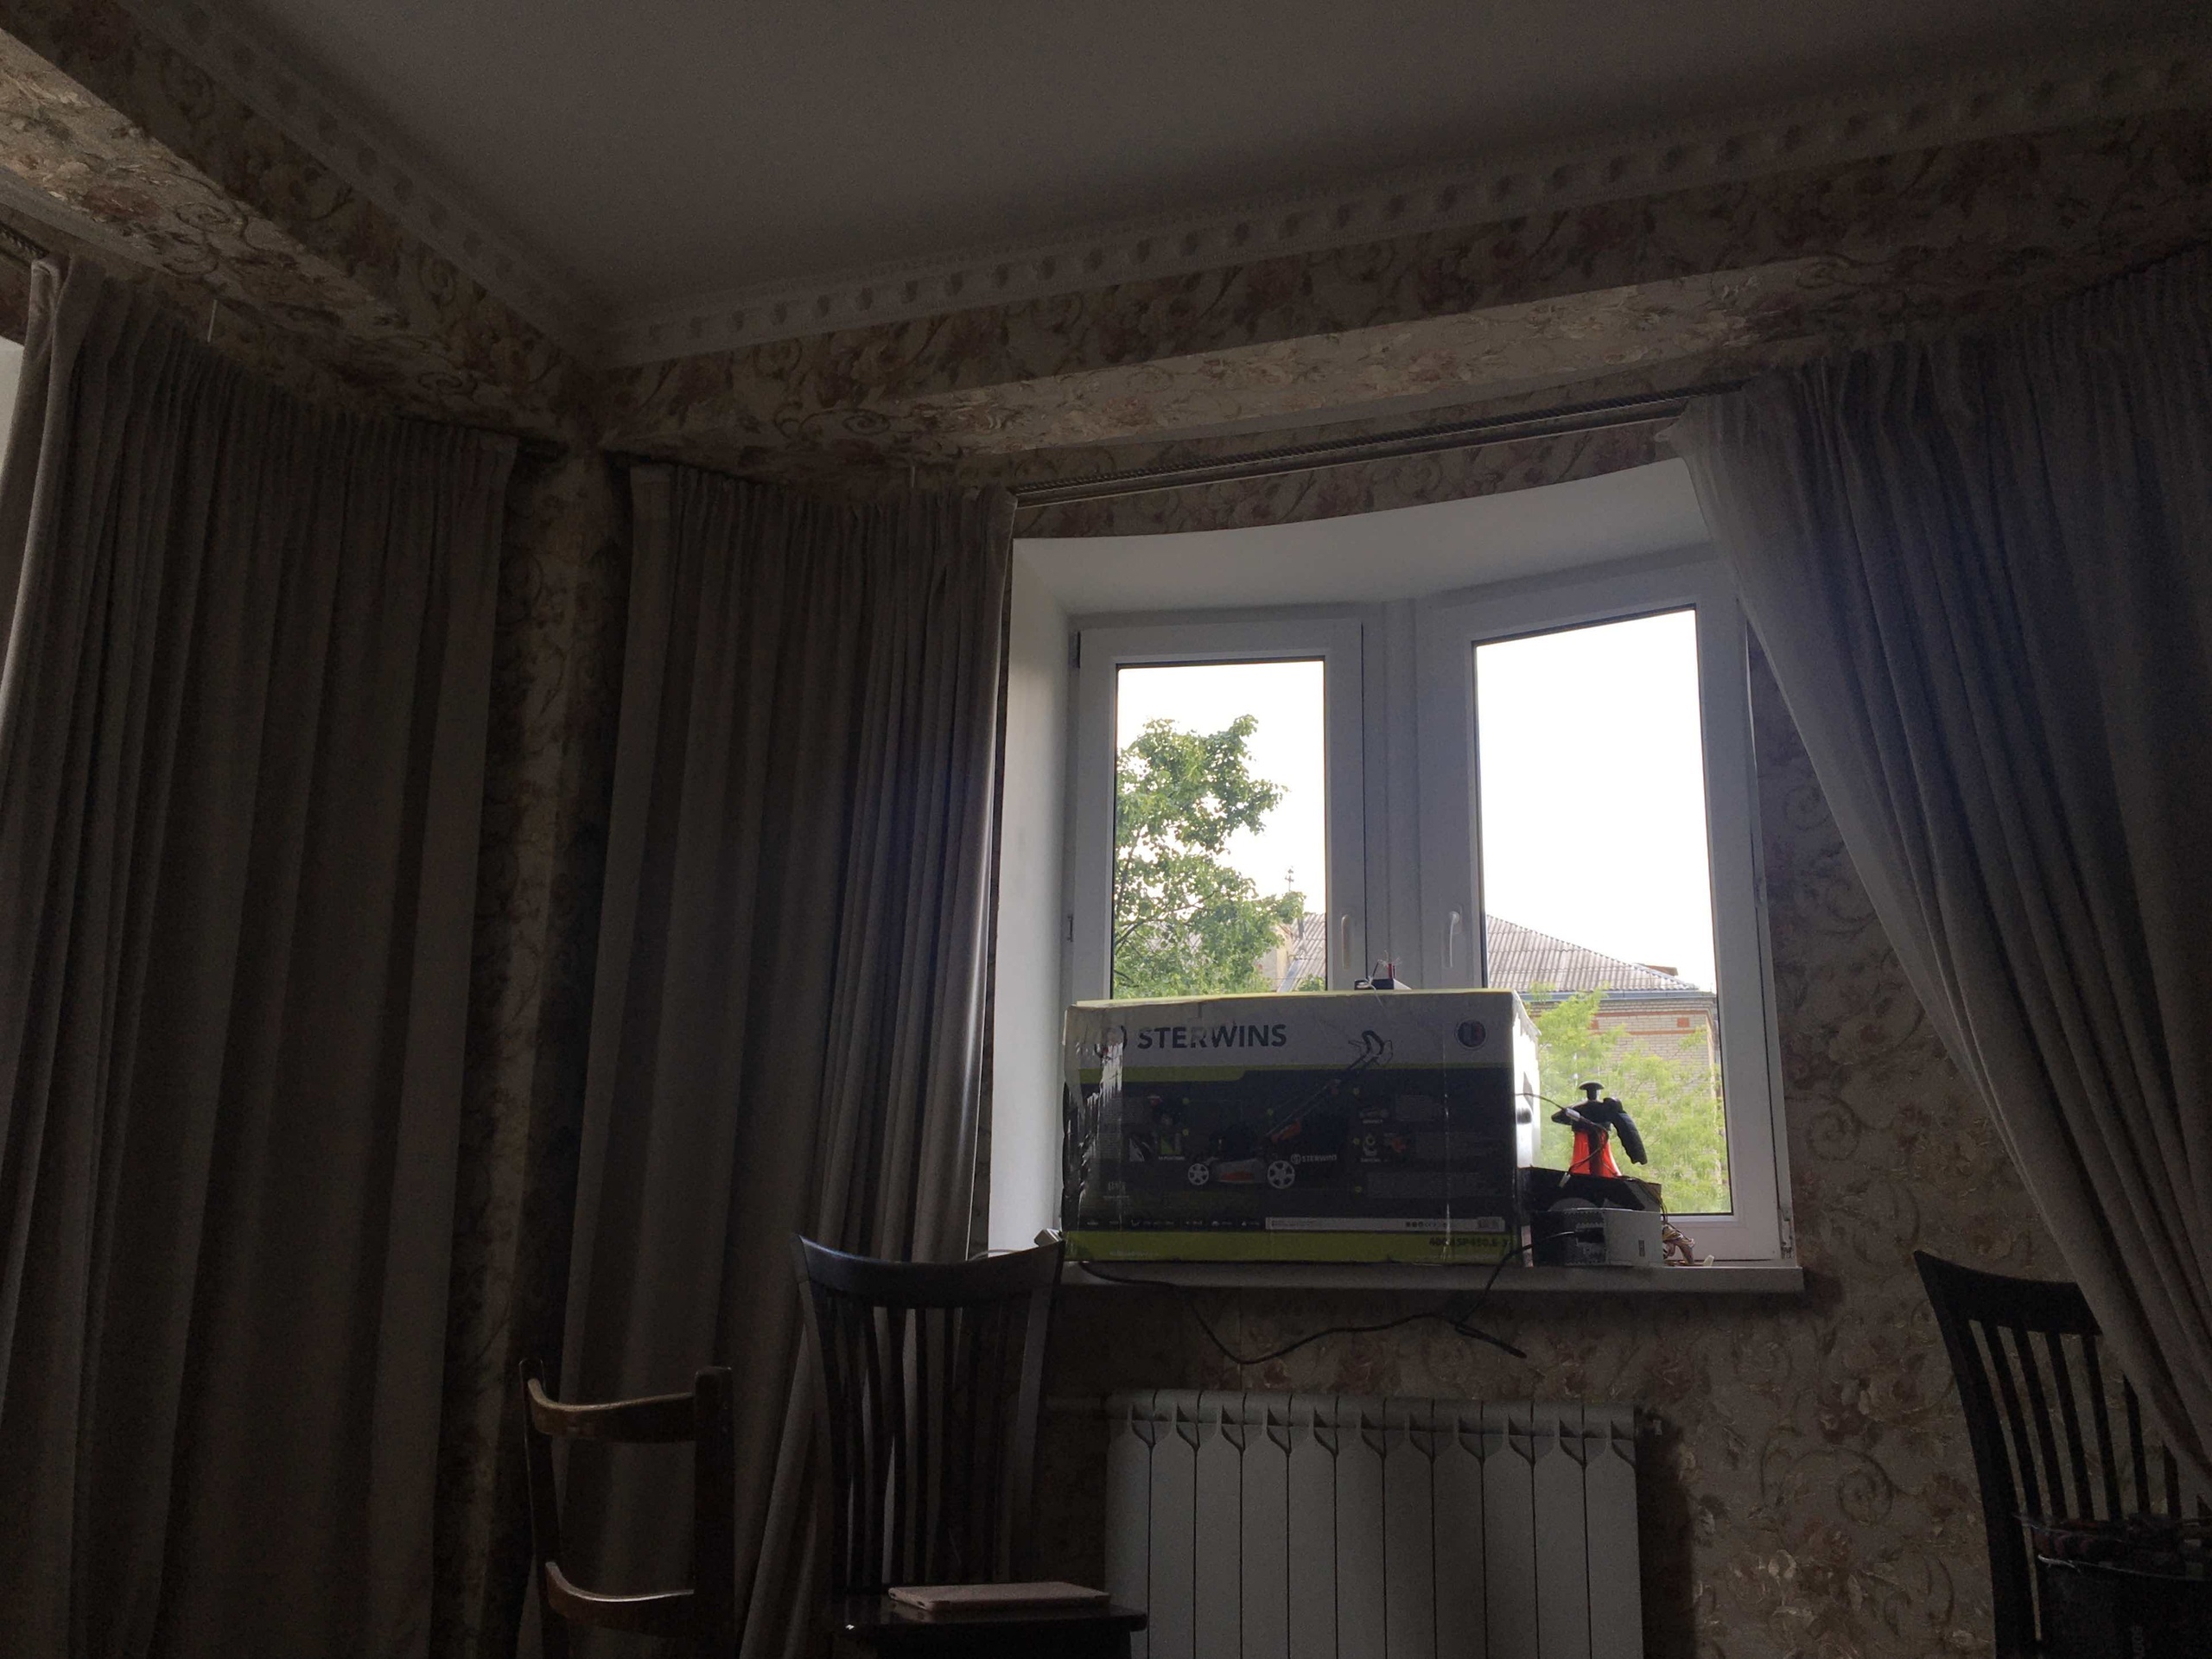
\includegraphics[width = 85mm]{window.jpg} \\ Помещение на окне}
	\end{minipage}
\end{figure}

\newpage
\begin{figure}[h!]
	\begin{minipage}[h]{0.5\linewidth}
		\center{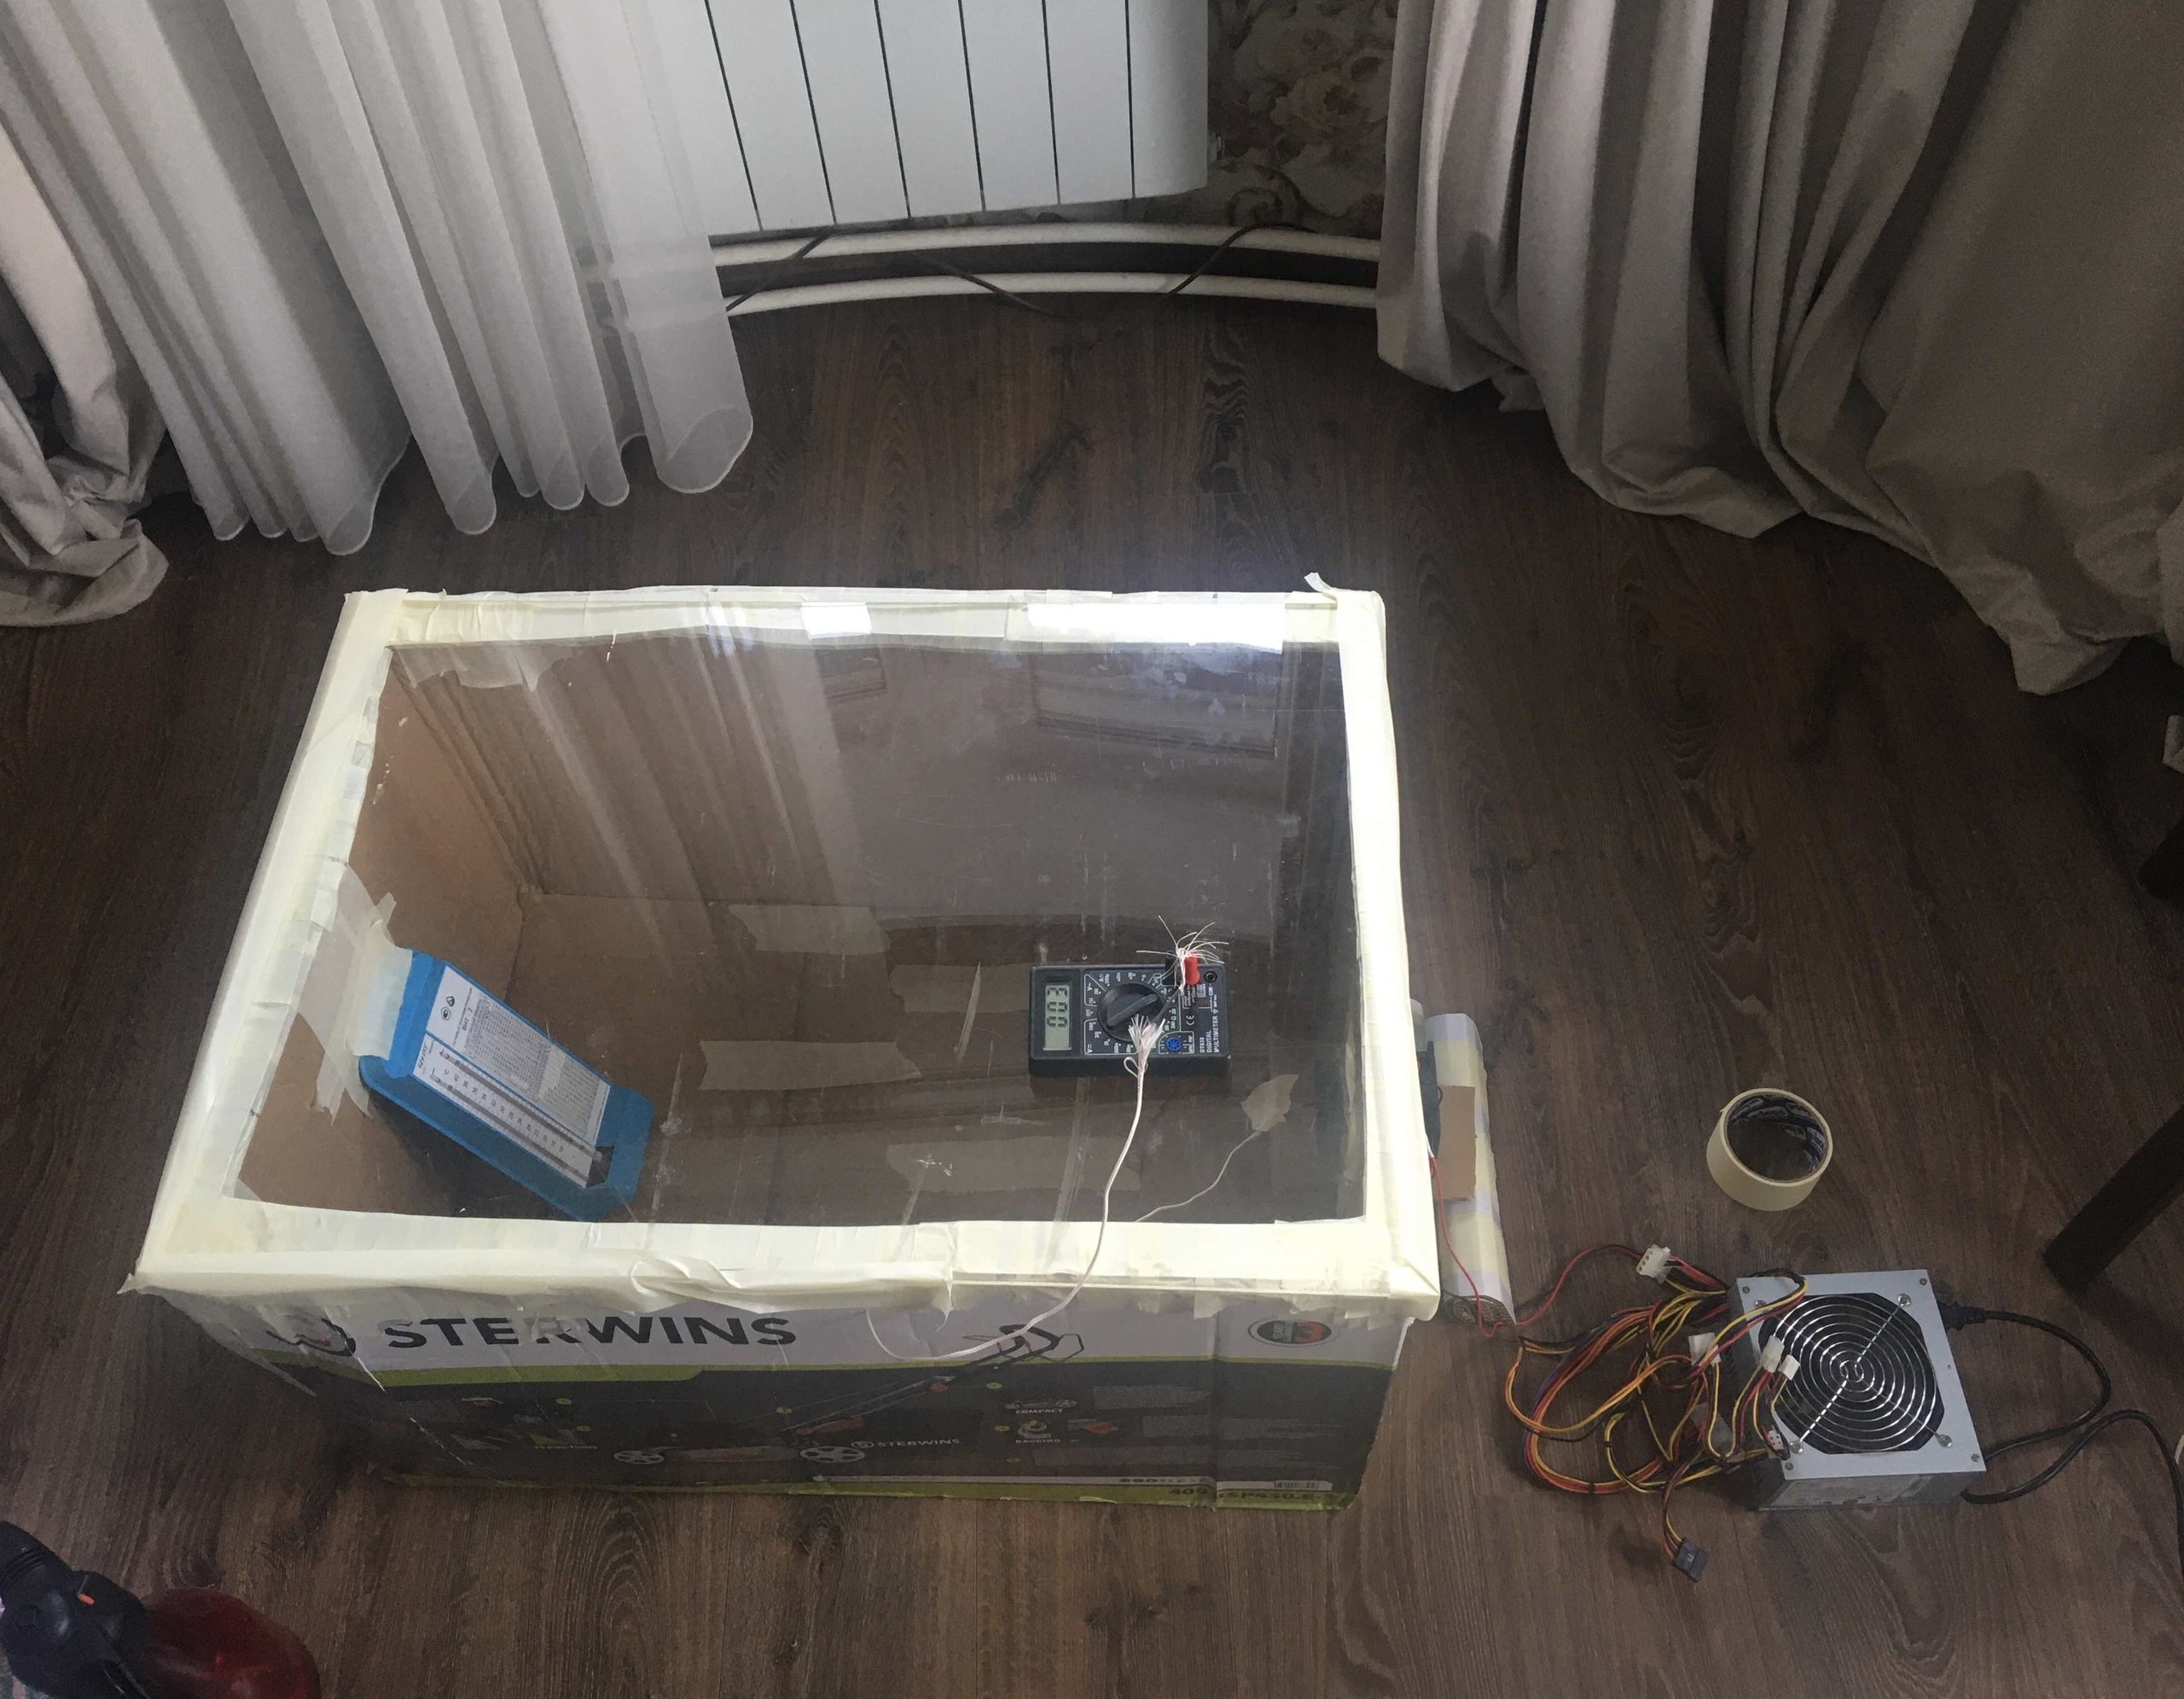
\includegraphics[width = 85mm]{pol1.jpg} \\ Помещение на полу}
	\end{minipage}
	\hfill
	\begin{minipage}[h]{0.5\linewidth}
		\center{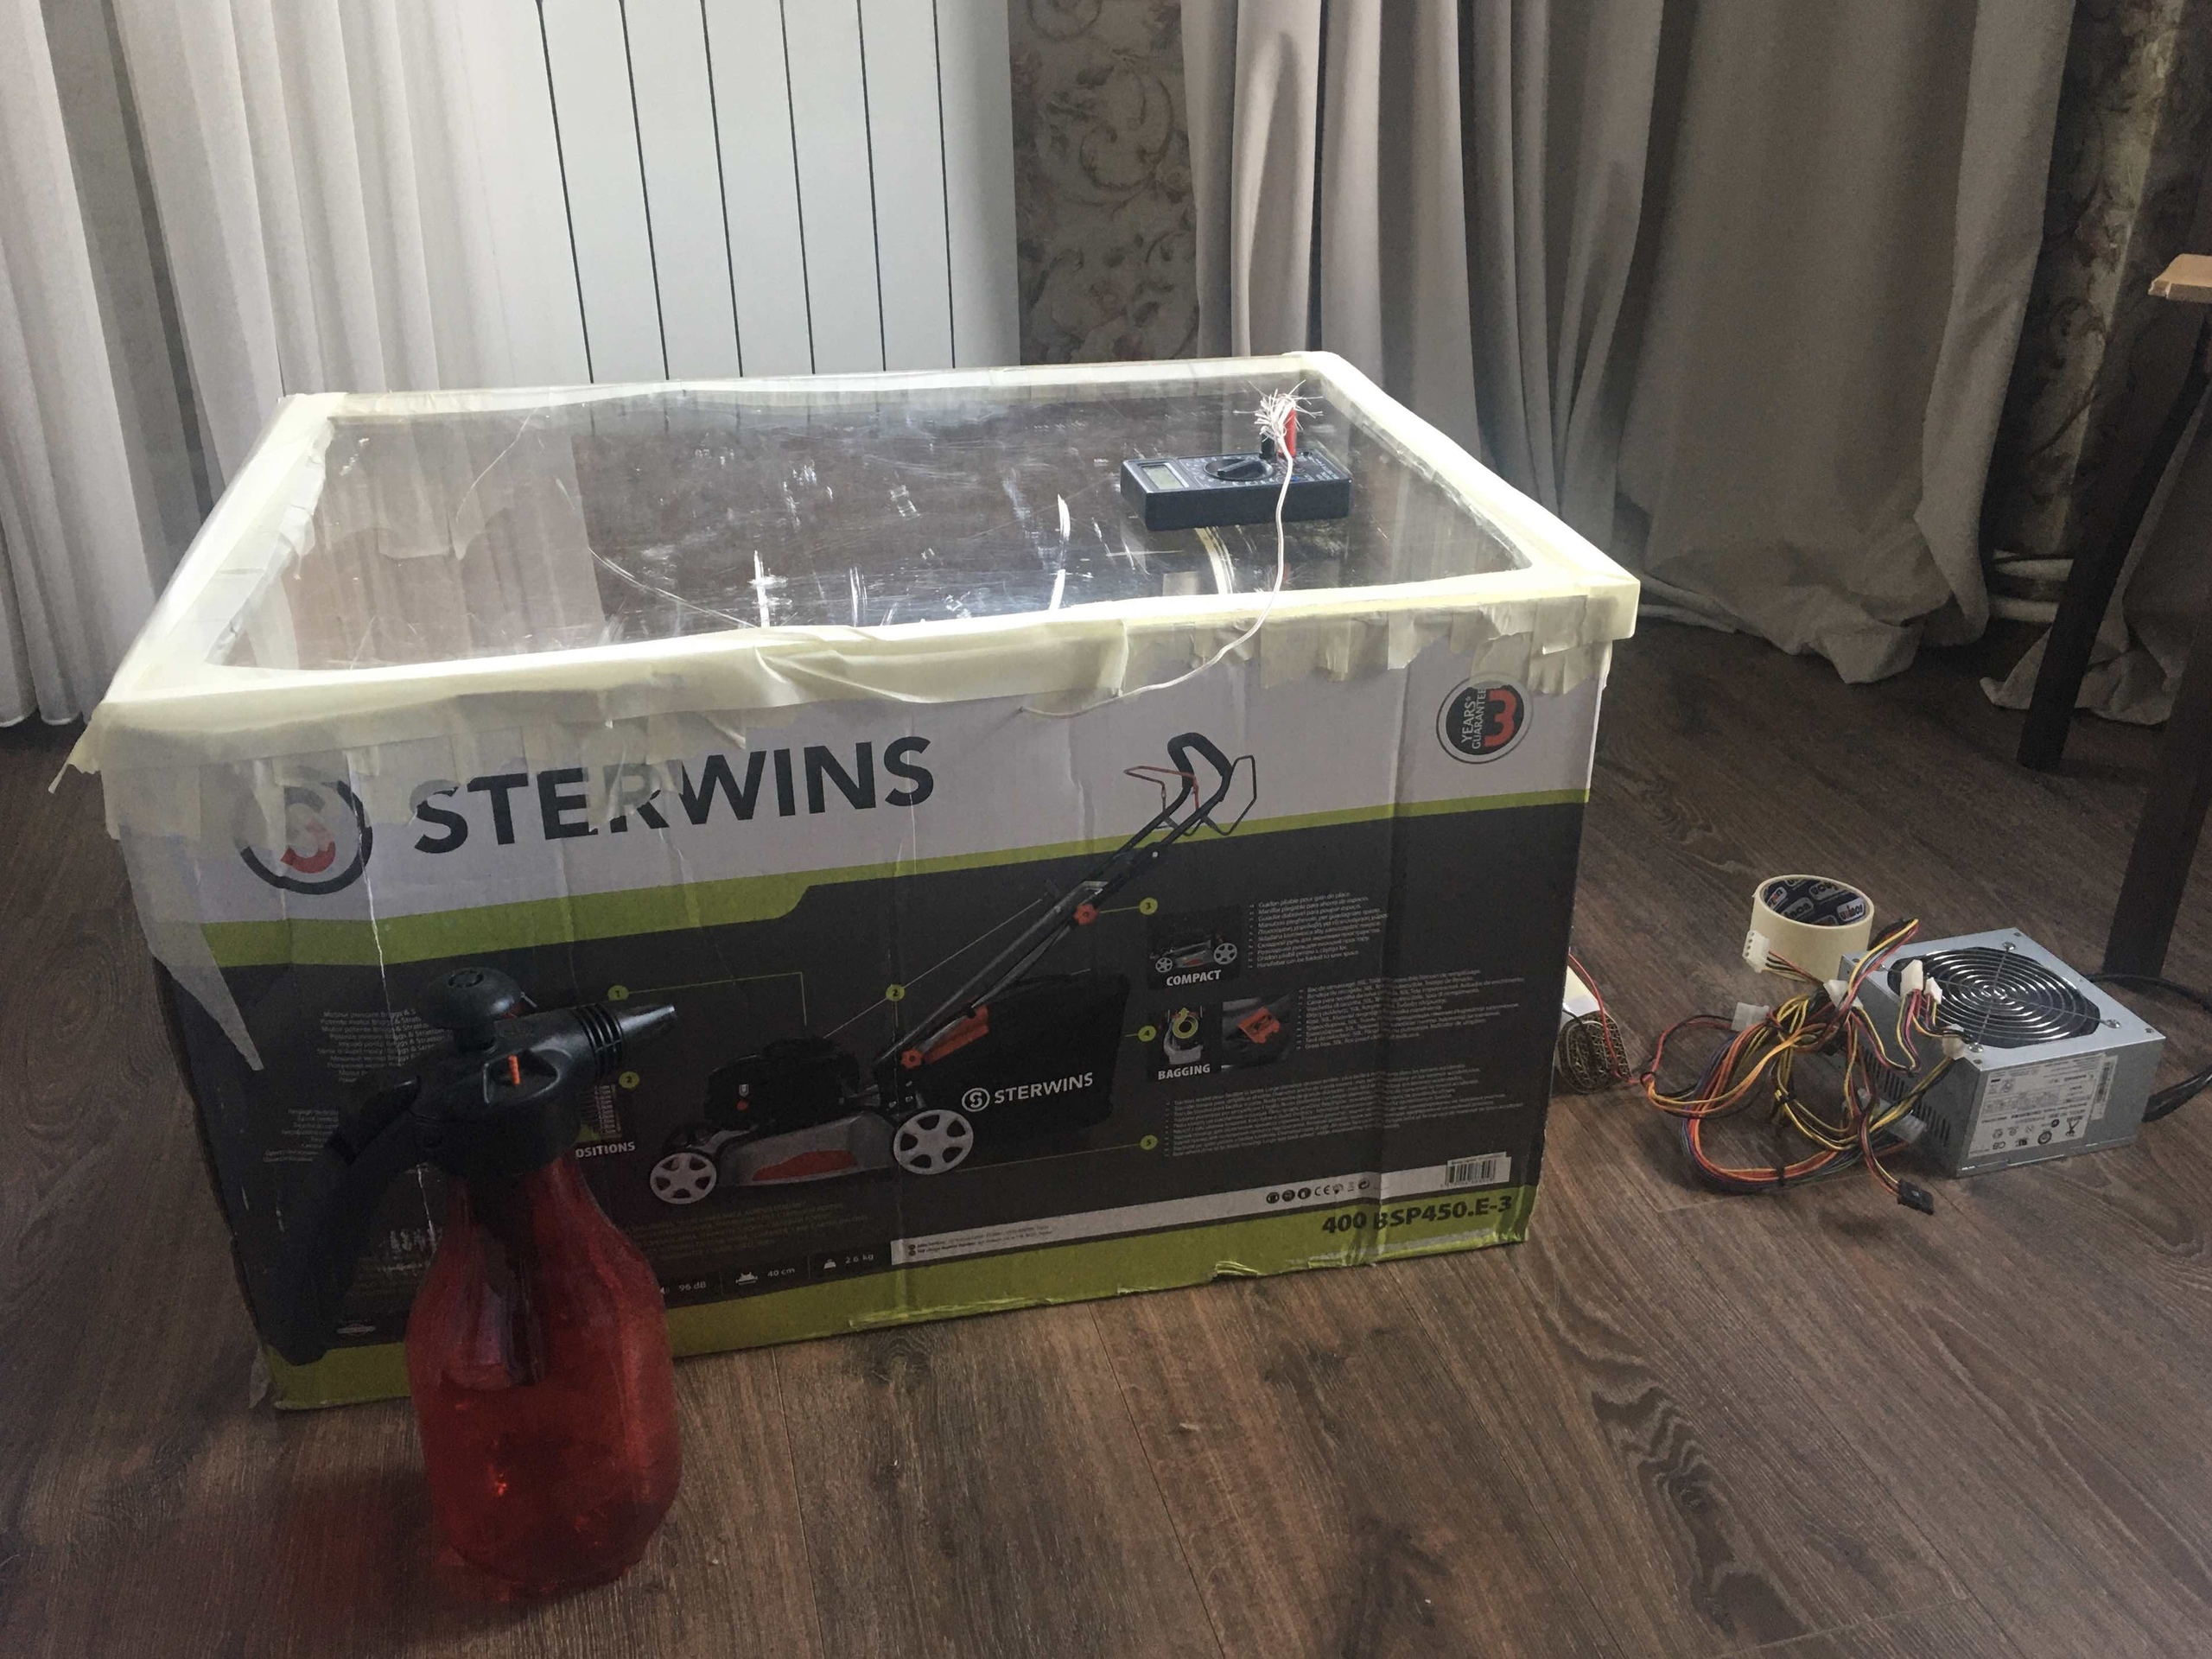
\includegraphics[width = 88mm]{pol2.jpg} \\ Подготовка к началу эксперимента}
	\end{minipage}
\end{figure}

\begin{figure}[h!]
	\centering
	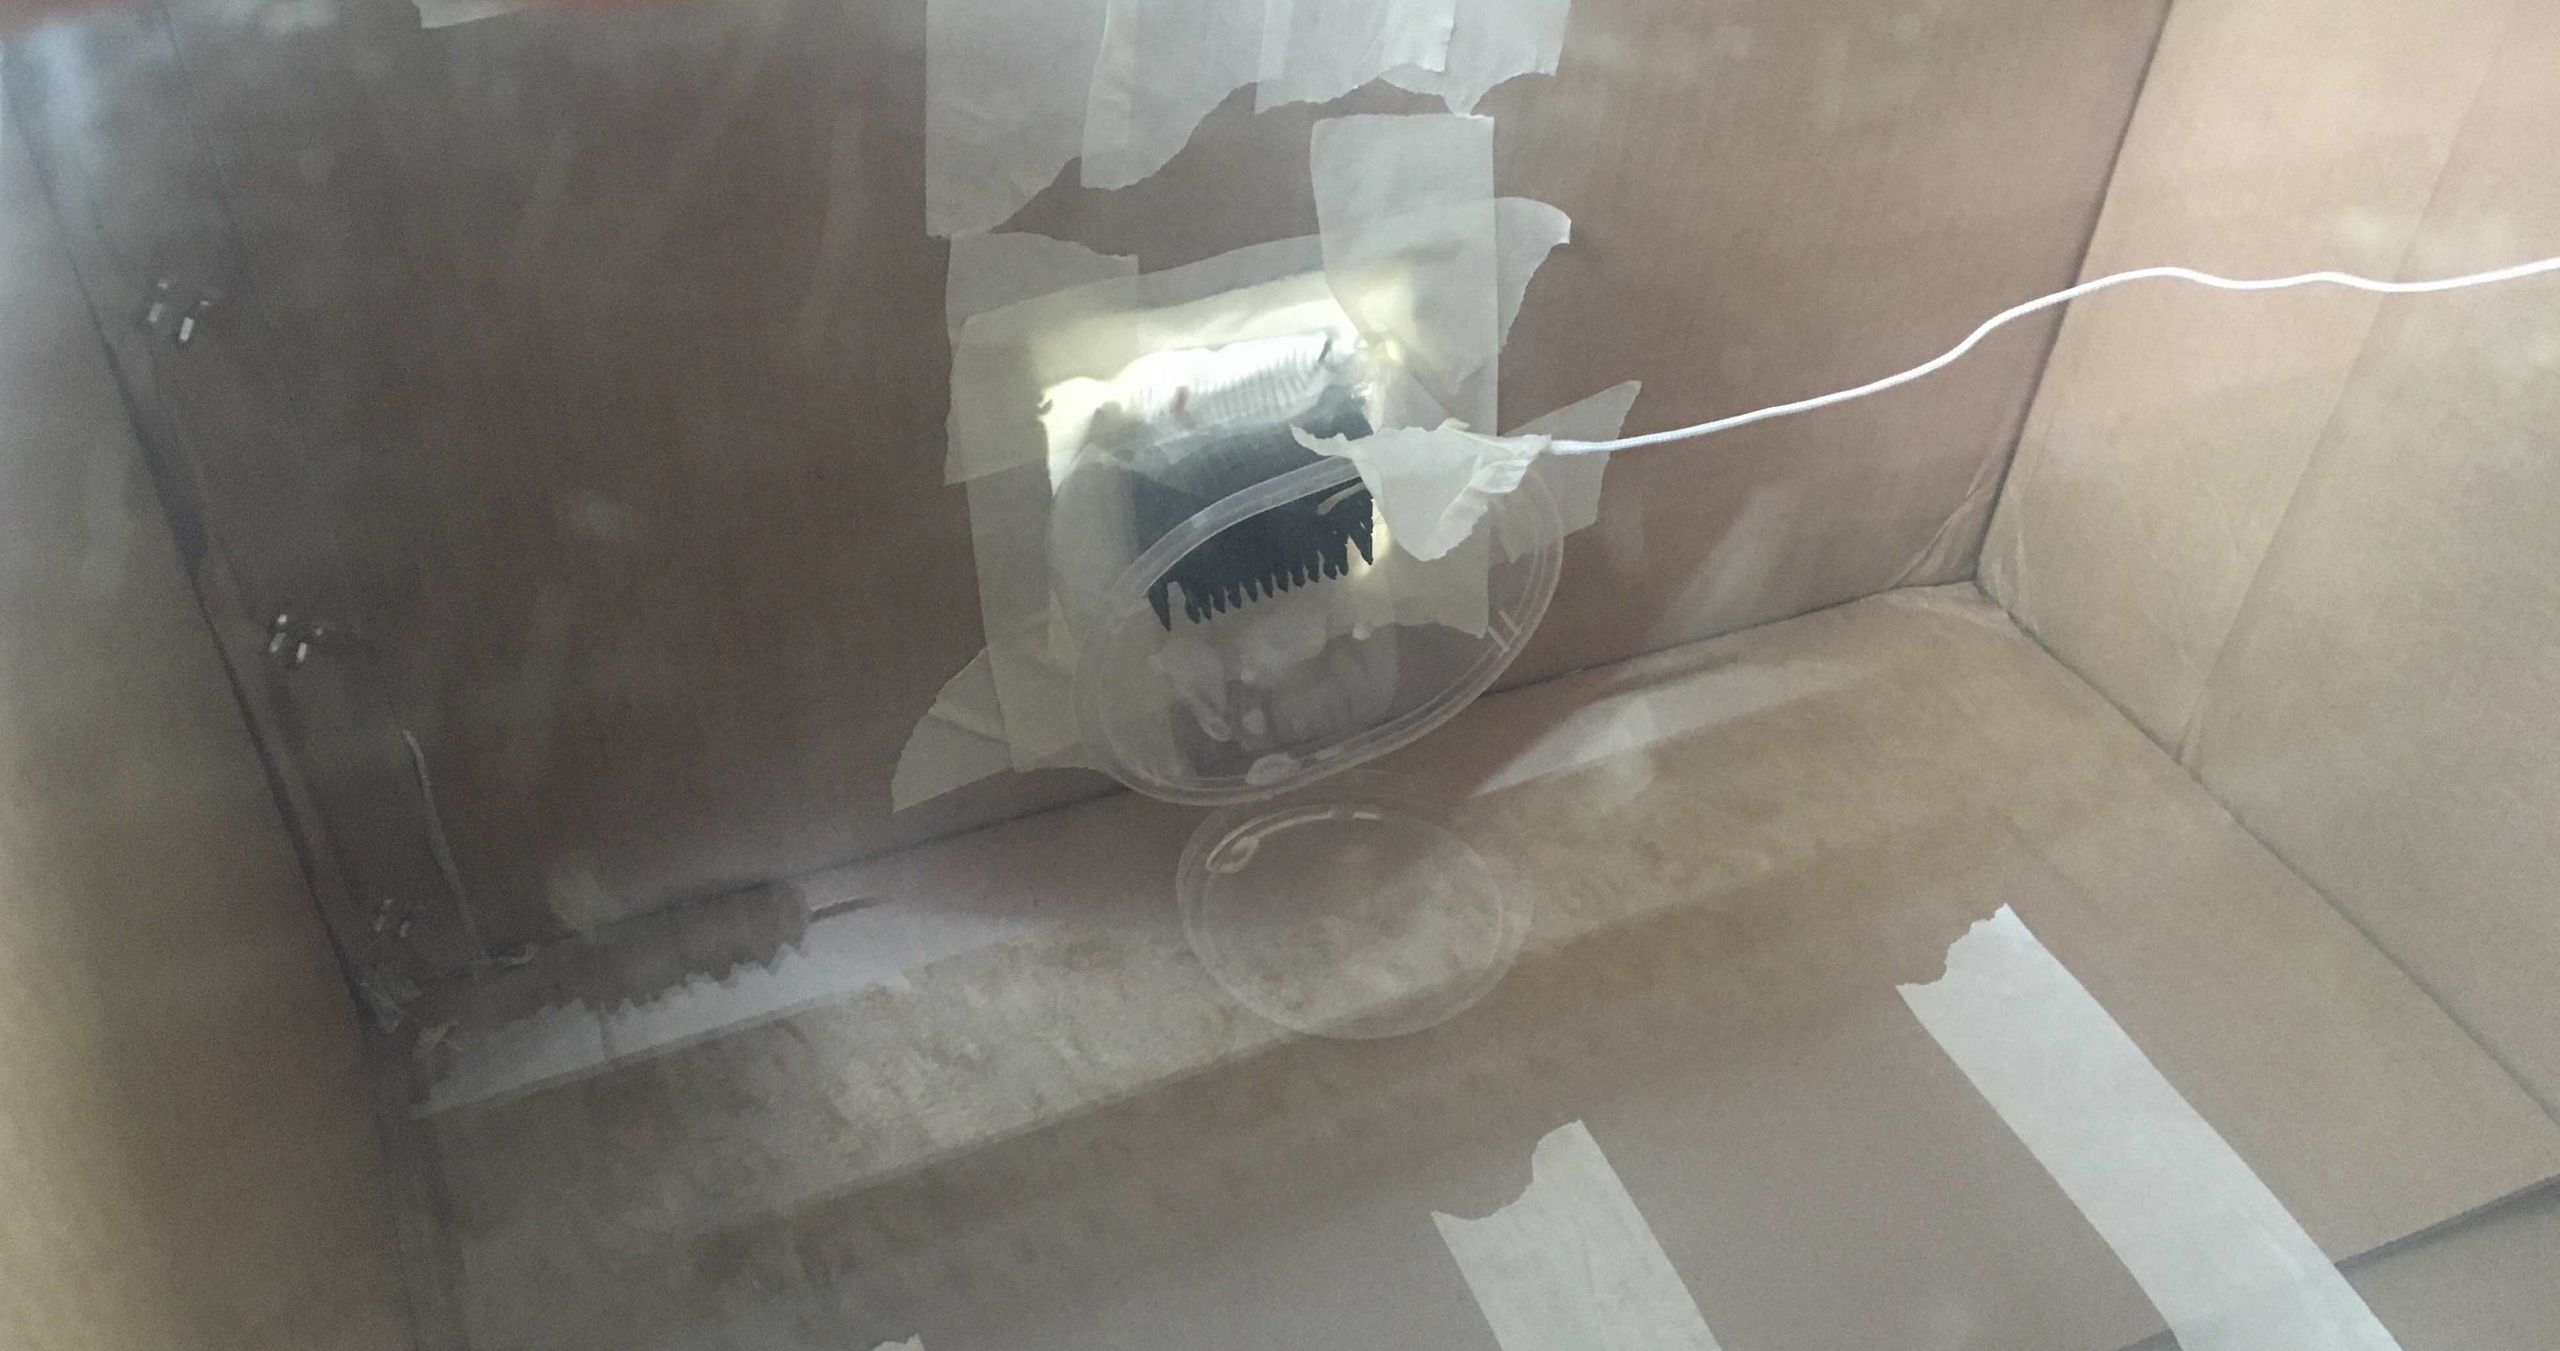
\includegraphics[scale = 0.16]{inside.jpg} \\ {\small ~Эксперимент (осушитель внутри коробки через стекло)}
\end{figure} 
\end{document}